%
% uaThesis example (for a thesis written in Portuguese)
%
% the complete list of options and commands can be found in uaThesis.sty
%

\documentclass[11pt,twoside,a4paper]{report}
%\documentclass[11pt,twoside,a4paper,openright]{report}    % Estilo relatório
% openright: página inicial de cada capítulo sempre ímpar
\usepackage[Mec,newLogo,final]{uaThesis}

\def\ThesisYear{2018}

% optional packages
\usepackage[portuguese]{babel}\addto{\captionsportuguese}{\renewcommand{\bibname}{Refer\^encias}}%Nome da Bibliografia

\usepackage{hyperref}
\usepackage{bookmark}
\usepackage{amsmath}
\usepackage{amssymb}
\usepackage{xspace}% used by \sigla

\graphicspath{ {Pictures/} }
    % Símbolos da American Mathematical Society
    \usepackage{mathtools}
    %\usepackage{amsmath}
    %\usepackage[citebordercolor={1 1 1},linkbordercolor={1 1 1}]{hyperref}
    \usepackage{graphicx} % Required for the inclusion of images
    \usepackage{subcaption}   
    \usepackage{float}
    \usepackage{listings}
    \usepackage{courier}
    %\renewcommand{\ttdefault}{pcr}
    \lstset{basicstyle=\ttfamily}
    
    \usepackage{fancyhdr}                             % Utilização de fancy headings
    
    \usepackage{enumitem}
    \usepackage{makecell}
    \usepackage{pdflscape}
    \usepackage[toc,page]{appendix}
    
    %diagranas:
    \usepackage{tikz}
    \usetikzlibrary{shapes,arrows,chains,calc,backgrounds}
    \usepackage{grafcet}
    \usepackage{fancyref}
    \usepackage{pgfplots} %grafico barra
    \usepackage{pgf-pie} %package pie
    \pgfplotsset{compat=1.8}
    
%    \usepackage[url = false, backend=biber, style = numeric, sorting=none]{biblatex}
%    \addbibresource{bib/own/molde.bib}


%encoding
%--------------------------------------
\usepackage[utf8]{inputenc}
\usepackage[T1]{fontenc}
%--------------------------------------

%-------------------------------------------------------------
% Preâmbulo do documento - Definições da tese
% -------------------------------------------------------------
\newcommand{\authorname}{Bruno Manuel de Moura Ramos}         % Nome do autor da tese
\newcommand{\thesistitle}{Sistema de Recolha e Armazenamento Remoto de Informação Sensorial de um Processo Industrial usando Bases de Dados Múltiplas} % Título da tese
\newcommand{\thesisyear}{2018}                                % Ano da tese
\newcommand{\thesisdegree}{Mestrado}                          % Grau
\newcommand{\sciarea}{Engenharia Mecânica}                    % Área científica da tese
% -------------------------------------------------------------\usepackage{forest}

% Preâmbulo do documento - Equipa de orientação
% -------------------------------------------------------------
\newcommand{\profdoc}{Prof. Doutor}                            % Grau geral
\newcommand{\supervisor}{Vitor Manuel Ferreira dos Santos}                  % Orientador
\newcommand{\supdegree}{Professor Associado}                   % Grau académico do orientador
\newcommand{\supfili}{Departamento de Engenharia Mecânica}    % Filiação do orientador
\newcommand{\cosupervisor}{Jorge Augusto Fernandes Ferreira}        % Co-orientadorScreenshot from 2017-06-06 17-44-04
\newcommand{\cosupdegree}{Professor Auxiliar}              % Grau académico do co-orientador
\newcommand{\cosupfili}{Departamento de Engenharia Mecânica}     % Filiação do co-orientador
\newcommand{\cosupuni}{Universidade de Aveiro}                 % Instituição do co-orientador
% -------------------------------------------------------------
% Preâmbulo do documento - Membros do júri
% -------------------------------------------------------------
\newcommand{\tribpresident}{José Paulo Oliveira Santos}                    % Presidente do júri
\newcommand{\tribpresidentcat}{Professor Auxiliar}         % Categoria do presidente do júri
\newcommand{\tribi}{Carlos Manuel Azevedo Costa}                  % Elemento do júri 1
\newcommand{\tribicat}{Professor Auxiliar}                   % Categoria do elemento do júri 1
\newcommand{\tribifili}{Universidade de Aveiro }              % Filiação do elemento do júri 1
\newcommand{\tribii}{Juri2}                      % Elemento do júri 2
\newcommand{\tribiicat}{Professor Auxiliar}                   % Categoria do elemento do júri 2
\newcommand{\tribiifili}{Instituto Superior de Gestão}        % Filiação do elemento do júri 2


\setlength{\parskip}{0em}
% optional (comment to use default)s
%   depth of the table of contents
%     1 ... chapther and sections
%     2 ... chapters, sections, and subsections
%     3 ... chapters, sections, subsections, and subsubsections
\setcounter{tocdepth}{3}

% optional (comment to used default)
%   horizontal line to separate floats (figures and tables) from text
\def\topfigrule{\kern 7.8pt \hrule width\textwidth\kern -8.2pt\relax}
\def\dblfigrule{\kern 7.8pt \hrule width\textwidth\kern -8.2pt\relax}
\def\botfigrule{\kern -7.8pt \hrule width\textwidth\kern 8.2pt\relax}

% custom macros (could also be defined using \newcommand)
\def\I{\mathtt{i}}         % one possible way to represent $\sqrt{-1}$
\def\Exp#1{e^{2\pi\I #1}}  % argument inside braces, i.e., "{}"
\def\EXP#1.{e^{2\pi\I #1}} % argument finishes when a full stop is encountered, i.e., "."
\def\sigla{\LaTeX\xspace}  % use as "blabla \sigla blabla (no need to do "blabla \sigla\ blabla"

\def\AddVMargin#1{\setbox0=\hbox{#1}%
                  \dimen0=\ht0\advance\dimen0 by 2pt\ht0=\dimen0%
                  \dimen0=\dp0\advance\dimen0 by 2pt\dp0=\dimen0%
                  \box0}   % add extra vertical space above and below the argument (#1)
\def\Header#1#2{\setbox1=\hbox{#1}\setbox2=\hbox{#2}%
           \ifdim\wd1>\wd2\dimen0=\wd1\else\dimen0=\wd2\fi%
           \AddVMargin{\parbox{\dimen0}{\centering #1\\#2}}} % put #1 on top #2


\begin{document}

%
% Cover page (use only one of the first two \TitlePage)
%

% First alternative, with a figure
\TitlePage
  %\GRID  % for debugging ONLY
  \HEADER{\BAR\FIG{
\includegraphics[height=60mm]{uaLogoOld}}} % the \FIG{} is optional
         {\ThesisYear}
  \TITLE{\authorname}
        {Sistema de Recolha e Armazenamento Remoto de Informação Sensorial de um Processo Industrial usando Bases de Dados Múltiplas}
\EndTitlePage
\titlepage\ \endtitlepage % empty page


% Definição da capa interior
% -------------------------------------------------------------
\TitlePage
%   \PGRID                                       % Desenha grelha rectangular de 3mm
\HEADER{}{\thesisyear}
\TITLE{\authorname}
{\thesistitle}
\vspace*{15mm}
\TEXT{}
{Projeto apresentado à Universidade de Aveiro para cumprimento dos requisitos necessários à obtenção do grau de \thesisdegree{} em \sciarea, realizada sob orientação científica de \supervisor, \supdegree{} do \supfili{} da Universidade de Aveiro e de \cosupervisor, \cosupdegree{} do \cosupfili{} da \cosupuni.}
\EndTitlePage
\titlepage\ \endtitlepage                        % Página de verso em branco


% -------------------------------------------------------------
% Definição da página do júri da dissertação (PT/EN)
% -------------------------------------------------------------
\TitlePage
\vspace*{55mm}
\TEXT{\textbf{O júri~/~The jury\newline}}
{}
\TEXT{Presidente~/~President}
{\textbf{\profdoc{} \tribpresident}\newline {\small
		\tribpresidentcat{} da Universidade de Aveiro}}
\vspace*{5mm}
\TEXT{Vogais~/~Committee}
{\textbf{\profdoc{} \supervisor}\newline {\small
		\supdegree{} da Universidade de Aveiro (orientador)}}
%\vspace*{5mm}
%\TEXT{}
%{\textbf{\profdoc{} \cosupervisor}\newline {\small
%		\cosupdegree{} da \cosupfili{} (co-orientador)}}
\vspace*{5mm}
\TEXT{}
{\textbf{\profdoc{} \tribi}\newline {\small
		\tribicat{} da \tribifili (arguente principal)}}
%\vspace*{5mm}
%\TEXT{}
%{\textbf{\profdoc{} \tribii}\newline {\small
%		\tribiicat{} da \tribiifili}}
\EndTitlePage

\titlepage\ \endtitlepage                        % Página de verso em branco

\TitlePage
  \vspace*{55mm}
  \TEXT{\textbf{agradecimentos~/\newline acknowledgements}}
       {Em primeiro lugar, um agradecimento aos professores Vítor Santos e Jorge Ferreira que, sem a sua orientação e sugestões chave, não teria sido capaz de desenvolver o projeto até este ponto.\\
        \\
       Obrigado aos que participaram no desenvolvimento deste projeto, cujas sugestões e experiência ficaram gravadas na solução desenvolvida e, se for bem sucedida, seguirá para o mundo industrial.\\
        \\
       Um obrigado aos colegas do Laboratório de Automação e Robótica pela companhia e ajuda sempre que precisei.\\
        \\
       Um obrigado muito especial para os meus colegas e amigos de curso por me terem ajudado ao longo destes anos a chegar tão longe.
        \\
       Obrigado também aos que me apoiaram quando apaguei a tese sem querer e perdi o documento escrito e me convenceram que passar 5 noites sem dormir a reescrever tudo era melhor do que ir trabalhar para o \textit{McDonald's}.\\
        \\
       Por último, um muito obrigado aos meus pais. Por me aturarem todos estes anos e incentivarem-me constantemente a ser melhor.\\
        \\
       A todos, muito obrigado!}
  \TEXT{}
       {}
\EndTitlePage
\titlepage\ \endtitlepage % empty page

\TitlePage
  \vspace*{55mm}
  \TEXT{\textbf{Palavras-chave}}
       {Base de dados relacional; rede de bases de dados; múltiplas bases de dados; monitorização remota.}
  \TEXT{Resumo}
       {Os moldes de injeção são uma ferramenta essencial no mundo industrial. A fim de melhorar a qualidade do produto final e reduzir falhas, surgiu a necessidade de instrumentar e monitorizar moldes remotamente. Este projeto foca-se na parte da monitorização remota.\\
       Desenvolveu-se uma rede com múltiplas bases de dados relacionais e uma aplicação de gestão do sistema em ambiente \textit{Web}. A primeira garante uma transferência remota de valores segura e permanente de forma a criar um histórico de registos, juntamente com um gestor de \textit{backups} para organizar e proteger estes históricos. A segunda permite ao utilizador interagir com as bases de dados desenvolvidas podendo edita-las e consulta-las de forma a gerar relatórios.\\
       No desenvolvimento deste projeto utilizou-se \textit{MySQL} e a linguagem \textit{C} para criar e definir a rede de bases de dados, resultando numa solução simples e funcional a baixo nível. Utilizou-se um servidor \textit{Apache} e as linguagens \textit{PHP}, \textit{JS} e \textit{HTML} para desenvolver e implementar a aplicação de forma a que esta seja multiplataforma e garanta um acesso remoto ao utilizador.\\
       A solução proposta cumpre todos os objetivos definidos podendo ser já utilizada numa fase experimental. Existe ainda margem para desenvolvimentos futuros como melhoramentos de desempenho e novas aplicações que podem complementar a solução proposta.}
\EndTitlePage
\titlepage\ \endtitlepage % empty page

\TitlePage
  \vspace*{55mm}
  \TEXT{\textbf{Keywords}}
  {Relational database; database network; multiple databases; remote monitoring.}
  \TEXT{Abstract}
  {The injection molds are essential tools in the industrial world. In order to improve de quality of the final product and reduce fails, there is a need to instrument and monitor molds remotely. This project focuses on the remote monitoring part.\\
  A network with multiple relational databases and a system management application was developed in a Web environment. The first one ensures a secure and permanent remote transfer of values in order to create a history of records, together with a backup manager to organize and protect these histories. The second one allows the user to interact with the developed databases, editing and consulting them in order to generate reports.\\
  On this project's development it was used MySQL and C language to create and define the database network, resulting on a simple solution and functional on a low level. It was used an Apache server and PHP, JS and HTML languages to develop and implement the system managment aplication in order to be multiplatform and ensures a remote access to the user.\\
  The proposed solution fulfills all the objectives defined making it usable for an experimental trial. There is still room for future developments like performance improvement and new applications that can complement the proposed solution.}
\EndTitlePage
\titlepage\ \endtitlepage % empty page


%
% Tables of contents, of figures, ...
%

\pagenumbering{roman}
\tableofcontents

\cleardoublepage
\listoffigures

\cleardoublepage
\listoftables


% The chapters (usually written using the isolatin font encoding ...)

\cleardoublepage
\pagenumbering{arabic}
% ----------------------------------------------------------------
% Definicao de headers e footers
% ----------------------------------------------------------------
\pagestyle{fancy}
\renewcommand{\chaptermark}[1]{\markboth{\thechapter.#1}{}} % Capítulos em minúsculas
\fancyhf{}                                                  % Reset aos headers e footers
\fancyhead[LE,RO]{\thepage}                               % Header Left-Even (LE), Right-Odd (RO)
\fancyhead[LO]{\leftmark}                                 % Header Left-Odd (LO)
\fancyhead[RE]{\leftmark}                                 % Header Right-Even (RE)
\fancyfoot[LE]{\authorname}                               % Footer Left-Even (LE)
\fancyfoot[LO]{\authorname}                               % Footer Left-Odd (LO)
\fancyfoot[RE]{\textit{Projeto de \thesisdegree}}     % Footer Right-Even (RE)
\fancyfoot[RO]{\textit{Projeto de \thesisdegree}}     % Footer Right-Odd (RO)
\renewcommand{\headrulewidth}{0.25pt}                     % Espessura da linha de header
\renewcommand{\footrulewidth}{0.25pt}                     % Espessura da linha de footer
\addtolength{\headheight}{0.5pt}                          % Espaçamento para a linha

\chapter{Introdução}
\label{chap:intro}
\vspace{-0.5cm}
Para satisfazer as necessidades de uma população cada vez maior, surge a necessidade de produzir artigos em grande escala. Uma das tecnologias que se salientou neste campo, especialmente na produção com plástico, é a moldação por injeção.\par
Os fabricantes de moldes de injeção procuram formas de melhorar as suas ferramentas, como a qualidade do processo de fabrico e a qualidade dos materiais usados na sua construção. No entanto, dada a complexidade do processo e a quantidade de variáveis envolvidas surge a necessidade de instrumentar e monitorizar o molde de forma a garantir um controlo de qualidade. Num esforço conjunto com outros projetos e dissertações
% do Departamento de Engenharia Mecânica da Universidade de Aveiro 
procura-se dar mais um passo na monitorização dos moldes de injeção.\par
O comportamento destas ferramentas pode não se alterar de forma imediata mas alterar-se lentamente ao longo do seu tempo de vida. Para analisar esta alteração do comportamento procura-se uma forma de garantir a criação de um histórico da resposta térmica e integridade estrutural em pontos críticos de um molde de injeção. Dado que os moldes são produzidos para vários clientes pode tornar-se difícil coordenar os históricos desenvolvidos. Este projeto descreve uma solução capaz de coordenar e armazenar tais históricos mantendo a informação organizada e disponível a qualquer momento.\par 
Propõe-se armazenar a informação gerada localmente nos clientes num sistema central situado na empresa que fabrica os moldes. Esta ligação entre os sistemas locais e central, representada na \autoref{fig:intro1}, visa ser segura, atempada e sem interferência nos processos produtivos. Quanto ao método de armazenamento, propõem-se usar bases de dados relacionais que satisfaçam os requisitos propostos no projeto.\par
Para consultar a informação nas bases de dados propõem-se uma aplicação de gestão do sistema em ambiente \textit{Web}, disponível em qualquer momento, lugar e dispositivo. Esta aplicação deve permitir que utilizadores sem conhecimentos sobre bases de dados comuniquem com elas de forma a consultar a informação desejada. Assim sendo, enumeram-se os objetivos principais do projeto:
\begin{enumerate}
	\item Criar uma infraestrutura de bases de dados adequada à recolha e armazenamento em tempo real de dados sensoriais
	\item Criar uma aplicação de gestão do sistema \textit{Web} para consultar os históricos
\end{enumerate}
Como requerimento definiu-se que deve ser dada prioridade à utilização de \textit{software} aberto. Além disto, dada a quantidade de opções disponíveis no mercado, definiu-se também que a solução desenvolvida deve ser simples de forma a promover a sua portabilidade para outras plataformas e linguagens.
\begin{figure}[H]
	\begin{center}
		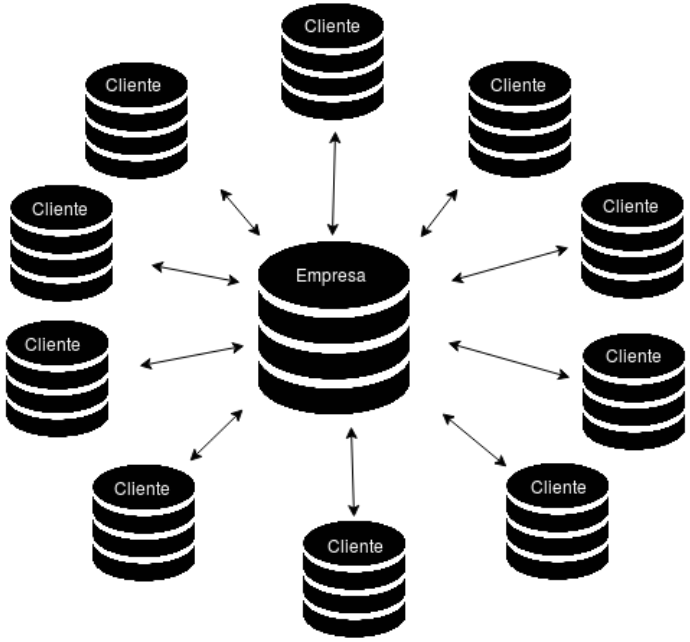
\includegraphics[width=0.6\textwidth]{Esquema_Rede} % Include the image placeholder.png
		\caption[Esquema de rede]{Esquema da rede criada com o sistema central na empresa promotora e os sistemas locais nos clientes\footnotemark}
		\label{fig:intro1}
	\end{center}
\end{figure}
\footnotetext{Ícones usados em esquemas e diagramas do projeto. URL: https://www.flaticon.com}
Este relatório está divido em 6 capítulos, distribuídos da seguinte maneira:
\begin{itemize}
	\item No \autoref{chap:intro} descreveu-se os objetivos do projeto e apresentou-se a solução proposta
	\item O \autoref{chap:conceitos} consiste na explicação de alguns conceitos necessários importantes para a criação de bases de dados relacionais e na apresentação das ferramentas utilizadas para desenvolver este projeto
	\item O \autoref{chap:solucao} explica a infraestrutura de bases de dados proposta, desenvolvida para uma utilização a baixo nível
	\item O \autoref{chap:aplicacao} descreve algumas adaptações à infraestrutura proposta e as funcionalidades da aplicação de gestão do sistema
	\item O \autoref{chap:usabilidade} apresenta resultados de testes realizados com utilizadores à aplicação de gestão do sistema
	\item O \autoref{chap:conclusoes} contém comentários sobre a solução desenvolvida e ideias para trabalhos futuros que a possam complementar
\end{itemize}

\cleardoublepage
\chapter{Conceitos e Ferramentas de Desenvolvimento}
\label{chap:conceitos}
\section{Moldes de injeção}
Moldagem é o processo mecânico de dar forma a um material no estado líquido usando um molde \cite{definicao_moldagem,definicao_moldar}. Um molde é uma ferramenta sólida oca desenvolvida para efeitos de fundição \cite{definicao_molde}. Esta é enchida com um material em estado liquido ou em pó como plástico, metal, cerâmica ou vidro \cite{Williams1975,Trovant1998,JanneyMarkA.Knoxville1991,Yan2009}.\par
A moldação por injeção é particularmente útil na produção em massa de peças de plástico com elevada complexidade geométrica \cite{Shen,Shelesh}. Estas podem ser encontradas em todas as áreas da indústria como por exemplo empacotamento, aviação, construção e eletrónica \cite{Ozcelik}. Neste processo, plástico quente é forçado para dentro de um molde frio com a forma desejada. O material ocupa todas as cavidades do molde e vai endurecendo sobre o efeito de altas pressões e arrefecimento do material. O processo de injeção pode ser divido em fases distintas \cite{Shen}:
\vspace{-0.5cm}
\begin{itemize}[noitemsep]
	\item Fecho do molde
	\item Enchimento
	\item Compactação
	\item Abertura do molde
	\item Extração
\end{itemize}
\vspace{-0.5cm}
Em 1868, John Wesley Hyatt inventou uma maneira de fazer bolas de bilhar injetando celuloide para dentro de um molde \cite{historia,patente1868}.\par
Em 1872 Jonh e o seu irmão Isaiah patentearam a primeira máquina de moldes de injeção. Esta era relativamente simples comparada às que são usadas hoje em dia na indústria. Consistia de um pequeno embolo para injetar plástico num molde através de um cilindro quente \cite{historia,patente1872}.\par
A indústria cresceu lentamente produzindo artigos de plástico como botões e pentes. Nos anos 40 a utilização de moldes de injeção cresceu devido à Segunda Guerra Mundial que tinha uma grande procura de produtos baratos e produzidos em massa \cite{historia}.\par
Em 1946, James Hendry construiu a primeira máquina de moldes de injeção com um sem fim, revolucionando a indústria dos plásticos com um design para substituir o êmbolo de Hyatt. Este sem fim é colocado dentro do cilindro e mistura o material a ser moldado antes de ser injetado no molde. Isto permitiu que cor ou plástico reciclado pudessem ser adicionados à mistura \cite{historia,patente1946}.\par
\begin{figure}[H]
	\begin{center}
		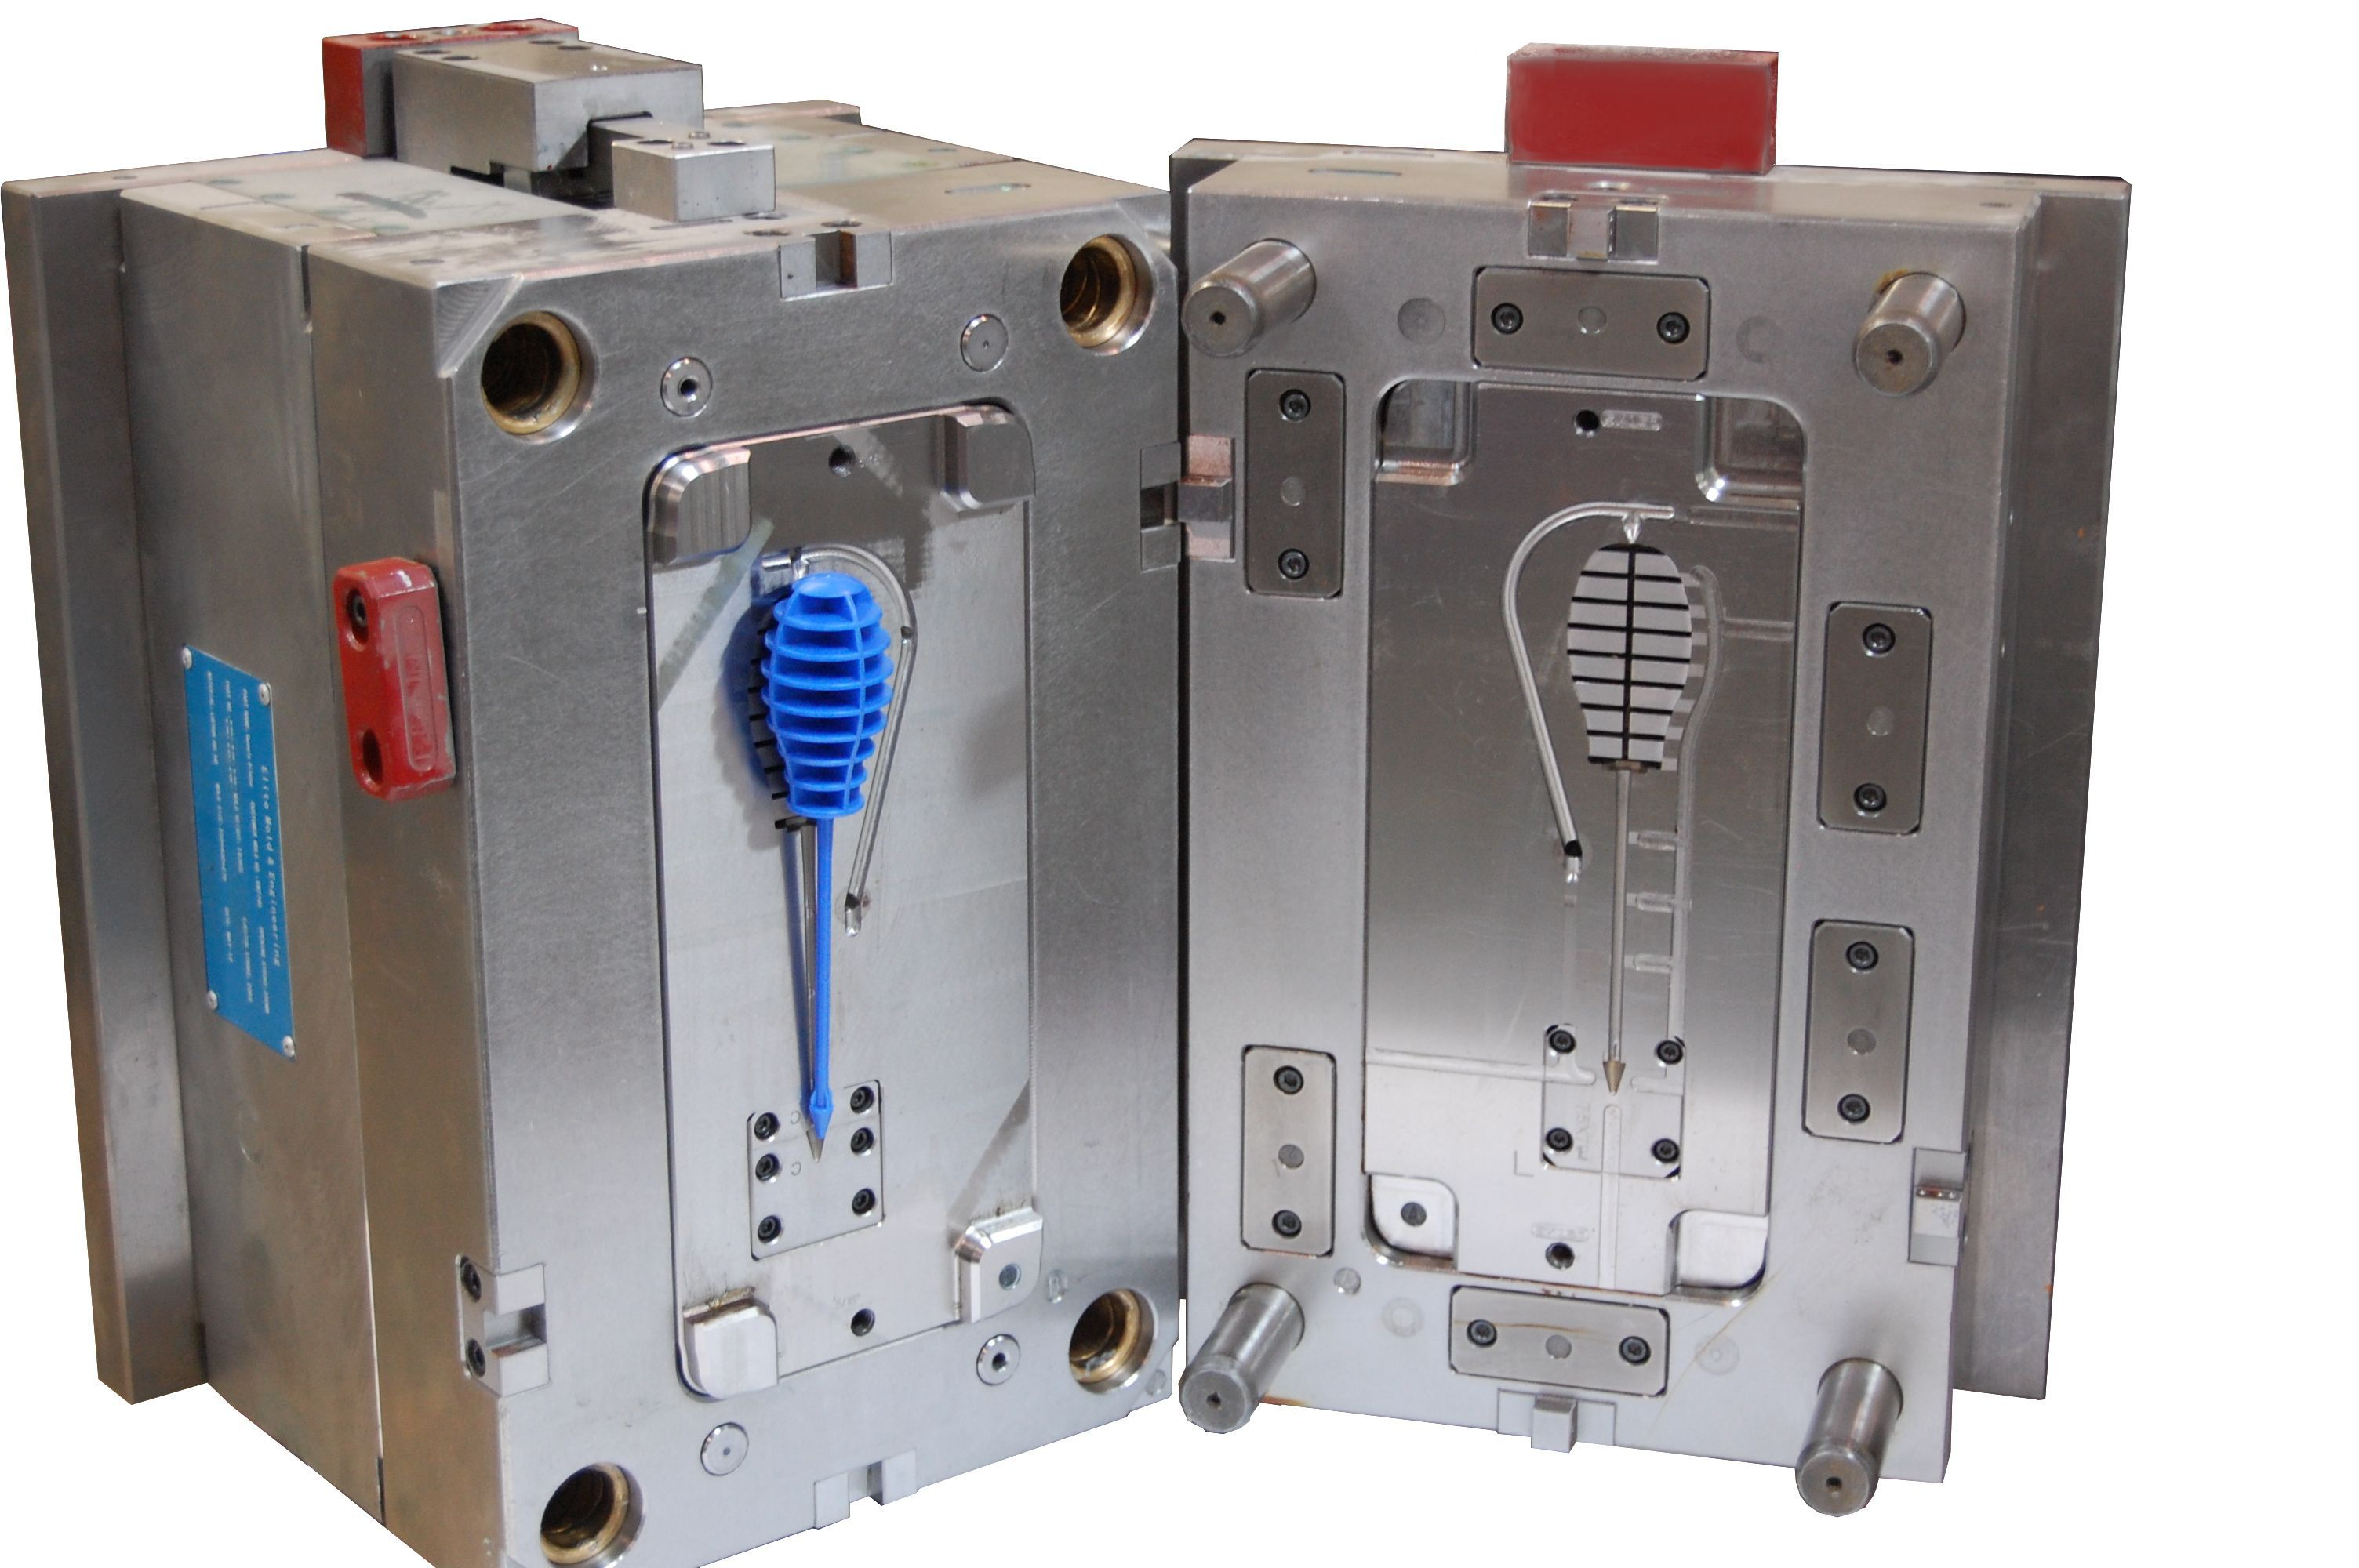
\includegraphics[width=0.70\textwidth]{molde} % Include the image placeholder.png
		\caption[Molde de injeção]{Molde de injeção aberto com a peça realizada \footnotemark}
		\label{fig:molde}
	\end{center}
\end{figure}
\footnotetext{Imagem Molde de Injeção Aberto. URL: https://i1.wp.com/www.teameliteonline.com/wp-content/uploads/2015/08/colored-part-large-mold-with-part.jpg?fit=3008\%2C2000\&ssl=1}
A qualidade de fabrico dos moldes e das peças produzidas evoluiu com o passar do tempo. A indústria investiu em técnicas sofisticadas no desenvolvimento de moldes, para que estes não contenham falhas, e no uso de materiais com qualidade elevada para evitar o desgaste da ferramenta. No entanto, dificilmente se atinge peças com a qualidade desejada unicamente através das ferramentas desenvolvidas. É necessário implementar também técnicas de monitorização de qualidade \cite{Woll}.\par 
As técnicas de monitorização e controlo de qualidade dos moldes de injeção envolvem principalmente \textit{Artificial Neural Networks} (\textit{ANNs}) e algoritmos genéricos (em inglês \textit{GA}), que analisam variáveis geradas no molde e adaptam o comportamento da ferramenta. Estes sistemas são aplicados diretamente durante a produção do molde e em circuito fechado \cite{Woll,Cook}. Neste projeto, procura-se uma solução que crie um histórico das variáveis dos moldes para determinar alterações no comportamento da ferramenta devido ao desgaste. Apesar de terem objetivos diferentes, prevê-se que, no futuro, a solução desenvolvida possa complementar, de alguma forma, as tecnologias de controlo de qualidade existentes na indústria.

\section{Base de dados relacional}
Bases de dados (BDs) e sistemas de gestão de bases de dados (SGBDs) são uma componente essencial na vida da sociedade moderna: muitos de nós realizamos ações todos os dias que envolvem interações com bases de dados. Por exemplo, o ato de depositar e levantar dinheiro num banco, reservar estadias e voos ou comprar alguma coisa \textit{online}, podem envolver alguém ou um algum programa informático que acede a uma BD \cite{Elmasri:2010:FDS:1855347}.\par
Esta tecnologia tem um impacto cada vez maior no uso dos computadores. É seguro afirmar que as BDs desempenham um papel crítico em quase todas as áreas onde são usados computadores \cite{Elmasri:2010:FDS:1855347}.\par
Uma base de dados é uma coleção organizada de dados que estão relacionados e que podem ser partilhados por múltiplas aplicações \cite{definicao_base_dados}. São considerados dados factos reais que podem ser registados e têm um significado implícito, como por exemplo, nomes, moradas e números de telefone. Uma BD tem uma fonte de onde os dados são provenientes, algum grau de interação com eventos do mundo real e uma audiência que está ativamente interessada no seu conteúdo \cite{Elmasri:2010:FDS:1855347}.\par
A implementação destas é garantida por parte de um SGBD. Este é um \textit{software} que facilita os processos de definir, construir, manipular e partilhar bases de dados entre vários utilizadores e aplicações. Definir uma BD envolve especificar o tipo de dados, as estruturas e as restrições dos dados a serem armazenados. Construir é o processo de guardar dados e armazená-los num local definido pelo SGBD. Manipular inclui funções como realizar \textit{queries} à BD e receber informação específica, alterá-la de acordo com mudanças nas variáveis e gerar relatórios a partir dos dados presentes. Partilhar permite que múltiplos utilizadores e programas acedam à BD simultaneamente \cite{Elmasri:2010:FDS:1855347}.\par
Outras funções importantes fornecidas pelos SGBDs incluem proteger e manter a base de dados durante um longo período de tempo. Proteger inclui proteção contra falhas de \textit{hardware} e \textit{software} e segurança contra acessos maliciosos ou não autorizados. Tipicamente uma grande BD pode ter um tempo de vida de vários anos, pelo que o SGBD tem de fornecer ferramentas para manter a BD de forma a permitir que o sistema evolua com novos requerimentos que surjam ao longo do tempo \cite{Elmasri:2010:FDS:1855347}.
Para completar estas definições iniciais, chamamos sistema de base de dados ao conjunto das BDs com o SGBD como representado na \autoref{fig:relacional1}.
\begin{figure}[H]
	\begin{center}
		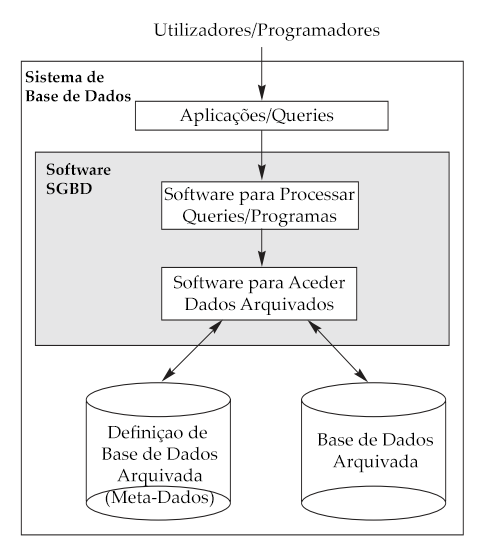
\includegraphics[width=0.6\textwidth]{SGBD} % Include the image placeholder.png
		\caption[Esquema de um sistema de bases de dados]{Esquema simplificado de um sistema de bases de dados \cite{Elmasri:2010:FDS:1855347}}
		\label{fig:relacional1}
	\end{center}
\end{figure}
O modelo relacional foi primeiramente introduzido por Ted Codd do \textit{IBM Research} em 1970 \cite{Elmasri:2010:FDS:1855347,Codd} e atraiu imediatamente atenção pela sua simplicidade e base matemática. O modelo utiliza o conceito matemático de $ " $relação$ " $ representado por tabelas e baseia-se na teoria dos conjuntos \cite{Elmasri:2010:FDS:1855347}.\par
As primeiras implementações comerciais do modelo relacional ficaram disponíveis no início dos anos 80, como o \textit{SQL/DS} no sistema operativo \textit{MVS} do \textit{IBM} e o SGBD \textit{Oracle}. Desde aí, o modelo tem sido implementado num grande número de sistemas comerciais. Os SGBDs relacionais populares atualmente incluem \textit{DB2} e \textit{Informix Dynamic Server} (do \textit{IBM}), \textit{Oracle} e \textit{Rdb} (da \textit{Oracle}), \textit{Sybase} (da \textit{Sybase}) e \textit{SQLServer} e \textit{Access} (da \textit{Microsoft}). Existem também vários sistemas gratuitos como \textit{MySQL} e \textit{PostgreSQL} \cite{Elmasri:2010:FDS:1855347}.\par
Modelos de dados que procederam o relacional, incluem os modelos hierárquicos e de rede. Estes foram propostos e implementados nos primeiros SGBDs nos anos 60 e 70. Estes modelos tiveram bastante importância na história das bases de dados e são referidos atualmente como SGBDs \textit{legacy} \cite{Elmasri:2010:FDS:1855347}.

\subsection{Domínios, Atributos, Tuplos e Relações}
Um domínio é um conjunto atómico de valores. Atómico significa que cada valor num dado domínio é único e indivisível. Um método comum de especificar um domínio é especificar o tipo de dados do mesmo. Além disto, também é útil dar nomes aos domínios. Por exemplo, a informação de números de telemóvel pode ser guardada num domínio onde o seu tipo de dados é um inteiro de nove dígitos \cite{Elmasri:2010:FDS:1855347}.\par
Um esquema de relação é constituído por um nome de uma relação e uma lista de atributos. Cada atributo é o nome do papel desempenhado por um domínio no esquema da relação. É possível múltiplos atributos terem o mesmo domínio \cite{Elmasri:2010:FDS:1855347}.\par 
O esquema de relação é um grupo de múltiplos tuplos. Cada tuplo é um conjunto de valores ordenados que estão associados diretamente a um atributo \cite{Elmasri:2010:FDS:1855347}. A \autoref{fig:relacional2} representa um exemplo do que foi dito anteriormente.
\vspace{2cm}
\begin{figure}[H]
	\hspace{-2cm}
	
		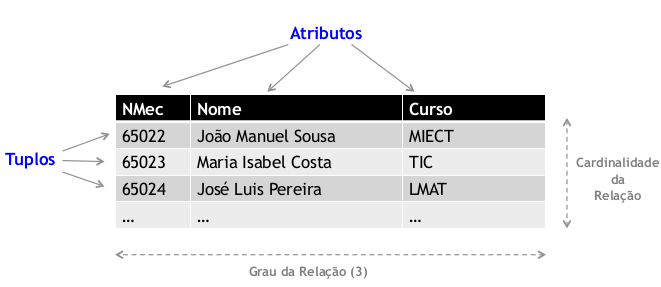
\includegraphics[width=0.9\textwidth]{exemplo_relacional} % Include the image placeholder.png
		\caption[Exemplo de atributos e tuplos]{Exemplo onde é possível observar a relação com os seus atributos e alguns tuplos}
		\label{fig:relacional2}
	
\end{figure}

\newpage
\subsection{Análise de requisitos}
A análise de requisitos é o primeiro passo necessário para definir uma base de dados. Este processo envolve uma comunicação com a entidade que deseja adquirir a BD e pode ser sumariado nos seguintes passos \cite{analise_requisitos}:
\begin{enumerate}
	\item Numa primeira fase realiza-se uma recolha detalhada de toda a informação referente ao problema do mundo real e retirar entidades, atributos, restrições, etc.
	\item Filtrar a informação de forma a remover redundâncias e informação pouco relevante
	\item Completar o problema com informação adicional necessária
	\item Distinguir dados de operações
\end{enumerate}
Este processo é transversal ao modelo de dados escolhido para construir a BD. Para uma BD relacional é necessário identificar as chaves de uma relação \cite{chaves}:
\begin{itemize}
	\item Superchave - Conjunto de atributos que identificam de forma única dois tuplos distintos
	\item Chave candidata - são todas as superchaves que não podem ser mais simplificadas
	\item Chave primária - escolhida do conjunto de chaves candidatas e identifica de forma única o tuplo
	\item Chave única - restantes chaves candidatas que não foram escolhidas como chave primária
	\item Chave estrangeira - conjunto de atributos que é chave primária de outra relação
\end{itemize}
A escolha da chave primária pode ser feita de forma aleatória mas priorizam-se chaves que identifiquem de forma natural um atributo \cite{chaves}. Por exemplo, uma pessoa pode ser identificada por um número de identificação, por um número de identificação fiscal ou pelo seu número de telefone dado que estes nunca se repetem. O número de identificação é mais natural para identificar uma pessoa do que o seu número de identificação fiscal e menos volátil do que o seu número de telefone, dado que este pode ser alterado.\par 
Para realizar um Diagrama Entidade/Relação são necessárias informações sobre a relação entre as entidades, a cardinalidade e a obrigatoriedade de participação na relação. Estas são deduzidas durante a análise de requisitos mas serão explicadas na \autoref{subchap:DER}.

\subsection{Diagrama Entidade Relação}
\label{subchap:DER}
A representação lógica dos dados é uma componente importante na área das bases de dados. Existem vários modelos para esta representação antes da criação do modelo entidade-relação apresentado por P. P. Chen em 1976, sendo os mais conhecidos os modelos em rede, relacional e entidade. Estes modelos têm as suas vantagens e desvantagens. O modelo em rede permite uma vista mais natural dos dados dividindo-os em entidades e relações (até um determinado ponto), mas a sua capacidade de garantir independência dos dados foi superada. O modelo relacional consegue ter um grande grau de independência dos dados, mas pode perder alguma informação semântica importante sobre o mundo real. O modelo de entidade também consegue um grande grau de independência dos dados, mas a forma visualizar os dados não é tão fácil para algumas pessoas \cite{analise_requisitos,Chen}.\par
O modelo entidade-relação adota uma vista mais natural em que o mundo real consiste de entidades e relações, incorpora alguma informação semântica importante sobre o mundo real e consegue ter um grande grau de independência de dados. O modelo entidade-relação é baseado na teoria das relações e foi desenvolvido com o objetivo de servir de base para um sistema de visualização de dados unificado \cite{analise_requisitos,Chen}.\par
O Diagrama Entidade/Relação (DER) é uma representação gráfica da análise de requisitos realizada anteriormente baseada no modelo entidade-relação. Este diagrama não é determinístico pois, para uma mesma análise, podem nascer diferentes diagramas que cumprem todos os requisitos.\par
Um diagrama é constituído elementos como entidades, atributos e relações. Uma entidade é algo que existe no mundo real como uma pessoa ou um carro. Um atributo é uma característica da entidade como uma pessoa tem um nome e um carro tem uma matricula. Uma relação é como uma ou mais entidades interagem entre si, como uma pessoa tem um carro \cite{analise_requisitos,Chen}.\par 
Passando à notação, as entidades são representadas por caixas retangulares, os atributos por caixas ovais e as relações por caixas em forma de losango, como mostra a \autoref{fig:der1}. Os atributos sublinhados representam a chave primária da entidade \cite{analise_requisitos,Chen}.
\begin{figure}[H]
	\begin{center}
		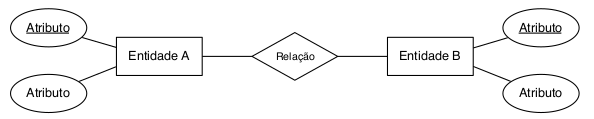
\includegraphics[width=0.8\textwidth]{notacao1} % Include the image placeholder.png
		\caption[Representação de entidades, relações e atributos]{Representação das entidades Pessoa e Carro, uma pessoa identificada pelo número de ID civil tem um carro identificado pela sua matrícula}
		\label{fig:der1}
	\end{center}
\end{figure}
As entidades podem ser fortes e fracas. Uma entidade forte não depende de outras entidades, enquanto uma entidade fraca necessita de ser identificada em conjunto com uma entidade forte. As relações de identificação definem a ou as entidades fortes que identificam uma entidade fraca entre as quais esta se relaciona. As entidades fracas são representadas por caixas retangulares com linha dupla e as relações de identificação são identificadas por um losango de linha dupla como representado na \autoref{fig:der2} \cite{analise_requisitos}.
\begin{figure}[H]
	\begin{center}
		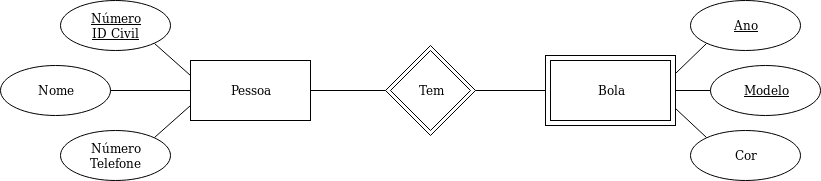
\includegraphics[width=0.8\textwidth]{notacao2} % Include the image placeholder.png
		\caption[Representação de entidades fortes e fracas e relação de identificação]{Representação das entidades Pessoa e Bola, uma pessoa identificada pelo número de ID civil tem uma bola de um determinado modelo e ano. A bola não tem um elemento caracterizador único pois podem existir bolas do mesmo modelo e ano, então identifica-se esta em conjunto com informação da pessoa que tem a bola}
		\label{fig:der2}
	\end{center}
\end{figure}
\newpage
Para completar a relação entre entidades é necessário identificar também o grau, cardinalidade e obrigatoriedade de participação de uma relação. Quanto ao grau, uma relação pode ser unária, binária ou ternária como representado na \autoref{fig:der3}. As relações ternárias podem ser decompostas em relações binárias, como mostra a \autoref{fig:der4} \cite{analise_requisitos}.
\vspace{2cm}
\begin{figure}[H]
	\centering
	\begin{minipage}{0.5\textwidth}
		\vspace{-1cm}
		\begin{center}
			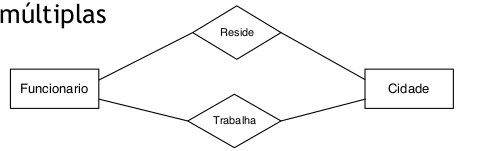
\includegraphics[width=.25\textwidth]{notacao3} % Include the image placeholder.png
			\subcaption{Exemplo de relação unária onde uma\\pessoa casa com outra pessoa}
			\label{fig:der31}
		\end{center}
	\end{minipage}%
	\begin{minipage}{0.5\textwidth}
		\begin{center}
			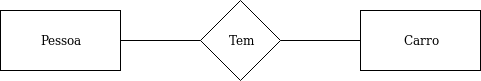
\includegraphics[width=0.9\textwidth]{notacao4} % Include the image placeholder.png
			\subcaption{Exemplo de relação binária onde uma pessoa tem um carro}
			\label{fig:der32}
		\end{center}
	\end{minipage}
	\begin{minipage}{0.5\textwidth}
		\vspace{1cm}
		\begin{center}
			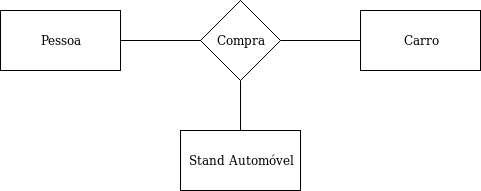
\includegraphics[width=0.9\textwidth]{notacao5} % Include the image placeholder.png
			\subcaption{Exemplo de relação ternária onde uma pessoa compra um carro a um stand automóvel}
			\label{fig:der33}
		\end{center}
	\end{minipage}
	\caption{Representação dos graus de relações}
	\label{fig:der3}
\end{figure}
\vspace{1cm}
\begin{figure}[H]
	\begin{center}
		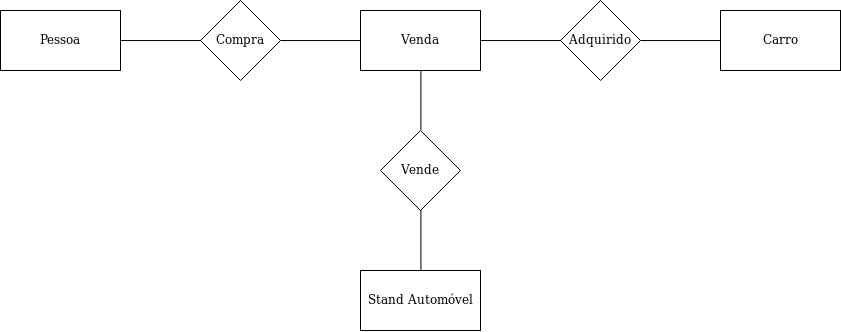
\includegraphics[width=.75\textwidth]{notacao6} % Include the image placeholder.png
		\caption[Exemplo de decomposição de uma relação ternária em relações binárias]{Exemplo de decomposição da relação ternária da \autoref{fig:der33} em relações binárias. A entidade venda relaciona de forma mais simples a pessoa, o carro e o stand automóvel envolvidos na compra}
		\label{fig:der4}
	\end{center}
\end{figure}

\newpage
As relações podem também ser múltiplas, ou seja, mais do que uma relação entre entidades como demonstrado na \autoref{fig:der8} \cite{analise_requisitos}.
\begin{figure}[H]
	\begin{center}
		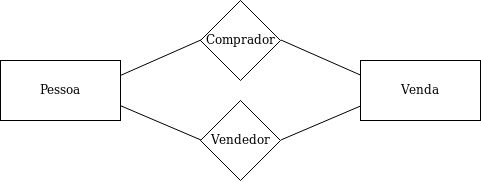
\includegraphics[width=0.5\textwidth]{notacao7} % Include the image placeholder.png
		\caption[Representação de múltiplas relações entre duas entidades]{Representação de múltiplas relações entre duas entidades, no ato de venda uma pessoa é o vendedor e outra é o comprador}
		\label{fig:der8}
	\end{center}
\end{figure}
Quanto à cardinalidade uma relação pode ser de três tipos \cite{analise_requisitos}:
\begin{itemize}[noitemsep]
	\item 1 para 1
	\item 1 para N ou N para 1
	\item N para M
\end{itemize}
A \autoref{fig:der5} apresenta uma representação visual destas cardinalidades e a \autopageref{fig:der6} apresenta a notação da cardinalidade definida por Chen \cite{analise_requisitos, Chen}.
\begin{figure}[H]
	\centering
	\begin{minipage}{0.3\textwidth}
		\vspace{-.5cm}
		\begin{center}
			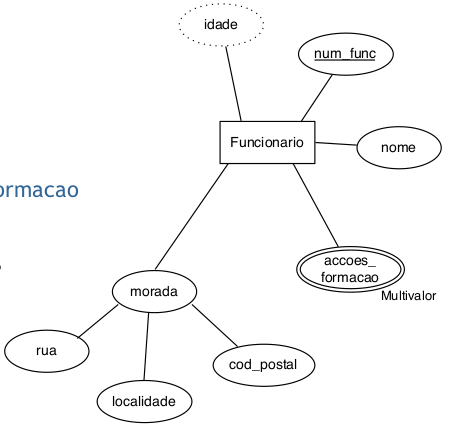
\includegraphics[width=0.4\textwidth]{notacao8} % Include the image placeholder.png
			\subcaption{Relação 1 para 1\\ou um para um}
			\label{fig:der51}
		\end{center}
	\end{minipage}%
	\begin{minipage}{0.3\textwidth}
		\begin{center}
			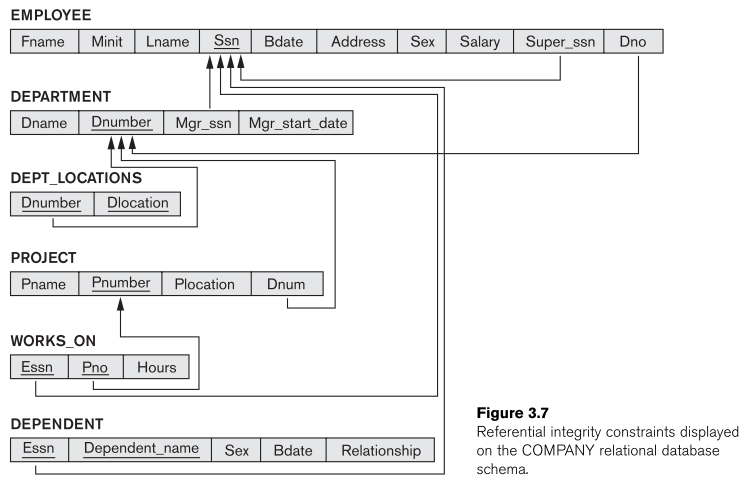
\includegraphics[width=0.4\textwidth]{notacao9} % Include the image placeholder.png
			\subcaption{Relação 1 para N\\ou N para 1\\ou um para muitos}
			\label{fig:der52}
		\end{center}
	\end{minipage}%
	\begin{minipage}{0.3\textwidth}
		\vspace{-.5cm}
		\begin{center}
			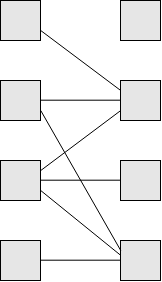
\includegraphics[width=0.4\textwidth]{notacao10} % Include the image placeholder.png
			\subcaption{Relação N para M\\ou muitos para muitos}
			\label{fig:der53}
		\end{center}
	\end{minipage}
	\caption{Representação dos tipos de cardinalidade}
	\label{fig:der5}
\end{figure}
\vspace{.5cm}
\begin{figure}[H]
	\centering
	\begin{minipage}{1\textwidth}
		\begin{center}
			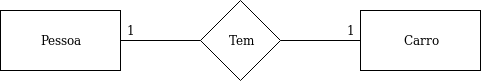
\includegraphics[width=.5\textwidth]{notacao11} % Include the image placeholder.png
			\subcaption{1 pessoa pode ter 1 carro}
			\label{fig:der61}
		\end{center}
	\end{minipage}
	\begin{minipage}{1\textwidth}
		\begin{center}
			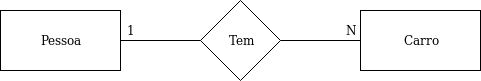
\includegraphics[width=0.5\textwidth]{notacao12} % Include the image placeholder.png
			\subcaption{1 pessoa pode ter N carros}
			\label{fig:der62}
		\end{center}
	\end{minipage}
	\caption{Notação da cardinalidade de Chen}
	\label{fig:der6}
\end{figure}
A obrigatoriedade de participação numa relação define se uma entidade tem de participar obrigatoriamente na relação. Esta é representada por uma linha dupla na ligação com a relação como representado na Figura \ref{fig:der9} \cite{analise_requisitos}. 
\begin{figure}[H]
	\begin{center}
		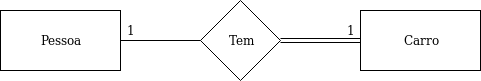
\includegraphics[width=0.5\textwidth]{notacao13} % Include the image placeholder.png
		\caption[Representação da obrigatoriedade de participação]{Representação da obrigatoriedade de participação. Neste caso uma pessoa pode ter ou não carro mas, um carro tem de pertencer sempre a uma pessoa}
		\label{fig:der9}
	\end{center}
\end{figure}
Os atributos também podem ser de tipos diferentes. Estes podem ser derivados, compostos ou multi-valor como mostra a \autoref{fig:der11} \cite{analise_requisitos}.
\begin{figure}[H]
	\begin{center}
		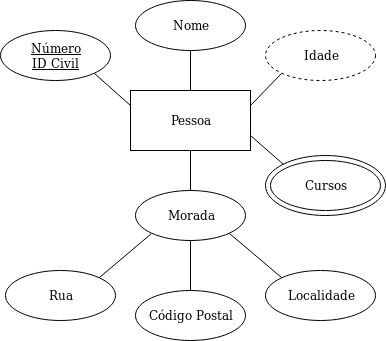
\includegraphics[width=0.5\textwidth]{notacao14} % Include the image placeholder.png
		\caption[Representação dos tipos de atributos]{Representação dos tipos de atributos. Os atributos derivados são representados a tracejado, os compostos têm sub-atributos associados a si e os multi-valor são representados com linha dupla. A idade varia com a data, uma pessoa pode ter um ou mais cursos e a morada pode ser dividida em rua, código postal e localidade}
		\label{fig:der11}
	\end{center}
\end{figure}

\subsection{Esquema Relacional}
O esquema relacional inclui todas as relações que concretizam uma base de dados. Cada relação é representada pelos seus atributos, tendo os atributos chave sublinhados. Quando um ou mais atributos de relações diferentes representam o mesmo elemento do mundo real, estes são conectados. Neste caso o conjunto de atributos é chave primária de uma relação e, nas restantes relações, estes são considerados chaves estrangeiras. São representados com uma ligação da chave estrangeira para a chave primária como demonstrado na \autoref{fig:er1} \cite{Chen}.
%Quando um elemento aparece em relações diferentes significa que numa destas, o elemento, é atributo chave da relação e assim sendo, os restantes atributos são considerados chaves estrangeiras. São representados com a ligação ao atributo que serve de chave primária como demonstrado na \autoref{fig:er1} \cite{Chen}.
\begin{figure}
	\begin{center}
		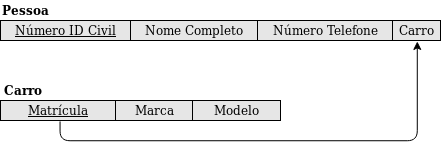
\includegraphics[width=0.7\textwidth]{notacao15} % Include the image placeholder.png
		\caption[Representação esquema relacional]{Representação do esquema relacional com as ligações das chaves estrangeiras deduzido do DER da \autoref{fig:der61}}
		\label{fig:er1}
	\end{center}
\end{figure}
Este esquema pode ser deduzido a partir do DER onde as entidades se traduzem em relações e as relações do diagrama representam as chaves estrangeiras no esquema relacional.

\section{\textit{Structured Query Language}}
\label{subchap:sql}
A linguagem \textit{Structured Query Language} (\textit{SQL}) é considerada uma das maiores razões para o sucesso comercial das bases de dados relacionais. Porque se tornou normal a sua utilização em BDs relacionais, os utilizadores tiveram menos preocupações a transferir as suas aplicações de outros tipos de BDs - por exemplo, BDs hierárquicas e em rede - para uma BD relacional. Isto porque se um SGBD não cumprisse os requisitos definidos, não era problemático transferir a solução para outro SGBD dado que ambos utilizam a mesma linguagem. Na realidade existem várias sub-versões desta linguagem dependentes de cada SGBD. No entanto, se o utilizador se limitar apenas às funções standard desta linguagem a mudança de sistema é bastante simplificada. Outra vantagem de ter uma linguagem normalizada é que uma aplicação pode utilizar informação de BDs em SGBDs diferentes ao mesmo tempo \cite{Elmasri:2010:FDS:1855347}.\par 
O nome \textit{SQL} atualmente significa \textit{Structured Query Language}. Originalmente era chamado \textit{SEQUEL} de \textit{Structured English QUEry Language}, foi desenhado e implementado no \textit{IBM Research} como uma interface experimental para o sistema de bases de dados relacionais \textit{SYSTEM R. SQL}. Um esforço conjunto entre o \textit{American National Standards Institute} (\textit{ANSI}) e a \textit{International Standards Organization} (\textit{ISO}) conduziu à normalização da versão do \textit{SQL} chamado SQL-86 ou SQL1. Surgiu depois uma versão expandida chamada SQL-92 ou SQL2. A seguinte versão reconhecida é o SQL:1999 ou SQL3. Duas atualizações depois resultaram nas versões SQL:2003 e SQL:2006  \cite{Elmasri:2010:FDS:1855347}. Sendo a atualização mais recente em 2016.\par 
O \textit{SQL} é uma linguagem básica para realizar \textit{queries} que permitem definir e construir uma BD, bem como interagir com os dados presentes nas BDs \cite{Elmasri:2010:FDS:1855347}.
%O \textit{SQL} é uma linguagem básica para realizar \textit{queries} dividida em dois campos principais, \textit{DDL} e \textit{DML}. \textit{DDL} ou \textit{Data Definition Language} são as \textit{queries} que permitem definir e construir uma base de dados. \textit{DML} ou \textit{Data Manipulation Language} são as \textit{queries} que permitem interagir com os dados\cite{Elmasri:2010:FDS:1855347}. Estas serão mais exploradas na \autoref{subchap:mysql}.

%\section{Tecnologias existentes}

\newpage
\section{\textit{Software} utilizado}
Para desenvolver as redes de bases de dados e aplicação de gestão do sistema escolheram-se os \textit{softwares} apresentados na \autoref{fig:softwares}. Como a solução será futuramente implementada em ambiente empresarial, definiu-se que não se deve usar \textit{softwares} que estejam em versão \textit{beta}. Além disto definiu-se que estes devem ser abertos.
\begin{figure}[H]
	\centering
	\begin{minipage}{0.33\textwidth}
		\vspace{.87cm}
		\begin{center}
			
\includegraphics[width=0.3\textwidth]{ubuntu} % Include the image placeholder.png
			\subcaption{\textit{Ubuntu} \footnotemark}
			\label{fig:linux}
		\end{center}
	\end{minipage}%
	\begin{minipage}{0.33\textwidth}
		\begin{center}
			
\includegraphics[width=0.4\textwidth]{gcc} % Include the image placeholder.png
			\subcaption{\textit{GNU} \footnotemark}
			\label{fig:gcc}
		\end{center}
	\end{minipage}%
	\begin{minipage}{0.33\textwidth}
		\vspace{0.9cm}
		\begin{center}
			
\includegraphics[width=0.6\textwidth]{apache} % Include the image placeholder.png
			\subcaption{\textit{Apache} \footnotemark}
			\label{fig:apache}
		\end{center}
	\end{minipage}
	\begin{minipage}{1\textwidth}
		\vspace{0.5cm}
		\begin{center}
			
\includegraphics[width=0.25\textwidth]{mysql} % Include the image placeholder.png
			\subcaption{\textit{MySQL} \footnotemark}
			\label{fig:mysql}
		\end{center}
	\end{minipage}
	\caption{Logótipos dos \textit{softwares} utilizados}
	\label{fig:softwares}
\end{figure}
\footnotetext[2]{Logo Ubuntu. URL: https://assets.ubuntu.com/v1/29985a98-ubuntu-logo32.png}
\footnotetext[3]{Logo GNU. URL: https://upload.wikimedia.org/wikipedia/commons/thumb/a/af/GNU\texttt{\char`_}Compiler\\
\texttt{\char`_}Collection\texttt{\char`_}logo.svg/2000px-GNU\texttt{\char`_}Compiler\texttt{\char`_}Collection\texttt{\char`_}logo.svg.png}
\footnotetext[4]{Logo Apache. URL: https://logodownload.org/wp-content/uploads/2018/03/apache-logo.png}
\footnotetext{Logo MySQL. URL: https://logodownload.org/wp-content/uploads/2016/10/mysql-logo.png}

\subsection{Ferramentas auxiliares}
Escolheu-se o \textit{Ubuntu} 16.04LTS como sistema operativo para os sistemas usados neste projeto, representado na \autoref{fig:linux}. Este é uma distribuição do \textit{Linux} baseado no \textit{Debian}. É um sistema operativo grátis e \textit{open source} desenvolvido pela \textit{Canonical}. A liberdade deste sistema operativo na área da programação criou uma comunidade de utilizadores que ajudam a pesquisar e desenvolver este sistema operativo \cite{ubuntu}.\par 
A \textit{Canonical} encarrega-se de garantir \textit{updates} de segurança e performance de forma regular. Apesar de não ser infalível o \textit{Linux} é um dos sistemas mais estáveis e menos provável de ser afetado por vírus, dado que a maior parte destes são desenhados para afetar sistemas operativos mais populares como o \textit{Windows} \cite{ubuntu}.\par
Escolheu-se utilizar \textit{C} no desenvolvimento deste projeto devido à afinidade com esta linguagem e com o facto do \textit{MySQL} disponibilizar protocolos oficiais de comunicação com esta linguagem e documentação apropriada \cite{mysql}.\par
O \textit{C} é uma linguagem para todos os tipos de problemas e importante no mundo da programação. Originalmente desenvolvida por Dennis Ritchie entre 1969 e 1973 no \textit{Bell Labs} e usada para re-implementar o sistema operativo \textit{Unix}. Desde então esta tornou-se uma das linguagens de programação mais popular de sempre com uma oferta de vários compiladores existentes no mercado. O \textit{C} foi então normalizado pelo \textit{ANSI} em 1989 e consequentemente pelo \textit{ISO} \cite{c}.\par 
No projeto usa-se o \textit{GNU Compiler Collection} (\textit{GCC}), representado na \autoref{fig:gcc}, como compilador dos programas em \textit{C}. Este foi desenvolvido primeiramente para o sistema operativo \textit{GNU} e focou-se em ser gratuito e garantir liberdade de programação ao utilizador. Conta com uma comunidade ativa que desenvolvem constantemente novas soluções e \textit{updates} regulares ao compilador de forma a que este não fique desatualizado \cite{gcc}.\par 
Escolheu-se utilizar \textit{Apache HTTP Server}, representado na \autoref{fig:apache} como servidor \textit{HTTP} para a aplicação \textit{Web}. Este foca-se em ser um servidor gratuito e garantir uma solução segura, eficiente e extensível \cite{apache}.\par
Lançado em 1995, tornou-se no \textit{software} mais utilizado pelas empresas para correr os seus \textit{sites}. Atualmente na versão 2.4, realizam \textit{updates} constantes ao programa para o manter estável e atualizado \cite{apache}.

\subsection{\textit{HTML}, \textit{JS} e \textit{PHP}}
Escolheu-se \textit{HTML}, \textit{JS} e \textit{PHP} para desenvolver a aplicação de gestão de sistema deste projeto. Junto com \textit{SQL} e \textit{CSS} formam o conjunto de ferramentas mais usadas no desenvolvimento de aplicações \textit{Web} no mercado, representado na \autoref{fig:web}.\par 
\textit{HTML} ou \textit{Hyper Text Markup Language} descreve a estrutura da página \textit{Web} desenvolvida. Possuí elementos que funcionam como blocos para as páginas permitindo a criação de uma interface com um utilizador. \textit{CSS} ou \textit{Cascading Style Sheets} descreve como os elementos HTML devem ser dispostos na página, permitindo o desenvolvimento de uma interface mais apelativa. \textit{JS} ou \textit{JavaScript} permite interagir e alterar o código \textit{HTML} e \textit{CSS} criando uma interface mais interativa. Permite também desenvolver códigos e funções que são executadas no browser do cliente. \textit{PHP} ou \textit{PHP:Hypertext Preprocessor} permite desenvolver funções para aplicação que executam do lado do servidor. \textit{JS} e \textit{PHP} realizam ambos funções diferindo apenas no local onde são executadas \cite{web}.\par
\begin{figure}[H]
	\begin{center}
		
\includegraphics[trim={0 3cm 0 0},clip,width=0.35\textwidth]{web} % Include the image placeholder.png
		\caption[Representação das ferramentas mais usadas para desenvolver aplicações \textit{Web}]{Representação das ferramentas mais usadas para desenvolver aplicações em ambiente \textit{Web} \footnotemark}
		\label{fig:web}
	\end{center}
\end{figure}
\footnotetext{Imagem Web Development. URL: https://www.vectorstock.com/royalty-free-vector/web-development-php-html-arrows-vector-1713552}
Sem contar com a interação com o \textit{HTML} e \textit{CSS}, o \textit{PHP} pode substituir o \textit{JS} como linguagem para criação de funções do sistema. No entanto, isto pode causar problemas de desempenho dado que o servidor terá de correr funções de todos os utilizadores. Assim sendo define-se que o uso do \textit{PHP} deve ser limitado a funções de sistema mais importantes, como conectar a uma base de dados em \textit{SQL}, e o \textit{JS} deve ser usado no desenvolvimento de funções da aplicação mais triviais.

\subsection{\textit{MySQL}}
\label{subchap:mysql}
Escolheu-se o \textit{MySQL}, representado na \autoref{fig:mysql}, como SGBD relacional para construir e utilizar as BDs relacionais usadas neste projeto, dada a sua simplicidade e velocidade de resposta. Existem outras ofertas gratuitas como o \textit{SQLite} e o \textit{PostgreSQL}. O \textit{SQLite} funciona apenas localmente e não permite uma conexão remota que se procura como solução para o problema. O \textit{PostgreSQL} é um sistema robusto que permite realizar tarefas que o \textit{MySQL} não consegue realizar. No entanto, dada a simplicidade da BD prevista nesta fase do projeto, não é necessário usar uma ferramenta tão completa e robusta \cite{mysqlvs}.\par 
O \textit{MySQL} é o mais popular e o SGBD relacional mais usado \cite{mysqlvs}. Garante um acesso múltiplo, rápido e robusto a uma BD no servidor. Foi desenvolvido para lidar com grandes quantidades de informação e \textit{softwares} com utilização massiva \cite{mysql}.\par 
O \textit{MySQL} oferece soluções gratuitas e pagas, \textit{Community} e \textit{Enterprise}, respetivamente. A primeira recebe menos atualizações e correções que a solução paga. Tem também algumas funcionalidades bloqueadas e um limite na capacidade de sensivelmente 4Gb \cite{mysql}. Estas limitações não afetam o projeto e como tal opta-se pela solução gratuita deste \textit{software}.\par
Como referido na \autoref{subchap:sql}, os vários SGBDs possuem as suas próprias sub-versões da linguagem \textit{SQL} e, o \textit{MySQL}, não é exceção. Segue-se a lista com os comandos principais utilizados neste projeto \cite{mysql}:
\begin{itemize}
	\item \textbf{SHOW DATABASES/TABLES} - mostra todas as BDs ou tabelas de uma BD (\textit{MySQL})
	\item \textbf{CREATE USER/DATABASE/TABLE} - criar utilizadores, BDs ou tabelas
	\item \textbf{DROP USER/DATABASE/TABLE} - eliminar utilizadores, BDs ou tabelas
	\item \textbf{SELECT FROM} - visualizar tuplos de uma tabela
	\item \textbf{INSERT} - inserir tuplos numa tabela
	\begin{itemize}
		\item \textbf{INTO} - se forem inseridos múltiplos tuplos e um não respeitar as restrições de integridade definidas, nenhum tuplo é inserido
		\item \textbf{IGNORE} - se forem inseridos múltiplos tuplos e um não respeitar as restrições de integridade, esse é descartado e os restantes são inseridos na tabela (\textit{MySQL})
	\end{itemize}
	\item \textbf{DELETE} - elimina tuplos de uma tabela
	\item \textbf{UPDATE} - altera tuplos de uma tabela
	\item \textbf{GRANT} - dá privilégios a um utilizador
\end{itemize}
A \textit{query} do tipo SELECT permite adicionar condições do tipo \cite{mysql}:
\begin{itemize}
	\item \textbf{WHERE} - definir parâmetros de busca de um atributo
	\item \textbf{GROUP BY} - permite agrupar informação permitindo operações matemáticas sobre valores, por exemplo: contagem, soma, média, etc.
	\item \textbf{ORDER BY} - escolher a ordem dos tuplos
\end{itemize}
As \textit{queries} do tipo DELETE e UPDATE  também permitem utilizar a condição WHERE.\par 
Na criação das tabelas atribuem-se o nome dos atributos e o seu respetivo domínio. O \textit{MySQL} oferece vários tipos de dados, dos quais foram usados \cite{mysql}:
\begin{itemize}
	\item \textbf{VARCHAR(n)} - \textit{string} com tamanho máximo n
	\item \textbf{INT} - inteiro entre -2147483648 e +2147483647
	\item \textbf{TINYINT} - inteiro entre -128 e +127
	\item \textbf{FLOAT} - numérico com casa decimais
	\item \textbf{DATETIME} - data e hora no formato AAAA-MM-DD HH:MM:SS
\end{itemize}
Define-se também as restrições de integridade \cite{mysql}:
\begin{itemize}
	\item \textbf{PRIMARY KEY} - define chave primária
	\item \textbf{UNIQUE} - define chave única
	\item \textbf{FOREIGN KEY REFERENCES} - define a chave estrangeira e o atributo de referência
	\item \textbf{CHECK} - define restrições para os atributos
\end{itemize}
Estas restrições ou \textbf{CONSTRAINTS} podem e devem ser atribuídas um nome de forma a identifica-las em mensagens de erro. Além disto é possível definir o comportamento de uma restrição de chaves estrangeiras. Quando o atributo de referencia é alterado (\textbf{ON UPDATE}) ou eliminado (\textbf{ON DELETE}) \cite{mysql}:
\begin{itemize}
	\item \textbf{NO ACTION} - não deixa realizar a ação
	\item \textbf{CASCADE} - todas as chaves estrangeiras dependentes do atributo de referencia são alteradas ou eliminadas de acordo com este
	\item \textbf{SET NULL} - altera o valor da chave estrangeira para NULL
	\item \textbf{SET DEFAULT} - altera o valor da chave estrangeira para um valor predefinido
\end{itemize}
O valor NULL representa um valor de um atributo que não existe ou é desconhecido, adiciona-se \textbf{NOT NULL} a um atributo quando este não pode ser nulo \cite{mysql}.\par 
Estes são os comandos e conceitos principais que surgem ao longo deste documento. Como referido na \autoref{subchap:sql}, e se observa aqui, o \textit{SQL} é uma linguagem simples e auto-explicativa.

\cleardoublepage
\chapter{Proposta de Solução}
\label{chap:solucao}
A infraestrutura de dados desenvolvida tem como objetivo ser simples, funcional a baixo nível e sem impor restrições na instrumentação dos moldes. Este capítulo descreve o processo de desenvolvimento das bases de dados relacionais, o método de transferência de registos, a gestão de \textit{backups}, as permissões dos utilizadores e um simples simulador de registos. No \autoref{apen:queries} encontram-se as \textit{queries} desenvolvidas para construir a solução proposta, com base na informação deste capítulo.

\section{Infraestrutura de Dados}
A instrumentação dos moldes geram registos localmente nos clientes e estes devem ser guardados numa base de dados central. Realiza-se a transferência usando protocolos TCP/IP. A fim de minimizar a perda de registos em caso de falha de conexão, coloca-se uma base de dados local em cada cliente, como representado na \autoref{fig:infra1}.
\begin{figure}[H]
	\begin{center}
		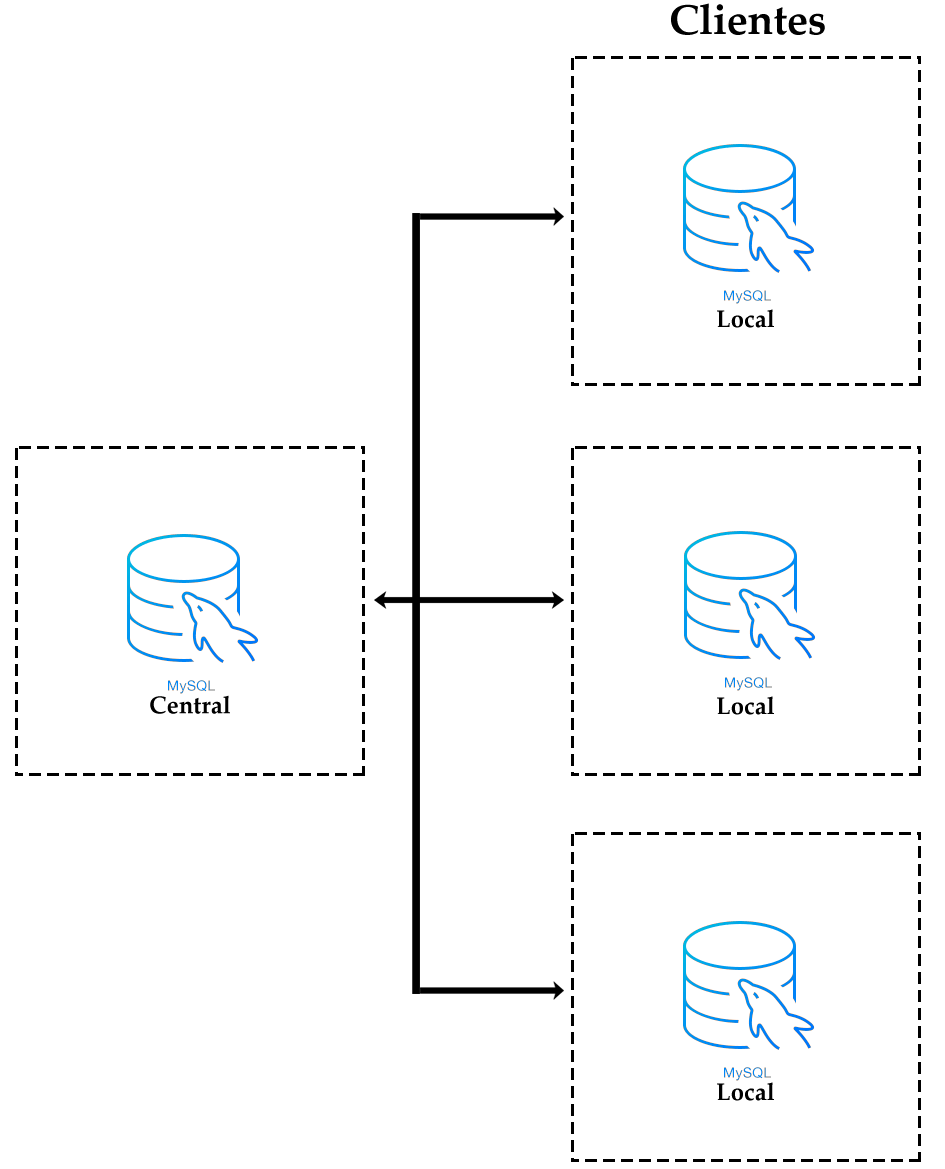
\includegraphics[width=0.40\textwidth]{Esquema_Projeto_4} % Include the image placeholder.png
		\caption[Diagrama das bases de dados]{Diagrama da infraestrutura com múltiplas BDs locais conectadas a uma BD central}
		\label{fig:infra1}
		\end{center}
\end{figure}
Para estabelecer o fluxo de informação desenvolveu-se um programa de transferência e um simulador, ambos desenvolvidos em \textit{C}. O programa de transferência envia \textit{queries} para as BDs locais e recebe respostas com registos que insere na BD central. O simulador gera registos para popular as BDs locais. Para simular múltiplos clientes usam-se simuladores independentes entre si, como representado na \autoref{fig:infra2}.
\begin{figure}[H]
	\begin{center}
		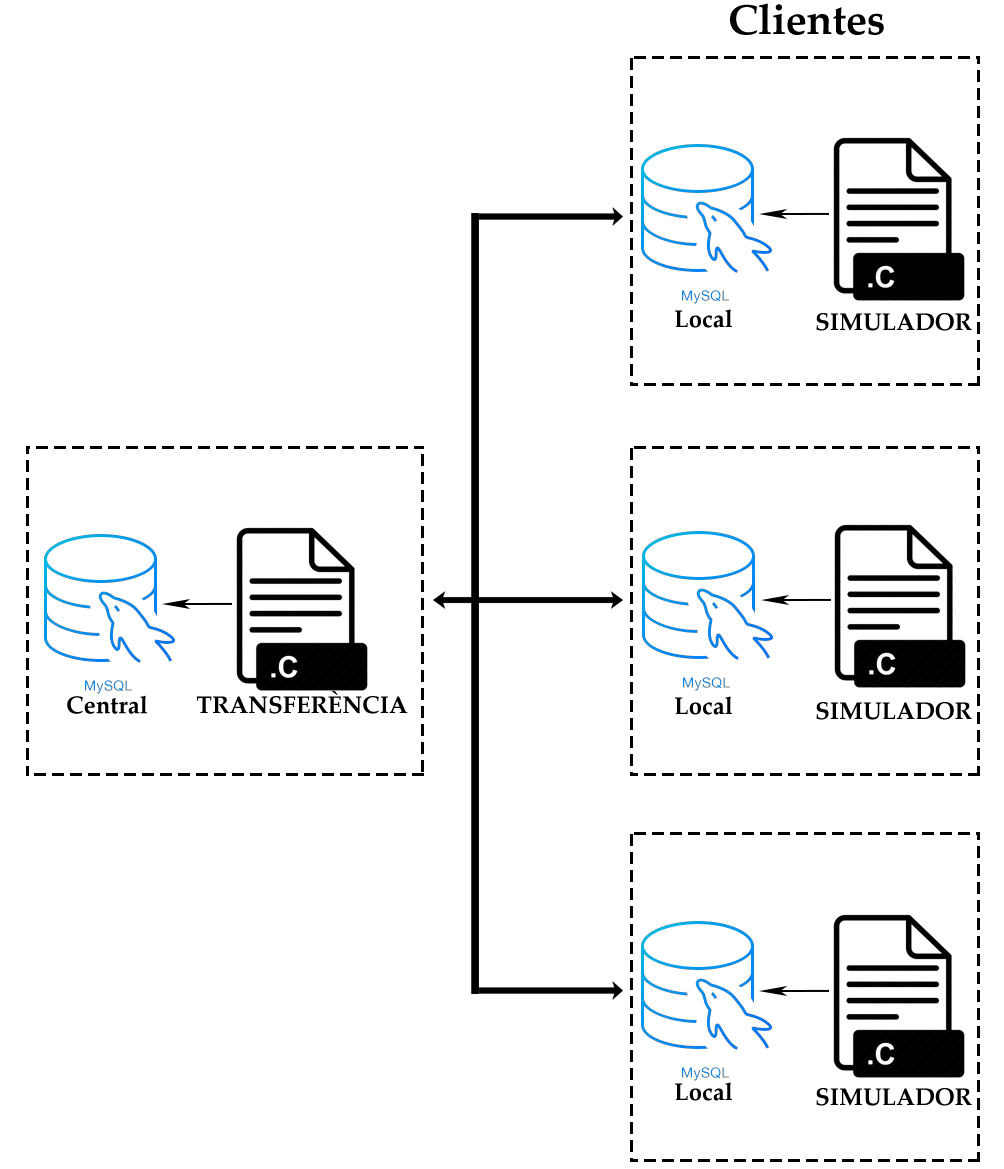
\includegraphics[width=0.55\textwidth]{Esquema_Projeto_5} % Include the image placeholder.png
		\caption[Diagrama do fluxo de informação]{Diagrama do fluxo de informação. Os simuladores substituem provisoriamente sistemas de aquisição de dados}
		\label{fig:infra2}
		\end{center}
\end{figure}
Para melhorar o desempenho da BD central e prevenir falhas críticas do sistema, desenvol-\\veu-se um programa de gestão de \textit{backups}, também em \textit{C}. Este programa limpa e cria \textit{backups} da BD e guarda-os num repositório \textit{online}. De forma a não interferir diretamente com a informação da BD central criam-se duas BDs para a gestão dos \textit{backups}. Com esta adição, o esquema da infraestrutura final está representado na \autoref{fig:infra3}.\par 
\begin{figure}
	\begin{center}
		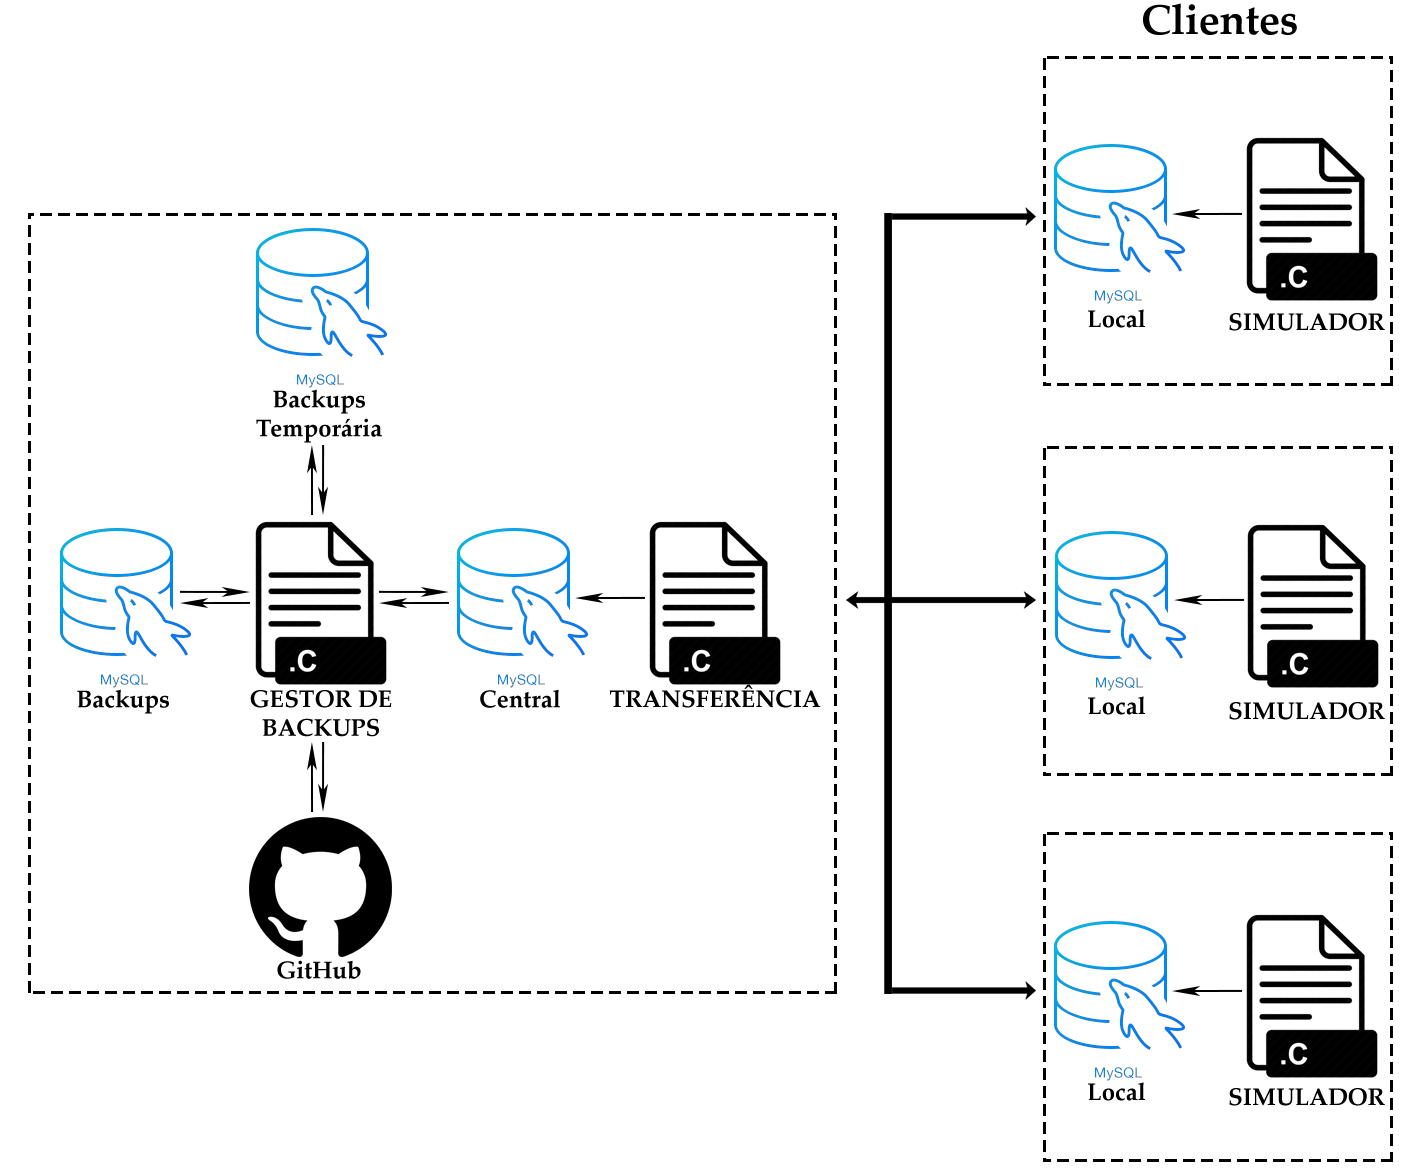
\includegraphics[width=1\textwidth]{Esquema_Projeto_6} % Include the image placeholder.png
		\caption[Diagrama final da infraestrutura]{Diagrama final da infraestrutura de dados. Os registos gerados nos simuladores são transferidos para a BD central. Estes registos são então processados pelo gestor de \textit{backups} que cria e guarda \textit{backups} provisoriamente num repositório online no \textit{GitHub}}
		\label{fig:infra3}
		\end{center}
\end{figure}

\section{Base de dados}
\subsection{Análise de requisitos}
\label{subchap:analise}
Deseja-se, de uma forma geral, um sistema capaz de guardar remotamente medições realizadas em moldes instrumentados. Esta informação não é suficiente para se deduzir uma base de dados. Assim sendo, analisando e completando a informação inicial chega-se ao seguinte enunciado:\par 
%\vspace{2ex}
\newpage
\textit{Um cliente, caracterizado por um ID único, nome, morada, IP e port, tem moldes. Estes moldes são identificados por um ID único, nome e descrição. Os moldes têm sensores com um número referente ao molde, tipo (termómetro, dinamómetro, extensómetro, etc.), nome e descrição. Estes sensores geram registos onde guardam a fase do processo (fecho do molde, enchimento, compactação, abertura e extração), data, hora, milissegundos e o valor num determinado momento.}\par 
\vspace{2ex}
Analisando este enunciado identificam-se as seguintes entidades com os seus respetivos atributos:
\begin{itemize}[noitemsep]
	\item Tipo
	\begin{itemize}[noitemsep]
		\item ID
		\item Nome
	\end{itemize}
	\item Fase
	\begin{itemize}[noitemsep]
		\item ID
		\item Nome
	\end{itemize}
	\item Clientes
	\begin{itemize}[noitemsep]
		\item ID de cliente único
		\item Nome
		\item Morada
		\item IP
		\item Port
	\end{itemize}
	\item Moldes
	\begin{itemize}[noitemsep]
		\item ID do cliente associado
		\item ID de molde único
		\item Nome
		\item Descrição
	\end{itemize}
	\item Sensores
	\begin{itemize}[noitemsep]
		\item ID do molde associado
		\item Número do sensor
		\item ID do tipo de sensor
		\item Nome
		\item Descrição
	\end{itemize}
	\item Registos
	\begin{itemize}[noitemsep]
		\item ID do molde associado
		\item Número do sensor associado
		\item ID da fase do processo
		\item Data
		\item Hora
		\item Milissegundos
		\item Valor
	\end{itemize}
\end{itemize}
\newpage
Analisando os atributos identificam-se as seguintes chaves primárias, únicas e estrangeiras:
\begin{itemize}[noitemsep]
	\item Tipo
	\begin{itemize}[noitemsep]
		\item Chave primária: ID
		\item Chaves únicas:
		\begin{enumerate}
			\item Nome
		\end{enumerate}
	\end{itemize}
	\item Fase
	\begin{itemize}[noitemsep]
		\item Chave primária: ID
		\item Chaves únicas:
		\begin{enumerate}
			\item Nome
		\end{enumerate}
	\end{itemize}
	\item Clientes
	\begin{itemize}[noitemsep]
		\item Chave primária: ID de cliente
	\end{itemize}
	\item Moldes
	\begin{itemize}[noitemsep]
		\item Chave primária: ID de molde
		\item Chaves estrangeiras:
		\begin{enumerate}
			\item ID do cliente associado
		\end{enumerate}
	\end{itemize}
	\item Sensores
	\begin{itemize}[noitemsep]
		\item Chave primária: ID do molde associado, Número do sensor
		\item Chaves estrangeiras:
		\begin{enumerate}
			\item ID do molde associado
			\item ID do tipo de sensor
		\end{enumerate}
	\end{itemize}
	\item Registos
	\begin{itemize}[noitemsep]
		\item Chave primária: ID do molde associado, Número do sensor associado, Data, Hora, Milissegundos
		\item Chaves estrangeiras:
		\begin{enumerate}
			\item ID do molde associado, Número do sensor associado
			\item ID da fase do processo
		\end{enumerate}
	\end{itemize}
\end{itemize}
O tipo de sensor e a fase do processo são dicionários ou seja, são entidades que contêm informação predefinida de forma a evitar a adição de dados incorretos nas entidades relacionadas. Os seus dados inicias são:
\begin{itemize}[noitemsep]
	\item Tipo
	\begin{itemize}[noitemsep]
		\item Termómetro
		\item Dinamómetro
		\item Extensómetro
		\item Vibrómetro
		\item Pressão
		\item Acelerómetro X
		\item Acelerómetro Y
		\item Acelerómetro Z
	\end{itemize}
	\newpage
	\item Fase
	\begin{itemize}[noitemsep]
		\item Fecho do molde
		\item Enchimento
		\item Compactação
		\item Abertura de molde
		\item Extração
	\end{itemize}
\end{itemize}
Ligando as várias entidades entre si identificam-se as seguintes relações com a respetiva cardinalidade:
\begin{itemize}[noitemsep]
	\item 1 cliente tem muitos moldes (1 para N)
	\item 1 molde tem muitos sensores (1 para N)
	\item 1 sensor tem muitos registos (1 para N)
	\item 1 tipo define muitos sensores (1 para N)
	\item 1 fase define muitos registos (1 para N)
\end{itemize}
Quanto à obrigatoriedade de participação das entidades nas relações anteriores afirma-se:
\begin{itemize}[noitemsep]
	\item Não pode existir moldes sem clientes
	\item Não pode existir sensores sem moldes
	\item Não pode existir registos sem sensores
	\item Não pode existir sensores sem tipo
	\item Não pode existir registos sem fase	
\end{itemize}

\subsection{Diagrama Entidade/Relação e Esquema Relacional}
Concatenando a informação descrita na análise de requisitos, obtém-se o DER representado na \autoref{fig:der}. No \autoref{apen:DER} encontra-se um histórico dos DERs realizados durante o desenvolvimento do projeto\par
\newpage
\begin{landscape}
	\begin{figure}
		\begin{center}
			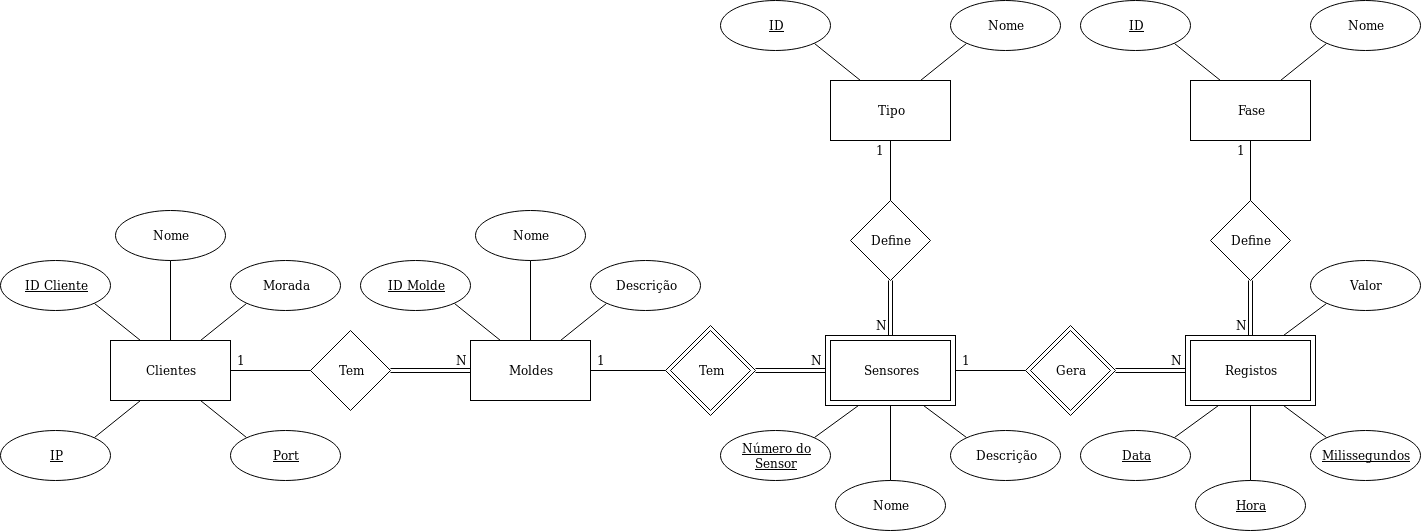
\includegraphics[width=1.4\textwidth]{diagrama_entidade_relacao} % Include the image placeholder.png
			\caption[Diagrama Entidade/Relação final do projeto]{Diagrama Entidade/Relação final do projeto realizado a partir da análise de requisitos}
			\label{fig:der}
		\end{center}
	\end{figure}
\end{landscape}
Traduzindo as entidades do diagrama anterior para tabelas e as relações para chaves estrangeiras, obtém-se o esquema lógico da BD representado na \autoref{fig:er}.
\begin{figure}[H]
	\begin{center}
		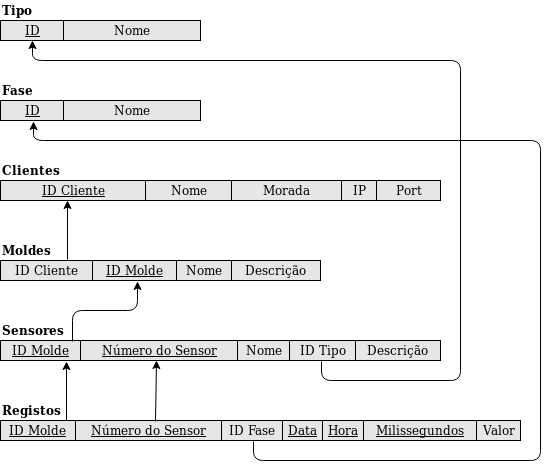
\includegraphics[width=1\textwidth]{esquema_relacional} % Include the image placeholder.png
		\caption[Esquema Lógico final do projeto]{Esquema Lógico final do projeto obtido através da análise do DER na \autoref{fig:der} onde as entidades e os seus atributos se traduzem em tabelas e as relações nas chaves estrangeiras destas}
		\label{fig:er}
	\end{center}
\end{figure}

\newpage
\subsection{Construção da base de dados}
Avançando para a criação das tabelas em \textit{MySQL}, a fim de evitar ambiguidades no nome dos atributos estes são alterados para campos semânticos específicos a cada entidade. Para cada atributo define-se o domínio e a obrigatoriedade como representado na \autoref{tab:dominio}.
\begin{table}[H]
	\centering
	\begin{tabular}{|l|l|l|l|l|l|}
		%\hline
		\multicolumn{6}{l}{\textbf{tipo}}\\ \cline{1-2}
		tipo\texttt{\char`_}ID & tipo\texttt{\char`_}nome & \multicolumn{4}{l}{}\\ \cline{1-2}
		int & varchar(50) & \multicolumn{4}{l}{}\\ \cline{1-2}
		not null & not null & \multicolumn{4}{l}{}\\ \cline{1-2}
		\multicolumn{6}{l}{\textbf{fase}}\\ \cline{1-2}
		fase\texttt{\char`_}ID & fase\texttt{\char`_}nome & \multicolumn{4}{l}{}\\ \cline{1-2}
		int & varchar(50) & \multicolumn{4}{l}{}\\ \cline{1-2}
		not null & not null & \multicolumn{4}{l}{}\\ \cline{1-2}
		\multicolumn{6}{l}{\textbf{clientes}}\\ \cline{1-5}
		cl\texttt{\char`_}ID & cl\texttt{\char`_}nome & cl\texttt{\char`_}morada & cl\texttt{\char`_}IP & cl\texttt{\char`_}port & \multicolumn{1}{l}{}\\ \cline{1-5}
		int & varchar(50) & varchar(100) & varchar(50) & int & \multicolumn{1}{l}{}\\ \cline{1-5}
		not null & not null & & not null & not null & \multicolumn{1}{l}{}\\ \cline{1-5}
		\multicolumn{6}{l}{\textbf{moldes}}\\ \cline{1-4}
		m\texttt{\char`_}IDCliente & m\texttt{\char`_}ID & 
		m\texttt{\char`_}nome & 
		m\texttt{\char`_}descricao & \multicolumn{2}{l}{}\\ \cline{1-4}
		int & int & varchar(30) & varchar(200) & \multicolumn{2}{l}{}\\ \cline{1-4}
		not null & not null & & &  \multicolumn{2}{l}{}\\ \cline{1-4}
		\multicolumn{6}{l}{\textbf{sensores}}\\ \cline{1-5}
		s\texttt{\char`_}IDMolde & s\texttt{\char`_}num & s\texttt{\char`_}tipo & s\texttt{\char`_}nome & s\texttt{\char`_}descricao & \multicolumn{1}{l}{}\\ \cline{1-5}
		int & int & int & varchar(30) & varchar(200) & \multicolumn{1}{l}{}\\ \cline{1-5}
		not null & not null & not null & & & \multicolumn{1}{l}{}\\ \cline{1-5}
		\multicolumn{6}{l}{\textbf{registos}}\\ \hline
		r\texttt{\char`_}IDMolde & r\texttt{\char`_}numSensor & r\texttt{\char`_}fase &  r\texttt{\char`_}data\texttt{\char`_}hora & r\texttt{\char`_}milissegundos & r\texttt{\char`_}valor\\ \hline
		int & int & int & datetime & tinyint & float\\ \hline
		not null & not null & not null & not null & not null & \\ \hline
	\end{tabular}
	\caption[Tabelas da BD com os seus atributos e respetivos domínios e obrigatoriedades]{Tabelas da BD com os seus atributos e respetivos domínios e obrigatoriedades. Os atributos data e hora da entidade registos são fundidos no atributo r\texttt{\char`_}data\texttt{\char`_}hora graças ao tipo de dados \texttt{datetime}}
	\label{tab:dominio}
\end{table}
Define-se então nomes para as restrições de integridade definidas pelas chaves das entidades:
\begin{itemize}[noitemsep]
	\item Tipo
	\begin{itemize}[noitemsep]
		\item Restrição chave primária: REPETIDO\texttt{\char`_}ID\texttt{\char`_}TIPO
		\item Restrição chaves únicas:
		\begin{enumerate}
			\item REPETIDO\texttt{\char`_}NOME\texttt{\char`_}TIPO
		\end{enumerate}
	\end{itemize}
	\item Fase
	\begin{itemize}[noitemsep]
		\item Restrição chave primária: REPETIDO\texttt{\char`_}ID\texttt{\char`_}FASE
		\item Restrição chaves únicas:
		\begin{enumerate}
			\item REPETIDO\texttt{\char`_}NOME\texttt{\char`_}FASE
		\end{enumerate}
	\end{itemize}
	\item Clientes
	\begin{itemize}[noitemsep]
		\item Restrição chave primária: REPETIDO\texttt{\char`_}ID\texttt{\char`_}CLIENTE
	\end{itemize}
	\item Moldes
	\begin{itemize}[noitemsep]
		\item Restrição chave primária: REPETIDO\texttt{\char`_}ID\texttt{\char`_}MOLDE
		\item Restrição chaves estrangeiras:
		\begin{enumerate}
			\item MOLDE\texttt{\char`_}MAU\texttt{\char`_}ID\texttt{\char`_}CLIENTE
		\end{enumerate}
	\end{itemize}
	\item Sensores
	\begin{itemize}[noitemsep]
		\item Restrição chave primária: REPETIDO\texttt{\char`_}NUM\texttt{\char`_}SENSOR
		\item Restrição chaves estrangeiras:
		\begin{enumerate}
			\item SENSOR\texttt{\char`_}MAU\texttt{\char`_}ID\texttt{\char`_}MOLDE
			\item SENSOR\texttt{\char`_}MAU\texttt{\char`_}ID\texttt{\char`_}TIPO
		\end{enumerate}
	\end{itemize}
	\item Registos
	\begin{itemize}[noitemsep]
		\item Restrição chave primária: REPETIDO\texttt{\char`_}REGISTO
		\item Restrição chaves estrangeiras:
		\begin{enumerate}
			\item REGISTOS\texttt{\char`_}MAU\texttt{\char`_}ID\texttt{\char`_}MOLDE\texttt{\char`_}SENSOR
			\item REGISTOS\texttt{\char`_}MAU\texttt{\char`_}ID\texttt{\char`_}FASE
		\end{enumerate}
	\end{itemize}
\end{itemize}
Em relação ao comportamento das restrições das chaves estrangeiras identificam-se as seguintes opções:
\begin{itemize}
	\item ON DELETE NO ACTION ON UPDATE NO ACTION
	\begin{itemize}
		\item MOLDE\texttt{\char`_}MAU\texttt{\char`_}ID\texttt{\char`_}CLIENTE
		\item SENSOR\texttt{\char`_}MAU\texttt{\char`_}ID\texttt{\char`_}TIPO
		\item REGISTOS\texttt{\char`_}MAU\texttt{\char`_}ID\texttt{\char`_}FASE
	\end{itemize}
	\item ON DELETE CASCADE ON UPDATE NO ACTION
	\begin{itemize}
		\item SENSOR\texttt{\char`_}MAU\texttt{\char`_}ID\texttt{\char`_}MOLDE
		\item REGISTOS\texttt{\char`_}MAU\texttt{\char`_}ID\texttt{\char`_}MOLDE\texttt{\char`_}SENSOR
	\end{itemize}
\end{itemize}
Estes comportamentos definem que quando se tenta atualizar a chave primária de um tuplo (\textit{UPDATE}), se esta tiver tuplos associados a ela, a operação não deve ser realizada pois pode comprometer os dados existentes na BD. No entanto, quando se tenta eliminar um tuplo são definidos dois comportamentos. Como existe muita informação associada a cada cliente, como segurança, não se permite a eliminação de um tuplo desta tabela, se este tiver informação associada a si noutras tabelas. O mesmo se aplica aos dicionários, se se tentar eliminar um tuplo, a informação associada não deve ser comprometida. No caso dos registos, dado que estão associados diretamente a um molde, se um tuplo da tabela moldes for eliminado, os dados dos seus sensores e respetivos registos devem ser também eliminados para manter a BD limpa e sem informação desnecessária.\par 
\newpage
Revendo as restrições de integridade criadas pelas chaves estrangeiras, como não se pode criar uma tabela que dependa de outra que não tenha sido ainda criada, define-se uma ordem para a criação das tabelas:
\begin{enumerate}[noitemsep]
	\item Tipo
	\item Fase
	\item Clientes
	\item Moldes
	\item Sensores
	\item Registos
\end{enumerate}
Este modelo de dados aplica-se a todas as BDs usadas neste projeto com a exceção da BD regulação de procedimentos abordada na \autoref{subchap:notificacoes} e temporária local abordada na \autoref{subchap:adap}.

\subsection{Base de dados regulação de procedimentos}
\label{subchap:notificacoes}
Com a introdução da aplicação de gestão do sistema surge a necessidade desta comunicar com os programas de transferência e gestão de \textit{backups}. Para este efeito cria-se a BD regulação de procedimentos, com a qual a aplicação comunica de forma a ditar o modo de funcionamento dos programas, como representado na \autoref{fig:infra4}. Na \autoref{fig:infra_total1} está representada a infraestrutura completa com todas as bases de dados numa utilização a baixo nível.
\begin{figure}[H]
	\centering
	\begin{center}
		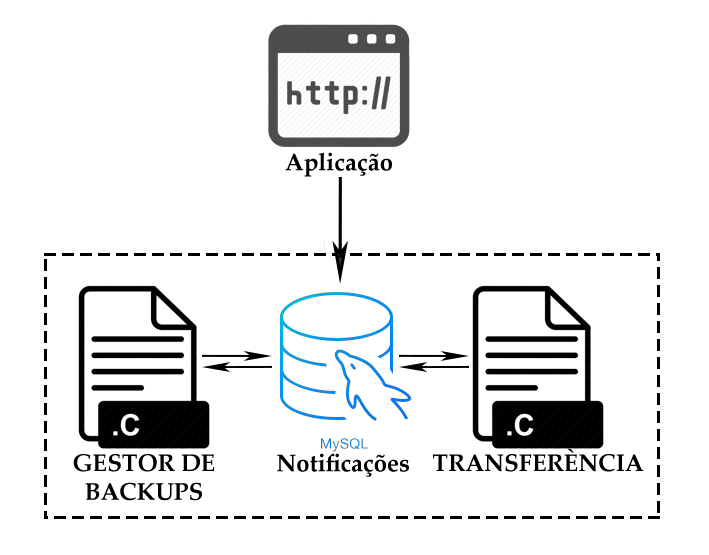
\includegraphics[width=0.5\textwidth]{Aplicacao_notificacoes} % Include the image placeholder.png
		\caption[Diagrama da comunicação com a base de dados regulação de procedimentos]{Diagrama da comunicação com a BD regulação de procedimentos, onde os programas de transferência e gestão de \textit{backups} verificam parâmetros introduzidos pela aplicação de gestão do sistema}
		\label{fig:infra4}
	\end{center}
\end{figure}
Esta BD contém variáveis globais importantes para a comunicação entre a aplicação e os programas. Define-se as entidades com os seus atributos e respetivos domínios e obrigatoriedade, como representado na \autoref{tab:notificacoes}. As entidades não se relacionam entre e por isso esta BD não se classifica como uma BD relacional. No entanto, utilizam-se os mesmos termos para descrever o desenvolvimento desta.
\begin{figure}
	\begin{center}
		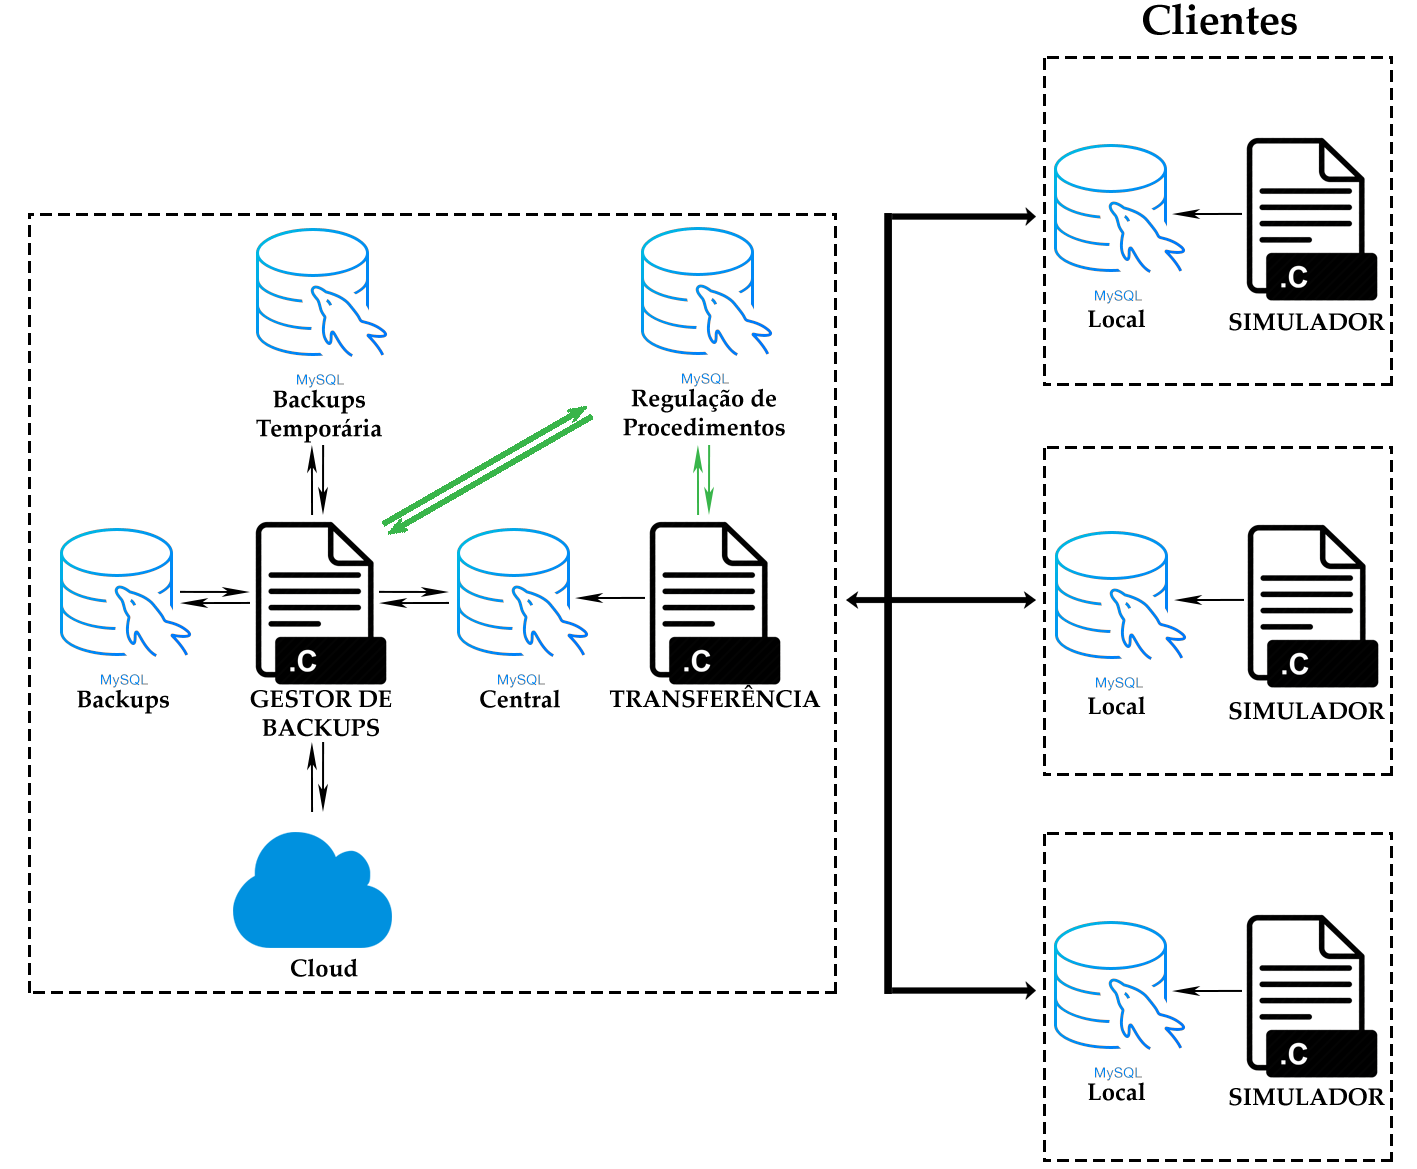
\includegraphics[width=1\textwidth]{Esquema_Projeto_Total01} % Include the image placeholder.png
		\caption[Diagrama da infraestrutura completa sem aplicação de gestão do sistema]{Diagrama da infraestrutura completa, numa utilização de baixo nível, sem aplicação de gestão do sistema. A preto está representado o fluxo de registos e a verde o fluxo de regulação de procedimentos}
		\label{fig:infra_total1}
	\end{center}
\end{figure}
\newpage
\begin{table}
	\centering
	\begin{tabular}{|l|l|l|}
		%\hline
		\multicolumn{3}{l}{\textbf{atualizar}}\\ \cline{1-3}
		a\texttt{\char`_}indice & a\texttt{\char`_}transferencia & a\texttt{\char`_}backups\\ \cline{1-3}
		int & int & int\\ \cline{1-3}
		not null & not null & not null\\ \cline{1-3}
		\multicolumn{3}{l}{\textbf{backups}}\\ \cline{1-1}
		b\texttt{\char`_}IDMolde &\multicolumn{2}{l}{}\\ \cline{1-1}
		int &\multicolumn{1}{l}{}\\ \cline{1-1}
		 &\multicolumn{2}{l}{}\\ \cline{1-1}
	\end{tabular}
	\caption[Tabelas da base de dados regulação de procedimentos com os seus atributos e respetivos domínios e obrigatoriedades]{Tabela BD regulação de procedimentos com os seus atributos e respetivos domínios e obrigatoriedades}
	\label{tab:notificacoes}
\end{table}
\newpage
A tabela Atualizar só deve ter um tuplo, considera-se o atributo \texttt{a\char`_indice} como chave primária que só pode ser igual a 1 e os atributos \texttt{a\char`_transferencia} e \texttt{a\char`_backups} só devem ser igual a 0 ou 1. Assim sendo definem-se as restrições:
\begin{itemize}[noitemsep]
	\item Atualizar
	\begin{itemize}[noitemsep]
		\item Restrição chave primária:
		\begin{enumerate}
			\item REPETIDO\texttt{\char`_}INDICE\texttt{\char`_}ATUALIZAR
		\end{enumerate}
		\item Restrição valor:
		\begin{enumerate}
			\item ATUALIZAR{\char`_}MAU\texttt{\char`_}VALOR\texttt{\char`_}INDICE
			\item ATUALIZAR{\char`_}MAU\texttt{\char`_}VALOR\texttt{\char`_}TRANSFERENCIA
			\item ATUALIZAR{\char`_}MAU\texttt{\char`_}VALOR\texttt{\char`_}BACKUPS
		\end{enumerate}
	\end{itemize}
	\item Backups
	\begin{itemize}[noitemsep]
		\item Restrição chave primária:
		\begin{enumerate}
			\item REPETIDO\texttt{\char`_}ID\texttt{\char`_}MOLDE
		\end{enumerate}
	\end{itemize}
\end{itemize}
Define-se que tabela Atualizar deve ser iniciada com um tuplo com \texttt{a\char`_indice} igual a 1, \texttt{a\char`_transferencia} igual a 0 e \texttt{a\char`_backups} igual a 0. As funcionalidades desta BD são exploradas nas Subsecções \ref{subchap:transferencia} e \ref{subchap:backups}.

\section{Programa de transferência}
\label{subchap:transferencia}
Este programa prioriza a conservação dos registos e a sua taxa de transferência. O código foi realizado com vista à portabilidade para outras linguagens de programação. Consiste em várias ideias simples que podem ser observadas de forma reduzida nas Figuras \ref{fig:transferencia_simples_programa} e \ref{fig:transferencia_simples_subprograma}. As versões completas destes fluxogramas podem ser encontradas no \autoref{apen:fluxogramas}.\par
\begin{figure}
	%\vspace{-3cm}
	\begin{center}
		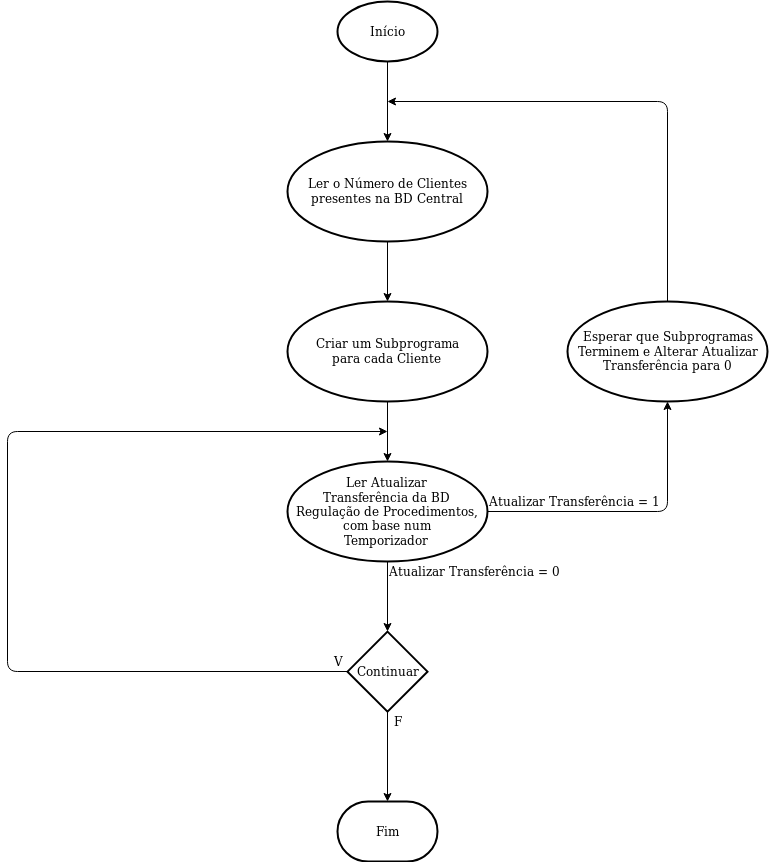
\includegraphics[width=1\textwidth]{fluxograma_simples_transferencia_programa01} % Include the image placeholder.png
		%\vspace{9cm}
		\caption[Fluxograma reduzido do programa principal de transferência]{Fluxograma reduzido do programa principal de transferência, que cria subprogramas}
		\label{fig:transferencia_simples_programa}
	\end{center}
\end{figure}
\begin{figure}
	\vspace{-0.5cm}
	\begin{center}
		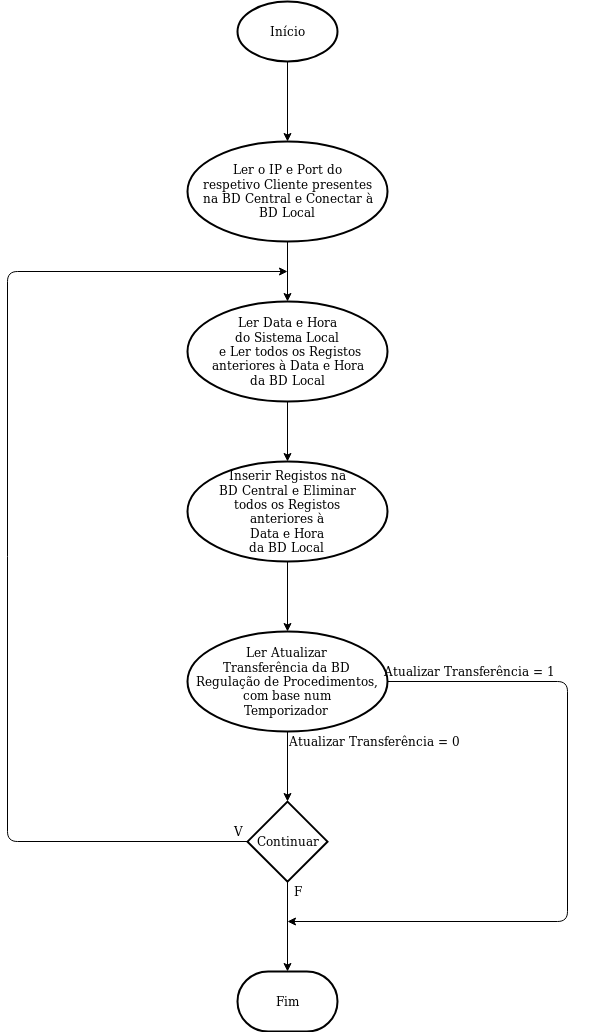
\includegraphics[width=0.8\textwidth]{fluxograma_simples_transferencia_subprograma01} % Include the image placeholder.png
		\caption[Fluxograma reduzido dos subprogramas de transferência]{Fluxograma reduzido dos subprogramas de transferência, que transferirem os registos de cada cliente para a BD central}
		\label{fig:transferencia_simples_subprograma}
	\end{center}
\end{figure}
Seguindo a estrutura do programa, primeiramente realiza-se uma conexão à BD central, seguida de uma \textit{query} para se saber o número de clientes existentes:
\begin{lstlisting}[language = SQL]
	SELECT *
	FROM central.clientes;
\end{lstlisting}
Guarda-se o número de tuplos retornados numa variável e termina-se a conexão à BD central. De seguida replica-se o programa múltiplas vezes até se ter um subprograma para cada cliente com recurso à função:
\begin{lstlisting}[language = C]
	fork();
\end{lstlisting}
Atribui-se a cada subprograma o número do cliente a que está associado. Cada um realiza uma conexão à BD central e obtém os respetivos \textit{IPs} e \textit{ports}, necessários para realizar a conexão à BD local do cliente a que está associado:
\begin{lstlisting}[language = SQL]
	SELECT cl_ID, cl_IP, cl_port
	FROM central.clientes
	ORDER BY cl_ID;
\end{lstlisting}
Com as conexões central e local estabelecidas inicia-se um ciclo infinito para a transferência de valores. Com a \textit{query} à BD local:
\begin{lstlisting}[language = SQL]
	SELECT CURRENT TIMESTAMP;
\end{lstlisting}
Recebe-se a data e hora atual do sistema local e guarda-se numa variável \texttt{@datahora\char`_lim}. De seguida obtém-se todos os registos anteriores à data e hora:
\begin{lstlisting}[language = SQL]
	SELECT *
	FROM local.registos
	WHERE r_data_hora < @datahora_lim
	ORDER BY r_data_hora, r_milissegundos,
	r_numSensor, r_IDMolde;
\end{lstlisting}
Esta organização pela data e hora garante uma transferência uniforme de valores. Por predefinição, o sistema retorna os registos de um sensor de cada vez, tornando a transferência de valores menos eficiente para efeitos de análise. Por outras palavras, prefere-se saber os registos de todos os sensores num dado instante do que todos os registos de um sensor até ao momento.\par 
Os tuplos retornados são guardados numa \textit{string} \texttt{@resposta} e inseridos na BD central com uma \textit{query} do tipo:
\begin{lstlisting}[language = SQL]
	INSERT IGNORE central.registos VALUES
	(tuplo1),
	(tuplo2),
	(tuplo3),
	...,
	(tuploN);
\end{lstlisting}
Inserir múltiplos tuplos permite uma maior taxa de transferência comparativamente a uma inserção individual. A \textit{string} \texttt{@resposta} tem uma dimensão limitada, se a resposta proveniente da BD local for superior ao tamanho da variável, o programa divide-a em grupos de informação mais pequenos que respeitem a dimensão desta variável. Explicando melhor com um exemplo: se forem retornados 500 tuplos e a capacidade de \texttt{@resposta} for de 100 tuplos, divide-se a informação em 5 repostas.\par 
A escolha da opção \texttt{IGNORE} garante que não são perdidos registos, no caso de serem gerados registos repetidos ou não válidos. Após a transferência ser concluída, os tuplos transferidos da BD local são eliminados:
\begin{lstlisting}[language = SQL]
	DELETE FROM local.registos
	WHERE r_data_hora < @datahora_lim;
\end{lstlisting}
Sempre que se desejar um subprograma para um cliente novo, o programa de transferência deve ser reiniciado. Isto pode ser realizado manualmente ou atualizando o valor de \texttt{a\char`_transferencia} para 1. Com base num temporizador o programa principal e os subprogramas realizam a \textit{query} à BD regulação de procedimentos:
\begin{lstlisting}[language = SQL]
	SELECT a_transferencia
	FROM reg_proc.atualizar
	WHERE a_indice = 1;
\end{lstlisting}
Se \texttt{@a\char`_transferencia} for igual a 1, os subprogramas terminam após completarem os seus ciclos e o programa principal recomeça do principio e altera este parâmetro para 0, como demonstrado nas Figuras \ref{fig:transferencia_simples_programa} e \ref{fig:transferencia_simples_subprograma}:
\begin{lstlisting}[language = SQL]
	UPDATE reg_proc.atualizar
	SET a_transferencia = 0
	WHERE a_indice = 1;
\end{lstlisting}

\section{Gestão de \textit{backups}}
\label{subchap:backups}
À semelhança do programa anterior, o programa de gestão de \textit{backups} foi realizado com vista à portabilidade para outras linguagens de programação. Este programa está dividido nas componentes de gerar e concatenar \textit{backups}.\par 
A primeira serve para manter a informação armazenada organizada. Gera \textit{backups} segmentados dos históricos de registos da BD central e depois elimina a informação já salvaguardada. Isto aumenta a velocidade da consulta de registos mais recentes e previne que a base de dados central exceda o limite de 4Gb impostos pela versão gratuita do \textit{MySQL}, como referido na \autoref{subchap:mysql}. Em vez de se gerar um \textit{backup} de toda a base de dados, gera-se um \textit{backup} específico para cada molde, que inclui a informação dos seus sensores, registos e cliente a que está associado. Além destes, realiza-se um outro \textit{backup} com a informação dos clientes, moldes e sensores mais atual. Assim, em caso de falha crítica, simplifica-se a recuperação do sistema.\par 
A segunda serve para concatenar os \textit{backups} segmentados, produzidos durante o tempo de funcionamento de um molde, num \textit{backup} total do histórico de registos deste molde. Quando um molde sai de produção pode ser interessante arquivar o seu histórico e esta ação pode ser facilitada se, em vez de serem arquivados dezenas ou centenas de \textit{backups}, for apenas arquivado um \textit{backup} geral com todo o histórico do molde.\par 
Ao contrário do programa anterior, este não executa de forma contínua. Define-se um temporizador para executar cada componente. Utilizam-se temporizadores diferentes: o temporizador para gerar \textit{backups} e o temporizador para concatenar \textit{backups}. O temporizador para gerar \textit{backups} fica associado à primeira componente, esta executa automaticamente e em intervalos espaçados. Por exemplo, podem ser gerados \textit{backups} uma vez por dia ou uma vez por semana ou uma vez por mês dependendo da quantidade de informação produzida. O temporizador para concatenar \textit{backups} fica associado à segunda componente, esta deve executar quando o utilizador deseja e deve garantir uma resposta do programa com a menor latência possível.
As Figuras \ref{fig:backups_simples_programa}, \ref{fig:backups_simples_gerar} e \ref{fig:backups_simples_concatenar} representam de forma reduzida a estrutura do programa. As versões completas destes fluxogramas podem ser encontradas no \autoref{apen:fluxogramas}.\par 
\begin{figure}
	\begin{center}
		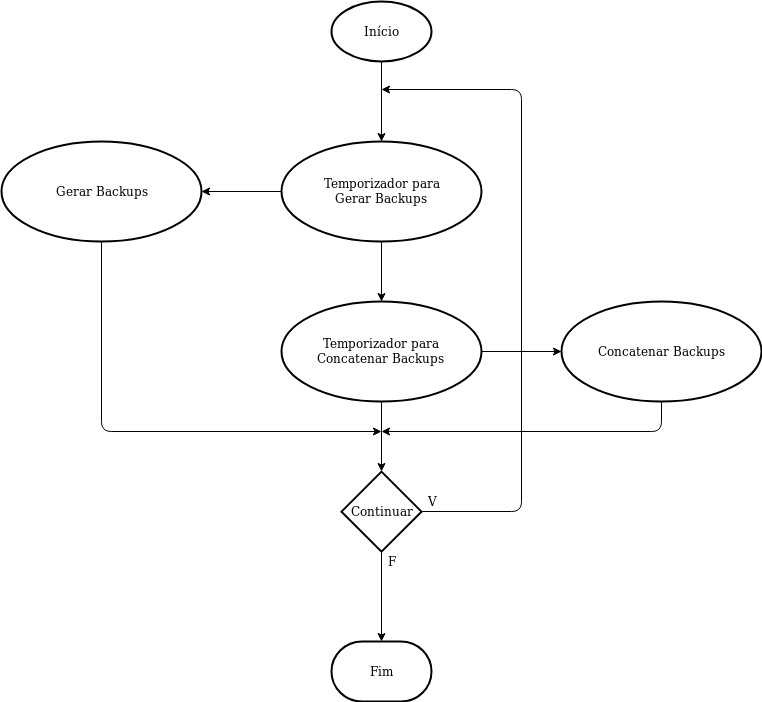
\includegraphics[width=1\textwidth]{fluxograma_simples_backups_programa01} % Include the image placeholder.png
		\caption[Fluxograma reduzido do programa principal de \textit{backups}]{Fluxograma reduzido do programa principal de \textit{backups}, com os temporizadores para gerar ou concatenar \textit{backups}}
		\label{fig:backups_simples_programa}
	\end{center}
\end{figure}
\begin{figure}
	\begin{center}
		\hspace{3.5cm}
		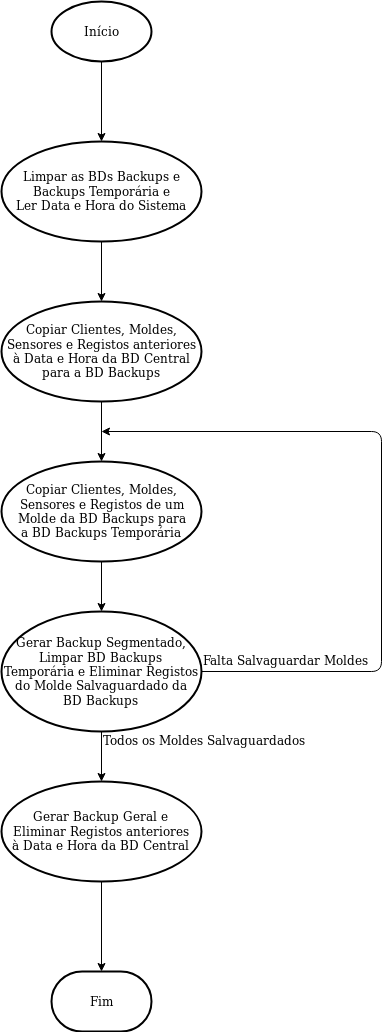
\includegraphics[width=0.5\textwidth]{fluxograma_simples_backups_gerar01} % Include the image placeholder.png
		\caption[Fluxograma reduzido da componente de gerar \textit{backups}]{Fluxograma reduzido da componente de gerar \textit{backups}. Quando esta chega ao fim retorna ao ciclo do programa principal representado na \autoref{fig:backups_simples_programa}}
		\label{fig:backups_simples_gerar}
	\end{center}
\end{figure}
\begin{figure}
	\begin{center}
		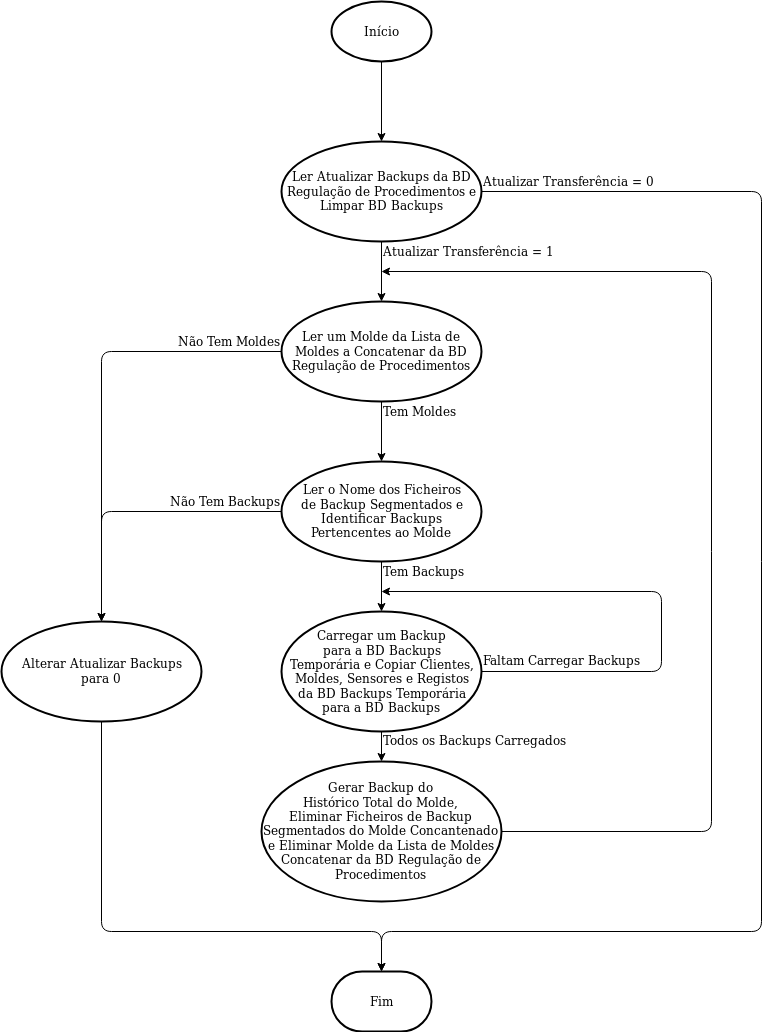
\includegraphics[width=1\textwidth]{fluxograma_simples_backups_concatenar01} % Include the image placeholder.png
		\caption[Fluxograma reduzido da componente de concatenar \textit{backups}]{Fluxograma reduzido da componente de concatenar \textit{backups}. Quando esta chega ao fim retorna ao ciclo do programa principal representado na \autoref{fig:backups_simples_programa}}
		\label{fig:backups_simples_concatenar}
	\end{center}
\end{figure}
\newpage
Seguindo a estrutura da componente de geração de \textit{backups} representada na \autoref{fig:backups_simples_gerar}, realizam-se as conexões às BDs central, \textit{backups} e \textit{backups} temporária. Realiza-se então uma limpeza das BDs \textit{backups} e \textit{backups} temporária para certificar que não existem valores residuais que possam comprometer a informação dos \textit{backups}:
\begin{lstlisting}[language = SQL]
	DELETE FROM backups.moldes;
	DELETE FROM backups.clientes;
	DELETE FROM backups_temp.moldes;
	DELETE FROM backups_temp.clientes;
\end{lstlisting}
Com a \textit{query}:
\begin{lstlisting}[language = SQL]
	SELECT CURRENT TIMESTAMP;
\end{lstlisting}
Recebe-se a data e hora atual do sistema e guarda-se numa variável \texttt{@datahora\char`_lim}. Para proteger os dados presentes na BD central, realiza-se a cópia dos registos para a BD \textit{backups}:
\begin{lstlisting}[language = SQL]
	INSERT IGNORE backups.clientes
	SELECT *
	FROM central.clientes;
	INSERT IGNORE backups.moldes
	SELECT *
	FROM central.moldes;
	INSERT IGNORE backups.sensores
	SELECT *
	FROM central.sensores;
	INSERT IGNORE backups.registos
	SELECT *
	FROM central.registos
	WHERE r_data_hora < @datahora_lim;
\end{lstlisting}
De forma a gerar um \textit{backup} para cada molde filtra-se a informação com base no seu ID:
\begin{lstlisting}[language = SQL]
	SELECT m_IDCliente, m_ID
	FROM backups.moldes;
\end{lstlisting}
As respostas são guardadas nas variáveis \texttt{@IDCliente} e \texttt{@IDMolde}. De forma cíclica copia-se a informação para a BD \textit{backups} temporária:
\begin{lstlisting}[language = SQL]
	INSERT IGNORE backups_temp.clientes
	SELECT *
	FROM backups.clientes
	WHERE cl_ID = @IDCliente;
	INSERT IGNORE backups_temp.moldes
	SELECT *
	FROM backups.moldes
	WHERE m_ID = @IDMolde;
	INSERT IGNORE backups_temp.sensores
	SELECT *
	FROM backups.sensores
	WHERE m_ID = @IDMolde;
	INSERT IGNORE backups_temp.registos
	SELECT *
	FROM backups.registos
	WHERE m_ID = @IDMolde;
\end{lstlisting}
Após os valores copiados retiram-se informações sobre a data e hora mais antiga e mais recente:
\begin{lstlisting}[language = SQL]
	SELECT r_data_hora
	FROM backups_temp.registos
	ORDER BY r_data_hora
	LIMIT 1;
	SELECT r_data_hora
	FROM backups_temp.registos
	ORDER BY r_data_hora DESC
	LIMIT 1;
\end{lstlisting}
Os valores retornados são guardados nas variáveis \texttt{@dataIni} e \texttt{@dataFim}. Com estes valores e com a função:
\begin{lstlisting}[language = C]
	FILE *popen(const char *command, const chat *mode);
\end{lstlisting}
Envia-se para o terminal o comando que gera os \textit{backups} num local predefinido:
\begin{lstlisting}[language = bash]
	mysqldump -u backupmanager -pbackup1234 backups_temp >
	~/Backups/backup_@IDCliente_@IDMolde_@dataIni_@dataFim.sql
\end{lstlisting}
Depois do ficheiro ser criado com sucesso elimina-se das BDs \textit{backups} e \textit{backups} temporária a informação relativa ao molde:
\begin{lstlisting}[language = SQL]
	DELETE FROM backups_temp.moldes;
	DELETE FROM backups_temp.clientes;
	DELETE FROM bakups.registos
	WHERE r_IDMolde = @IDMolde;
\end{lstlisting}
Quando todos os moldes tiverem sido armazenados, a tabela registos da BD \textit{backups} deve estar vazia. Realiza-se então o \textit{backup} da restante informação dos clientes, moldes, sensores, tipo e fase para efeitos de recuperação do sistema:
\begin{lstlisting}[language = bash]
	mysqldump -u backupmanager -pbackup1234 backups_temp >
	~/Backups/backup_geral.sql
\end{lstlisting}
Definiu-se um nome estático para este \textit{backup}. Este será rescrito cada vez que o programa executa enquanto os \textit{backups} individuais dos moldes vão acumulando com o tempo. Termina-se o processo apagando os valores armazenados na BD central:
\begin{lstlisting}[language = SQL]
	DELETE FROM central.registos
	WHERE r_data_hora < @datahora_lim;
\end{lstlisting}
Os \textit{backups} são então transferidos para o repositório \textit{online} no \textit{GitHub}. Esta solução serve apenas para demonstrar a capacidade de mover os \textit{backups} para um sistema diferente. Do ponto de vista prático, não se recomenda guardar informação potencialmente sensível num servidor público.\par 
Na eventualidade de surgir uma falha crítica no sistema central, e este necessitar de ser formatado ou substituído, os registos cessarão de ser transferidos dos sistemas locais. Isto não significa que a informação esteja comprometida, apenas não está a ser transferida. Após re-instalar utiliza-se manualmente no terminal o comando:
\begin{lstlisting}[language = bash]
	mysql -u backupmanager -pbackup1234 central <
	~/Backups/backup_geral.sql
\end{lstlisting}
Isto faz com que se recupere a informação dos clientes, moldes e sensores presentes no último \textit{backup} geral mais rapidamente acelerando o processo de restauro, comparativamente a uma inserção manual dos dados.\par 
Passando para a componente de concatenação de \textit{backups}, os ficheiros criados com o comando \texttt{mysqldump} contêm toda a informação das tabelas e funcionam como ponto de restauro. Isto significa que quando se usa o comando de recuperação, a BD selecionada é substituída pela que está no ficheiro \texttt{.sql}. Este comportamento dificulta a concatenação de vários \textit{backups} numa única BD. Assim sendo, à semelhança da primeira componente, utiliza-se a BD \textit{backups} temporária como BD intermédia para a concatenação de \textit{backups}.\par 
Seguindo a estrutura do programa representada na \autoref{fig:backups_simples_concatenar}, realizam-se as conexões às BDs central, \textit{backups}, \textit{backups} temporária e regulação de procedimentos. Com a \textit{query}:
\begin{lstlisting}[language = SQL]
	SELECT a_backups
	FROM reg_proc.atualizar
	WHERE a_indice = 1;
\end{lstlisting}
Retira-se o parâmetro \texttt{@a\char`_backups}, se este for igual a 1 o programa tem de concatenar \textit{backups}. Realiza-se uma limpeza da BD \textit{backups} para certificar que não existem valores que possam comprometer a informação dos \textit{backups}:
\begin{lstlisting}[language = SQL]
	DELETE FROM backups.moldes;
	DELETE FROM backups.clientes;
\end{lstlisting}
Identificam-se os moldes a ser arquivados:
\begin{lstlisting}[language = SQL]
	SELECT b_IDMolde
	FROM reg_proc.backups;
\end{lstlisting}
As respostas são guardadas numa variável \texttt{@IDMolde}. Identificam-se os \textit{backups} referentes ao molde e, de forma cíclica, carregam-se os ficheiros na BD \textit{backups} temporária:
\begin{lstlisting}[language = bash]
	mysql -u backupmanager -pbackup1234 backups_temp <
	~/Backups/backup_IDCliente_@IDMolde_dataIni_dataFim.sql
\end{lstlisting}
E copia-se a informação para a BD \textit{backups}:
\begin{lstlisting}[language = SQL]
	INSERT IGNORE backups.clientes
	SELECT *
	FROM backups_temp.clientes;
	INSERT IGNORE backups.moldes
	SELECT *
	FROM backups_temp.moldes;
	INSERT IGNORE backups.sensores
	SELECT *
	FROM backups_temp.sensores;
	INSERT IGNORE backups.registos
	SELECT *
	FROM backups_temp.registos;
\end{lstlisting}
Após os valores carregados e copiados para a BD \textit{backups} retiram-se informações sobre o cliente, a data e hora mais antiga e mais recente:
\begin{lstlisting}[language = SQL]
	SELECT r_data_hora
	FROM backups.registos
	ORDER BY r_data_hora
	LIMIT 1;
	SELECT r_data_hora
	FROM backups.registos
	ORDER BY r_data_hora DESC
	LIMIT 1;
\end{lstlisting}
Estes valores são guardados nas variáveis \texttt{@IDCliente}, \texttt{@dataIni} e \texttt{@dataFim}. Gera-se então o \textit{backup} total do histórico completo do molde:
\begin{lstlisting}[language = bash]
	mysqldump -u backupmanager -pbackup1234 backups >
	~/Backups/Arquivo/
	backup_@IDCliente_@IDMolde_@dataIni_@dataFim.sql
\end{lstlisting}
Com este \textit{backup} gerado deixa de ser necessário manter os \textit{backups} segmentados e procede-se à eliminação destes. Estando o processo terminado para um molde remove-se este da lista de moldes a concatenar:
\begin{lstlisting}[language = SQL]
	DELETE FROM reg_proc.backups
	WHERE b_IDMolde = @IDMolde;
\end{lstlisting}
Estas operações executam de forma cíclica até todos os moldes selecionados serem arquivados. Quando todos tiverem sido arquivados altera-se o parâmetro \texttt{a\char`_backups} de volta para 0:
\begin{lstlisting}[language = SQL]
	UPDATE reg_proc.atualizar
	SET a_backups = 0
	WHERE a_indice = 1;
\end{lstlisting}

\section{Simulador}
Para popular as bases de dados locais foi desenvolvido um simples programa que gera registos. Estes seguem o perfil de uma onda sinusoidal com a expressão:
\begin{equation}
v = O + A\sin(\frac{2 \pi t}{T} + \gamma)
\label{eq:sim1}
\end{equation}
Onde \textit{v} é o valor calculado, \textit{O} o \textit{offset} da onda, \textit{A} a amplitude, \textit{T} o período em segundos, \textit{t} a hora atual em segundos e $ \gamma $ o desfasamento. Inicia-se uma conexão à BD local e calcula-se a hora atual com recurso às funções:
\begin{lstlisting}[language = C]
	struct tm *localtime(const time_t *timer);
	int gettimeofday(struct timeval *tv, struct timezone *tz);
\end{lstlisting}
Os valores das horas, minutos, segundos e milissegundos são guardados nas variáveis \texttt{@hora}, \texttt{@min}, \texttt{@seg} e \texttt{@mseg} respetivamente. Aplicando a expressão:
\begin{equation}
t = @hora \times 3600 + @min \times 60 + @seg + @mseg \times 0.001
\label{eq:sim2}
\end{equation}
Obtém-se a hora atual do sistema em segundos. Com as expressões \ref{eq:sim1} e \ref{eq:sim2} gera-se um valor para cada sensor. Para cada registo gerado atribuí-se uma fase do processo. Esta atribuição realiza-se de forma cíclica entre as várias opções disponíveis. Com a informação de cada sensor estabelecida insere-se na BD local com uma \textit{query} do estilo:
\begin{lstlisting}[language = SQL]
	INSERT INTO registos VALUES
	(molde1, sensor1, fase, NOW(), @mseg, valor11),
	(molde1, sensor2, fase, NOW(), @mseg, valor12),
	(molde2, sensor1, fase, NOW(), @mseg, valor21),
	...,
	(moldeI, sensorN, fase, NOW(), @mseg, valorIN);
\end{lstlisting}

\section{Utilizadores}
Para minimizar o risco de erros por parte dos utilizadores que interagem com o sistema, são definidas credenciais com permissões específicas para cada base de dados:
\begin{itemize}[noitemsep]
	\item user, password
	\item transferencia, transferencia1234
	\item sensores, sensores1234
	\item backupmanager, backup1234
\end{itemize}
As credenciais \textit{user} representam o utilizador padrão, ou seja, aquele que interage com as BDs para gerir os clientes, moldes e sensores, bem como consultar a tabela registos. As credenciais \textit{transferencia} utilizam-se no programa de transferência de registos para realizar as conexões com as BDs central e locais. As credenciais \textit{sensores} utilizam-se no simulador para popular as BDs locais e, no futuro, pelo sistema de aquisição de dados que substituirá este simulador. As credenciais \textit{backupmanager} utilizam-se no programa de gestão de \textit{backups}.\par 
Cada conjunto de credenciais serve um objetivo, a \autoref{tab:utilizadores1} contém as permissões destas definidas em cada base de dados.
\begin{table}
	\centering
	\begin{tabular}{|l|c|c|c|c|c|c|}
		%\hline
		\multicolumn{7}{l}{\textbf{central}} \\ \hline
		\makecell{clientes/tipo/fase/\\moldes/sensores} & CREATE & DROP & SELECT & INSERT & DELETE & UPDATE \\ \hline
		user & & & \textbf{X} & \textbf{X} & \textbf{X} & \textbf{X} \\ \hline
		transferencia & & & & & & \\ \hline
		sensores & & & & & & \\ \hline
		backupmanager & & & \textbf{X} & & & \\ \hline
		registos & CREATE & DROP & SELECT & INSERT & DELETE & UPDATE \\ \hline
		user & & & \textbf{X} & & \textbf{X} & \\ \hline
		transferencia & & & & \textbf{X} & & \\ \hline
		sensores & & & & & & \\ \hline
		backupmanager & & & \textbf{X} & & \textbf{X} & \\ \hline
		\multicolumn{7}{l}{\textbf{local}} \\ \hline
		\makecell{clientes/tipo/fase/\\moldes/sensores} & CREATE & DROP & SELECT & INSERT & DELETE & UPDATE \\ \hline
		user & & & \textbf{X} & \textbf{X} & \textbf{X} & \textbf{X} \\ \hline
		transferencia & & & & & & \\ \hline
		sensores & & & & & & \\ \hline
		backupmanager & & & & & & \\ \hline
		registos & CREATE & DROP & SELECT & INSERT & DELETE & UPDATE \\ \hline
		user & & & & & & \\ \hline
		transferencia & & & \textbf{X} & & \textbf{X} & \\ \hline
		sensores & & & & \textbf{X} & & \\ \hline
		backupmanager & & & & & & \\ \hline
		\multicolumn{7}{l}{\textbf{\textit{backups} e \textit{backups} temporária}} \\ \hline
		\makecell{clientes/tipo/\\fase/moldes/\\sensores/registos} & CREATE & DROP & SELECT & INSERT & DELETE & UPDATE \\ \hline
		user & & & & & & \\ \hline
		transferencia & & & & & & \\ \hline
		sensores & & & & & & \\ \hline
		backupmanager & & & \textbf{X} & \textbf{X} & \textbf{X} & \\ \hline
		\multicolumn{7}{l}{\textbf{regulação de procedimentos}} \\ \hline
		\makecell{atualizar} & CREATE & DROP & SELECT & INSERT & DELETE & UPDATE \\ \hline
		user & & & \textbf{X} & & & \textbf{X} \\ \hline
		transferencia & & & \textbf{X} & & & \textbf{X} \\ \hline
		sensores & & & & & & \\ \hline
		backupmanager & & & \textbf{X} & & & \textbf{X} \\ \hline
		backups & CREATE & DROP & SELECT & INSERT & DELETE & UPDATE \\ \hline
		user & & & \textbf{X} & \textbf{X} & \textbf{X} & \textbf{X} \\ \hline
		transferencia & & & & & & \\ \hline
		sensores & & & & & & \\ \hline
		backupmanager & & & \textbf{X} & & \textbf{X} & \\ \hline
	\end{tabular}
	\caption[Tabelas com as permissões das credenciais criadas para as tabelas das bases de dados]{Tabelas com as permissões das credenciais criadas para as tabelas das BDs}
	\label{tab:utilizadores1}
\end{table}
Estas permissões estabelecem que nenhuma das credenciais estabelecidas pode fazer DROP às BDs o que eliminaria com um comando toda a estrutura e a informação nela contida. Além disto, nenhuma tem permissão INSERT e DELETE simultânea na tabela registos das BDs central e local protegendo o sistema de adulteração dos registos presentes nesta tabela.\par 
De forma a proteger o sistema de acessos não autorizados, define-se também os endereços pelos quais as credenciais podem aceder aos sistemas central e locais. Existem três endereços principais neste projeto: o endereço do sistema central, dos sistemas locais e do servidor \textit{Apache} que corre a aplicação de gestão do sistema, como representado na \autoref{fig:utilizadores2}. A \autoref{tab:utilizadores3} contém as limitações das credenciais em cada sistema. Estas definem que os sistemas só podem ser acedidos pelos endereços principais, protegendo a informação de acessos externos.
%Como referido no \autoref{chap:intro}, deseja-se uma aplicação de gestão do sistema que seja disponível em qualquer lugar, o que parece entrar em conflito com o que aqui se define. Esclarece-se este tópico na \autoref{subchap:login}.
\begin{figure}
	\begin{center}
		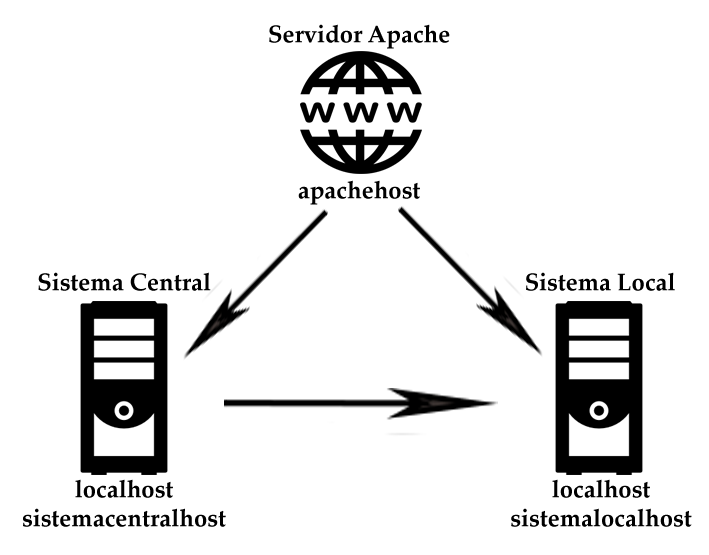
\includegraphics[width=0.7\textwidth]{ligacao_entre_sistemas} % Include the image placeholder.png
		\caption{Representação da ligação entre os sistemas utilizados no projeto e respetivos endereços}
		\label{fig:utilizadores2}
	\end{center}
\end{figure}
\begin{table}
	\centering
	\begin{tabular}{|l|c|c|c|}
		%\hline
		\multicolumn{4}{l}{\textbf{sistema central}} \\ \hline
		\makecell{} & localhost & apachehost & sistemalocalhost \\ \hline
		user & \textbf{X} & \textbf{X} & \\ \hline
		transferencia & \textbf{X} & & \\ \hline
		sensores & & & \\ \hline
		backupmanager & \textbf{X} & & \\ \hline
		\multicolumn{4}{l}{\textbf{sistemas locais}} \\ \hline
		\makecell{} & localhost & apachehost & sistemacentralhost \\ \hline
		user & \textbf{X} & \textbf{X} & \\ \hline
		transferencia & & & \textbf{X} \\ \hline
		sensores & \textbf{X} & & \\ \hline
		backupmanager & & & \\ \hline
	\end{tabular}
	\caption[Tabelas com as limitações dos endereços de conexão das credenciais criadas nos sistemas do projeto]{Tabelas com as limitações dos endereços de conexão das credenciais criadas nos sistemas do projeto. \texttt{localhost}, \texttt{apachehost}, \texttt{sistemalocalhost} e \texttt{sistemacentralhost} representam os endereços do próprio sistema, do servidor \textit{Apache}, dos sistemas locais e do sistema central, respetivamente}
	\label{tab:utilizadores3}
\end{table}

\cleardoublepage
\chapter{Aplicação de Gestão do Sistema}
\label{chap:aplicacao}
A aplicação de gestão do sistema (AGS) foi desenvolvida em ambiente \textit{Web} com o objetivo de ser multiplataforma e permitir acesso remoto e sem recorrer a instalação de \textit{softwares} nos dispositivos dos utilizadores. Corre num servidor \textit{Apache} no sistema central e foi desenvolvida com \textit{PHP}, \textit{JS} e \textit{HTML}. Este capítulo descreve a adaptação da infraestrutura desenvolvida e as várias funcionalidades da AGS.

\section{Adaptação da infraestrutura}
\label{subchap:adap}
A infraestrutura desenvolvida no \autoref{chap:solucao} visa uma utilização a baixo a nível. Ainda que funcional, pode haver margem para erros e incoerência dos dados introduzidos manualmente. A AGS minimiza estas incoerências através da instalação de uma nova BD temporária local no servidor local. Aqui os utilizadores têm a liberdade para adicionar, alterar e apagar informação sem consequências na infraestrutura de dados, antes desta ser introduzida nas BDs central e local como representado na \autoref{fig:adap1}. Como referido anteriormente, esta BD difere das restantes, não contendo em si as tabelas fase e registos.
\begin{figure}[H]
	\begin{center}
		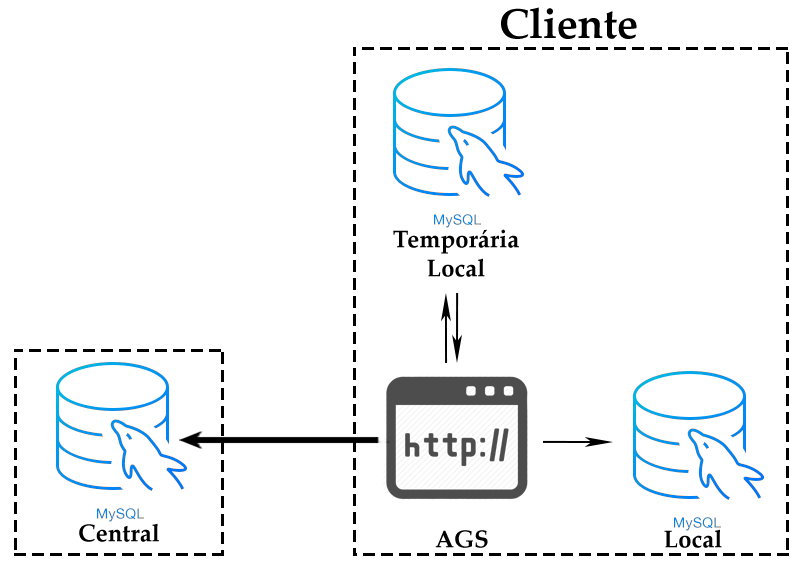
\includegraphics[width=0.56\textwidth]{Aplicacao_temp_local_central} % Include the image placeholder.png
		\caption[Diagrama da ligação AGS-BDs]{Diagrama da ligação AGS-BDs. A AGS comunica com a BD temporária local e depois regista os seus valores nas BDs central e local}
		\label{fig:adap1}
	\end{center}
\end{figure}

\section{Interface gráfica}
A AGS divide-se em quatro partes distintas:
\begin{itemize}[noitemsep]
	\item \textit{Main} - Página principal
	\item \textit{Login} - Página de acesso
	\item Consultas
	\item Administração Local
\end{itemize}
As páginas \textit{Main}, \textit{Login} e Consultas foram realizadas para uma utilização geral. A página Administração Local foi realizada para uma utilização local. A primeira visa um uso a partir de qualquer dispositivo e deve estar acessível a qualquer momento e a segunda foca-se num acesso local com o objetivo de configurar e definir a informação no servidor local. Por outras palavras, para o utilizador usar as funcionalidades desta página tem de aceder à AGS num \textit{browser} no sistema local, que se situa no cliente. As formas como a AGS interage com as bases de dados da infraestrutura desenvolvida numa utilização geral e local, encontram-se nas Figuras \ref{fig:infra_total2} e \ref{fig:infra_total3}, respetivamente.\par 
Instalar um molde é o culminar de um projeto de elevada responsabilidade, esta ideia junto com a criação da BD temporária local serve para melhorar a qualidade da informação introduzida na infraestrutura de dados e diminuir as falhas no processo de instalação deste.\par
As Figuras \ref{fig:aplicacao_simples_consultas} e \ref{fig:aplicacao_simples_admin} representam de forma reduzida os processos de realizar consultas e de configurar e definir a informação nos sistemas locais dos clientes, respetivamente. As versões completas destes fluxogramas podem ser encontradas no \autoref{apen:fluxogramas}.\par
\begin{figure}
	\vspace{0cm}
	\begin{center}
		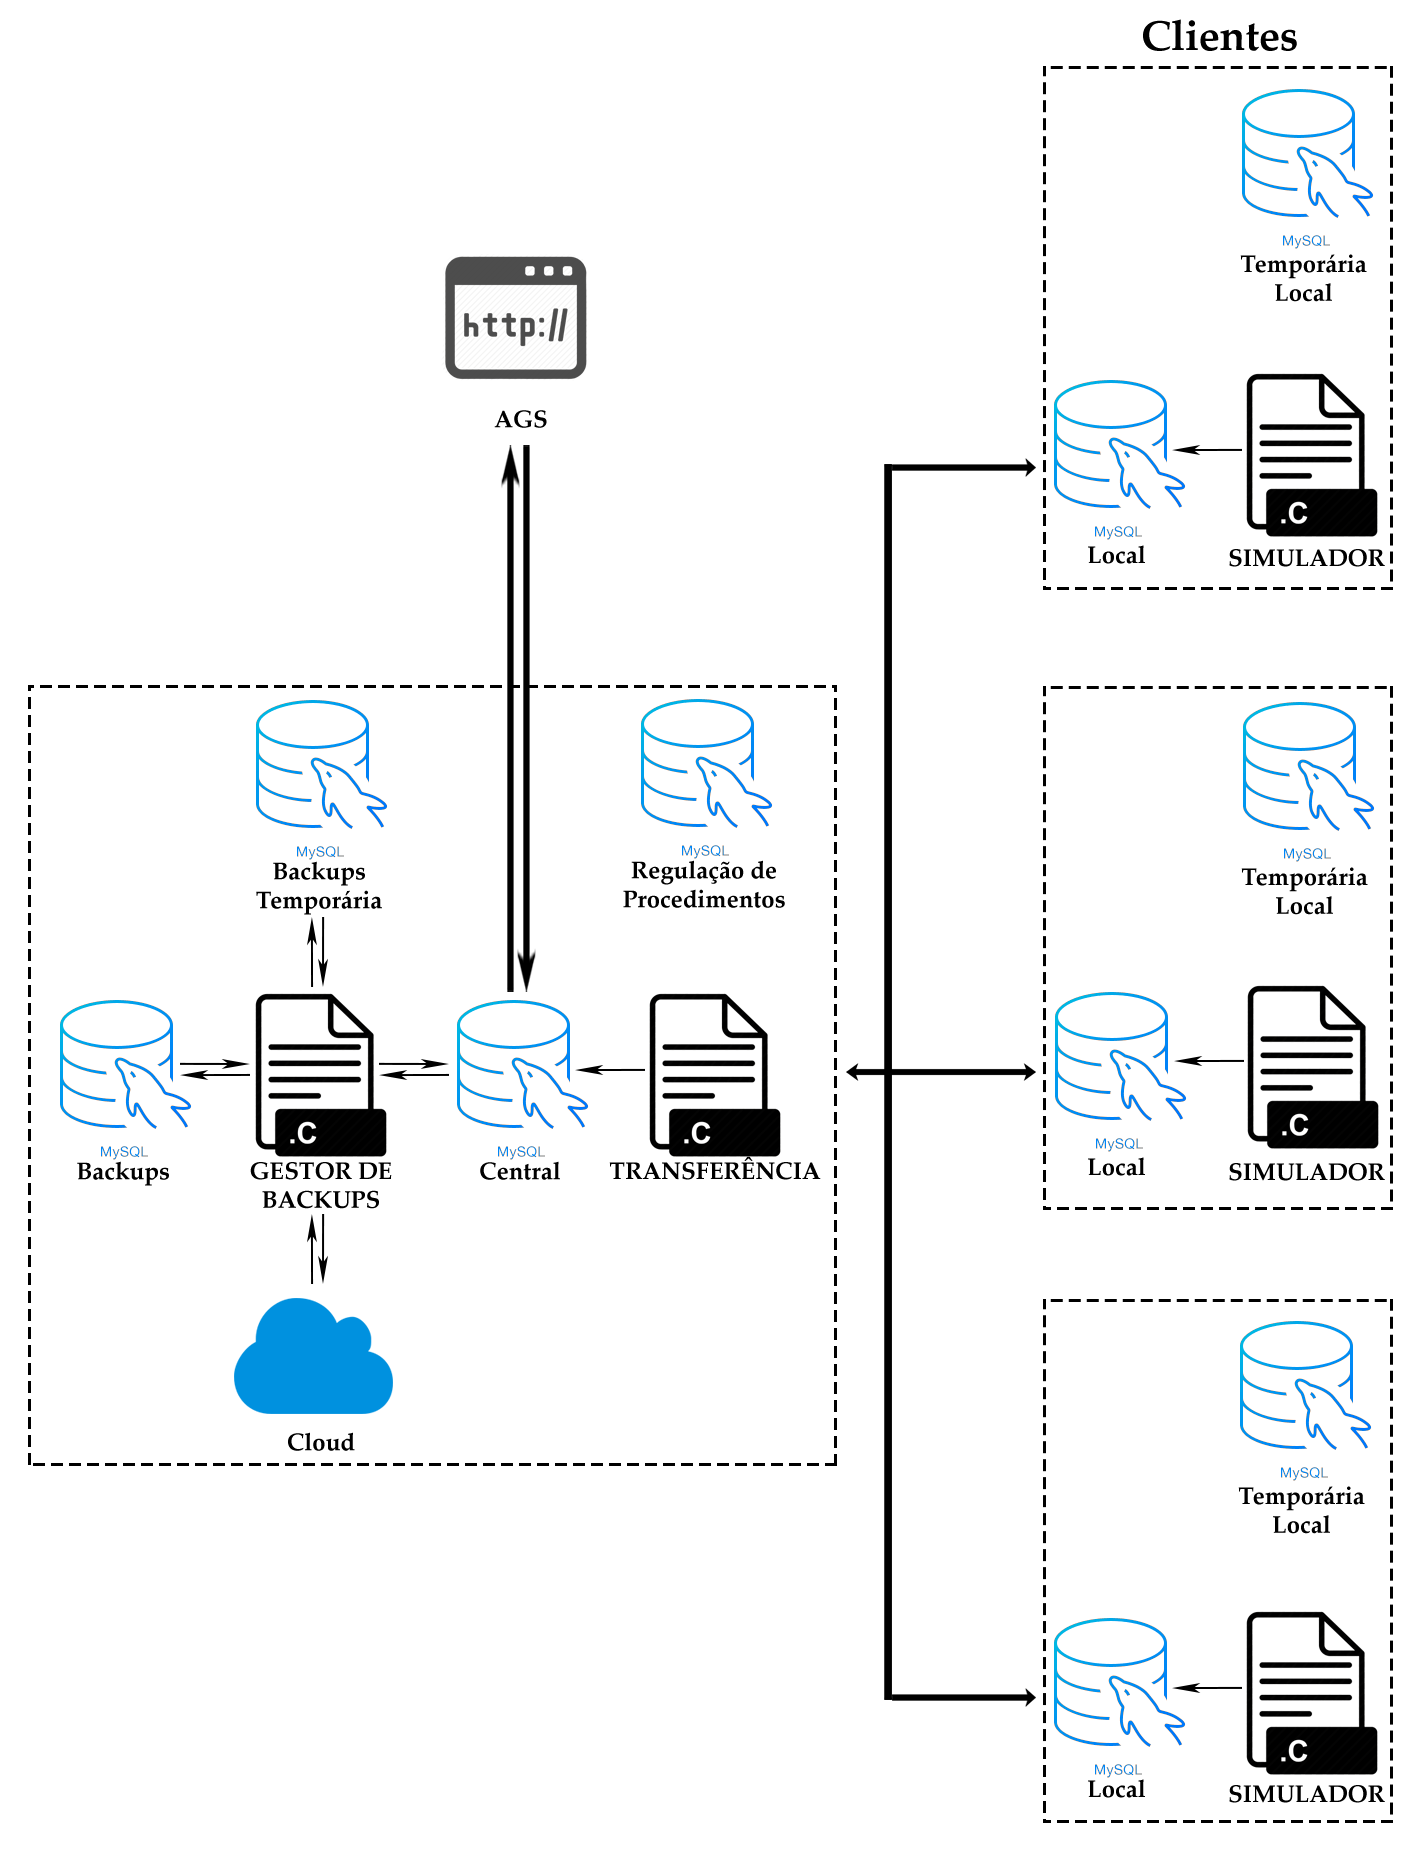
\includegraphics[width=0.95\textwidth]{Esquema_Projeto_Total02} % Include the image placeholder.png
		\caption[Diagrama da infraestrutura completa com uma utilização geral da aplicação de gestão do sistema]{Diagrama da infraestrutura completa com uma utilização geral da AGS. A preto está representado o fluxo de registos. Apesar de não estar representado, os programas de transferência e gestão de \textit{backups} continuam a consultar a BD regulação de procedimentos. Escolheu-se esta representação para salientar que a AGS não interage com estes programas, dado que as funcionalidades Atualizar e Arquivar Molde só estão disponíveis numa utilização local}
		\label{fig:infra_total2}
	\end{center}
\end{figure}
\begin{figure}
	\vspace{0cm}
	\begin{center}
		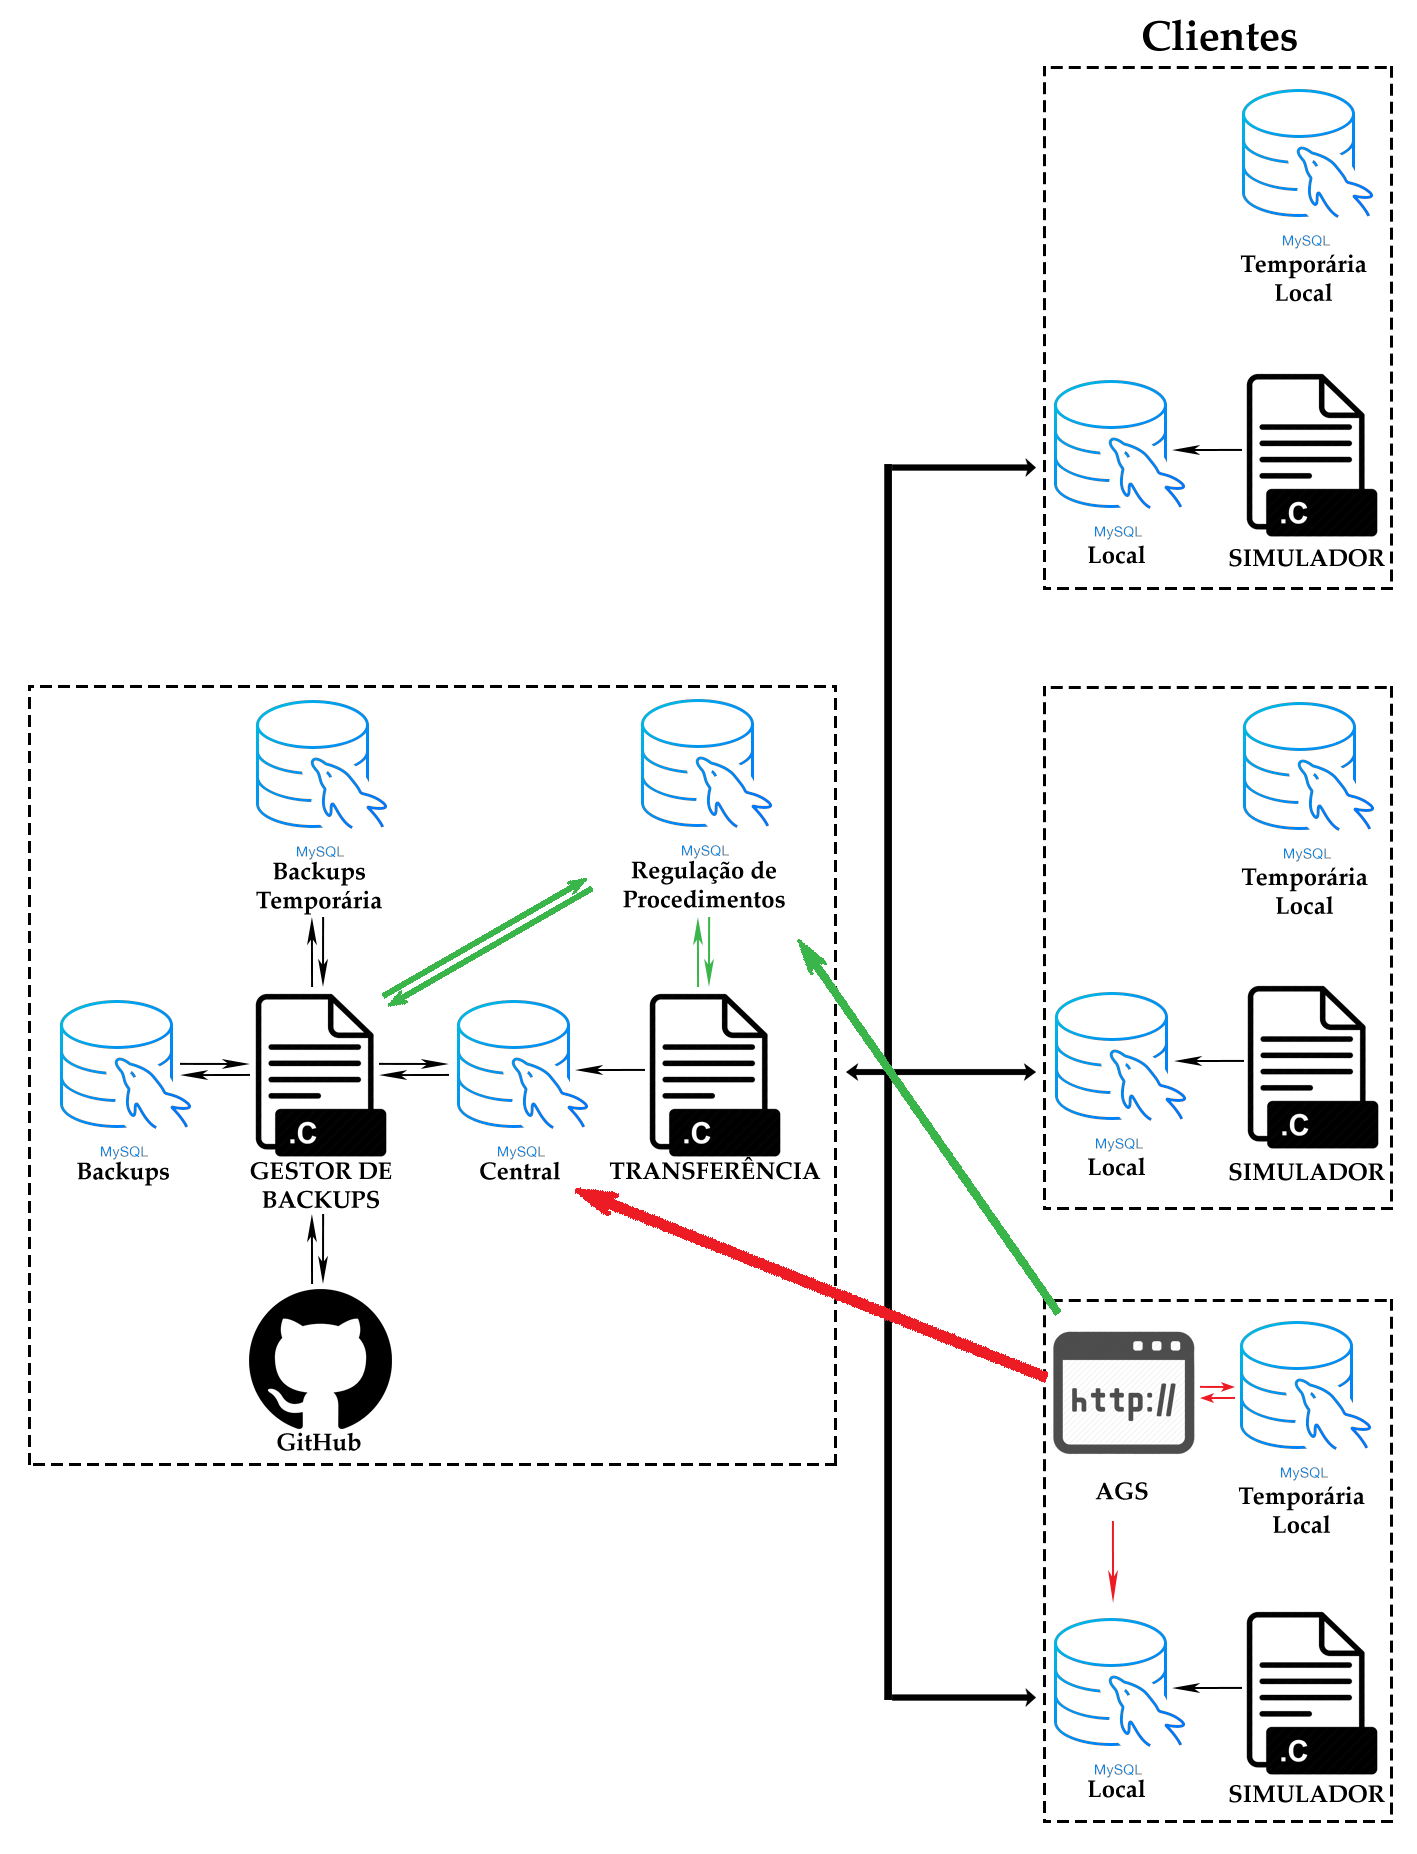
\includegraphics[width=0.95\textwidth]{Esquema_Projeto_Total03} % Include the image placeholder.png
		\caption[Diagrama da infraestrutura completa com uma utilização local da aplicação de gestão do sistema]{Diagrama da infraestrutura completa com uma utilização local da AGS. A preto está representado o fluxo de registos, a verde o fluxo de regulação de procedimentos e a vermelho o fluxo da informação dos clientes, moldes e sensores. Apesar de não estar representado, a AGS continua a poder consultar informação diretamente à BD central como na \autoref{fig:infra_total2}. Escolheu-se não representar para evitar uma saturação da imagem}
		\label{fig:infra_total3}
	\end{center}
\end{figure}
\begin{figure}
	%\vspace{-1.5cm}
	\begin{center}
		\hspace{3.5cm}
		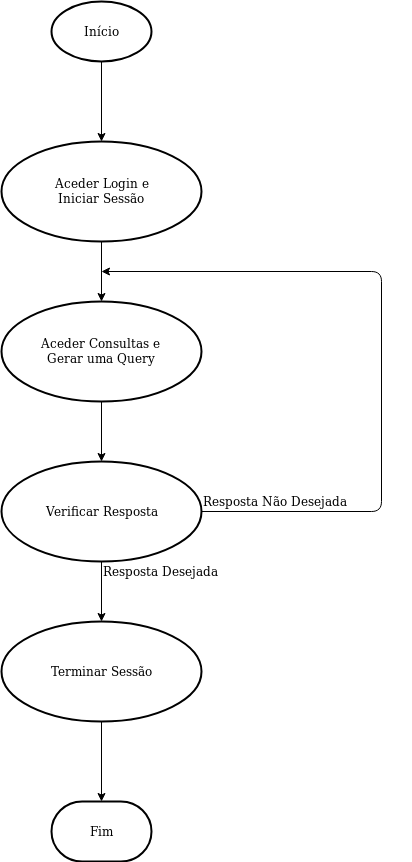
\includegraphics[width=0.5\textwidth]{fluxograma_simples_consultas01} % Include the image placeholder.png
		\caption[Fluxograma reduzido do processo de realizar consultas à base de dados]{Fluxograma reduzido do processo de realizar consultas à base de dados e receber respostas}
		\label{fig:aplicacao_simples_consultas}
	\end{center}
\end{figure}
\begin{figure}
	%\vspace{-2.5cm}
	\begin{center}
		\hspace{3.5cm}
		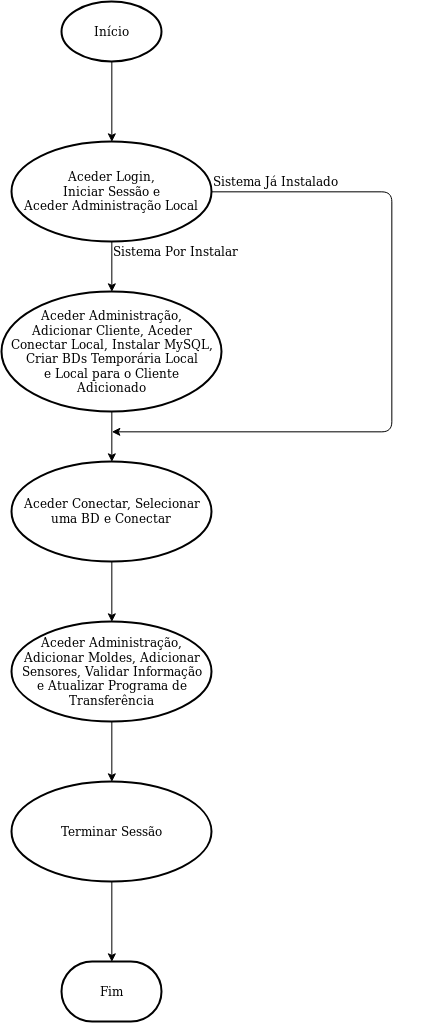
\includegraphics[width=0.5\textwidth]{fluxograma_simples_administracao01} % Include the image placeholder.png
		\caption[Fluxograma reduzido do processo de configurar e definir informação no sistema local do cliente]{Fluxograma reduzido do processo de configurar e definir informação no sistema local do cliente}
		\label{fig:aplicacao_simples_admin}
	\end{center}
\end{figure}

\newpage
\subsection{\textit{Main}}
\begin{figure}[H]
\centering
	\begin{minipage}{1.\textwidth}
		\begin{center}
			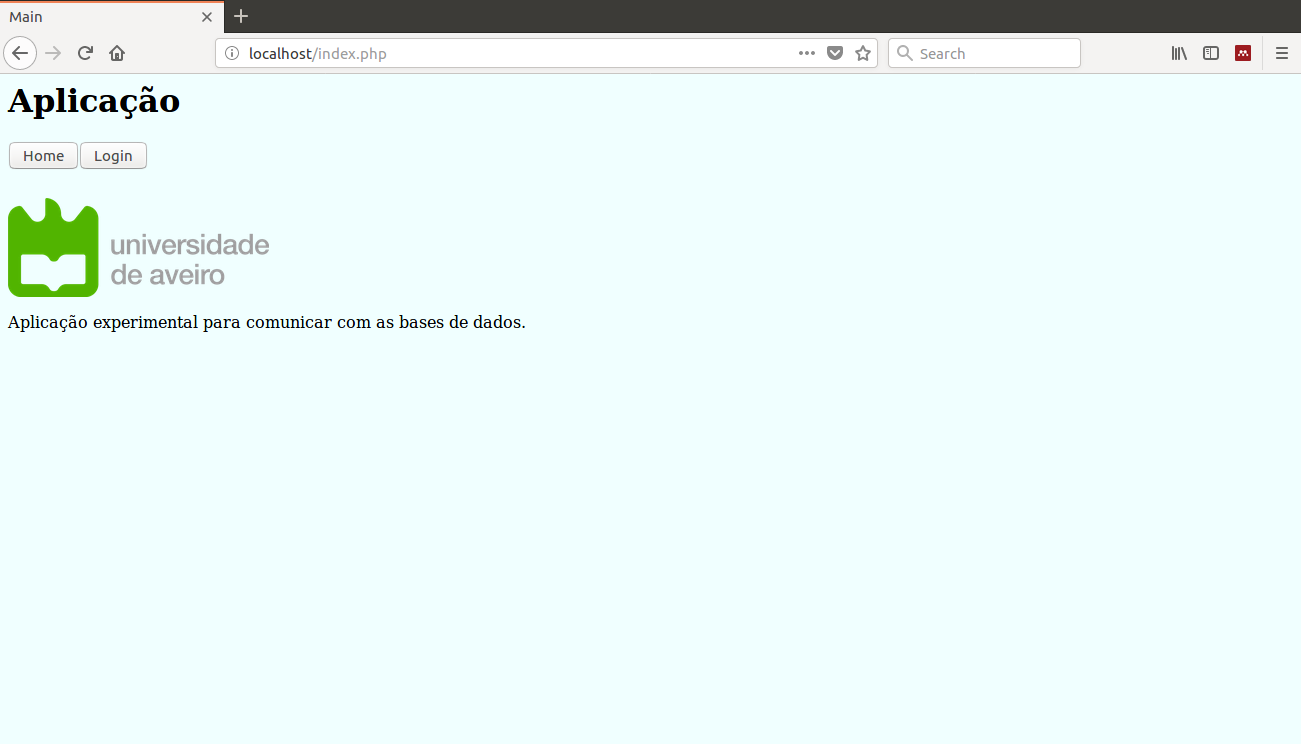
\includegraphics[trim={0 11cm 0 0},clip,width=1\textwidth]{main01} % Include the image placeholder.png
			\subcaption{Sem \textit{login}}
			\label{fig:main1}
		\end{center}
	\end{minipage}
	\begin{minipage}{1.\textwidth}
		\begin{center}
			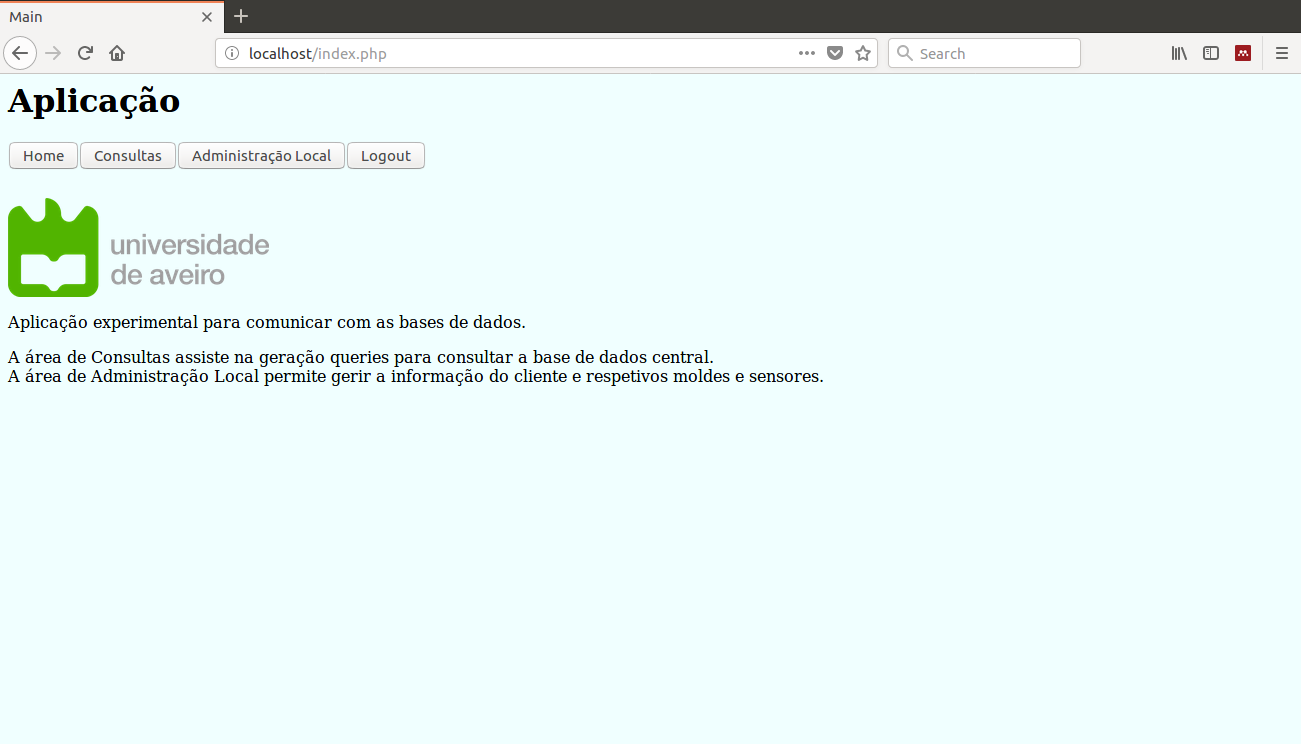
\includegraphics[trim={0 11cm 0 0},clip,width=1\textwidth]{main02} % Include the image placeholder.png
			\subcaption{Com \textit{login}}
			\label{fig:main2}
		\end{center}
	\end{minipage}
	\caption{Funcionalidades da página \textit{Main} com e sem \textit{login}}
	\label{fig:main0}
\end{figure}
\textit{Main} serve como página principal da AGS. Se não houver sessão iniciada, todas as restantes páginas redirecionam o utilizador para aqui. Contém apenas algumas informações gerais sobre a aplicação.\par 
Iniciar sessão na página de \textit{Login} desbloqueia funcionalidades na AGS, como demonstrado nas Figuras \ref{fig:main1} e \ref{fig:main2}. Depois de iniciada a sessão, navega-se com os botões para as páginas de Consultas e Administração Local.

\newpage
\subsection{\textit{Login}}
\label{subchap:login}
\begin{figure}[H]
	\begin{center}
		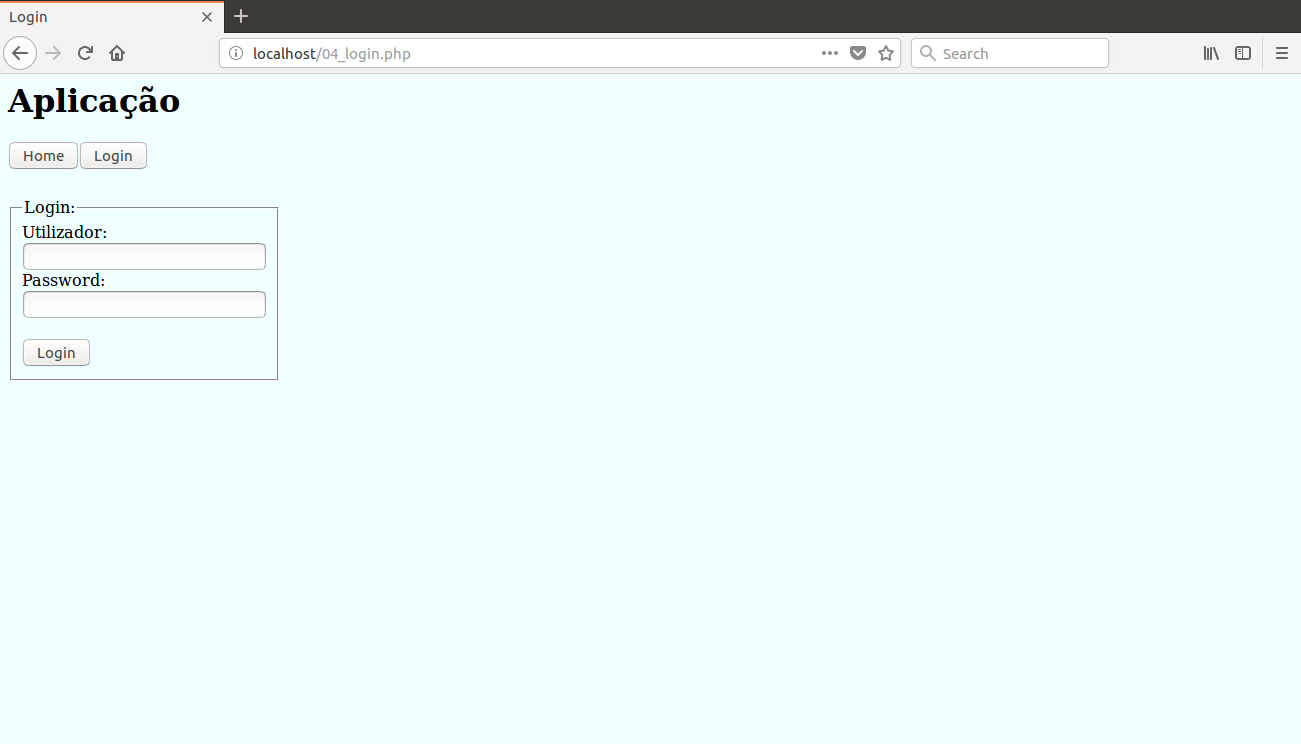
\includegraphics[trim={0 10cm 0 0},clip,width=1\textwidth]{login01} % Include the image placeholder.png
		\caption{Página de \textit{Login} para iniciar sessão na base de dados central}
		\label{fig:login0}
	\end{center}
\end{figure}
A página de \textit{Login} consiste num simples formulário constituído por duas caixas de texto e um botão, como demonstrado na \autoref{fig:login0}. O botão \textit{Login} lê as credenciais introduzidas e realiza uma conexão de teste à BD central validando-as diretamente com \textit{MySQL}. Se as credenciais forem validadas com sucesso redireciona-se o utilizador para a página principal e altera-se o botão de \textit{Login} para \textit{Logout}. Se as credenciais introduzidas não forem suficientes ou válidas são retornados erros de forma a informar o utilizador, como demonstrado nas Figuras \ref{fig:login2} e \ref{fig:login3}.\par 
Quando se acede à página com \textit{Logout} termina-se a sessão e redireciona-se o utilizador para a página principal.
\begin{figure}[H]
	\begin{center}
		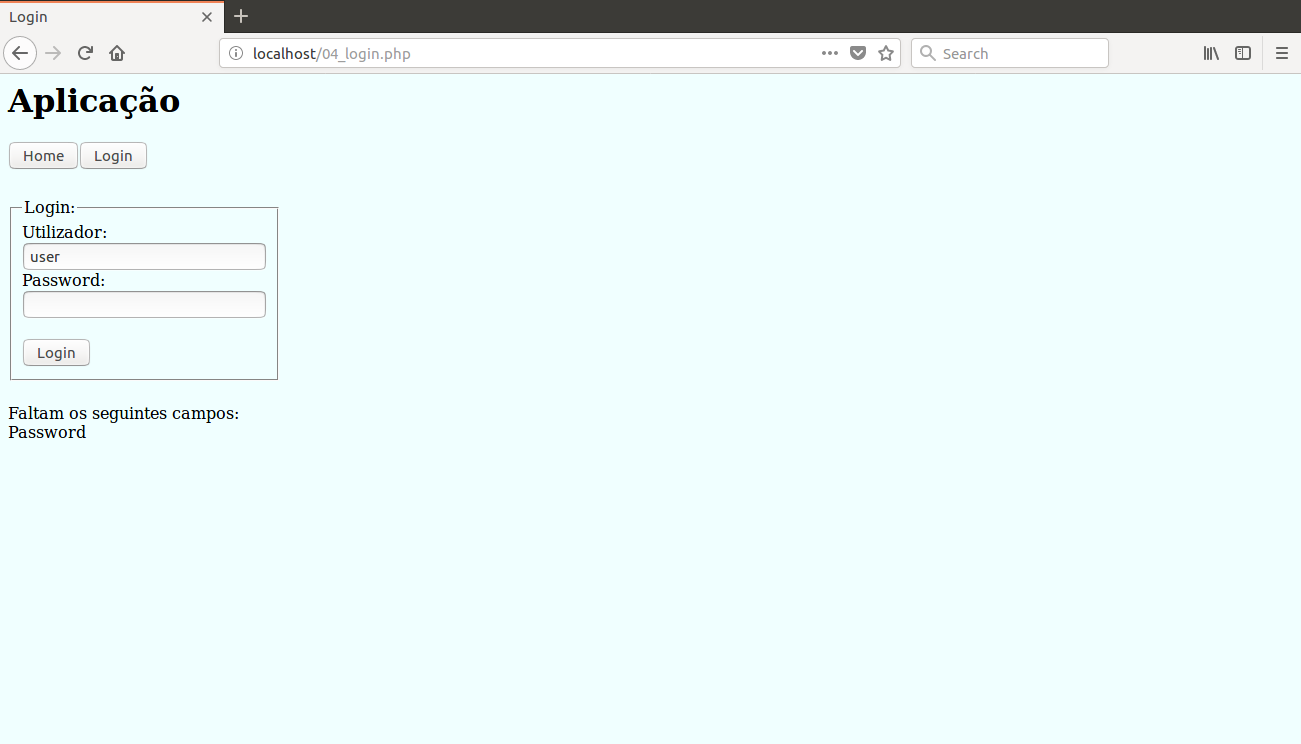
\includegraphics[trim={0 10cm 0 0},clip,width=1\textwidth]{login02} % Include the image placeholder.png
		\caption[Exemplo de erro de falta de informação]{Exemplo de erro de falta de informação retornado quando introduzidas credenciais não válidas na página \textit{Login}}
		\label{fig:login2}
	\end{center}
\end{figure}
\begin{figure}[H]
	\begin{center}
		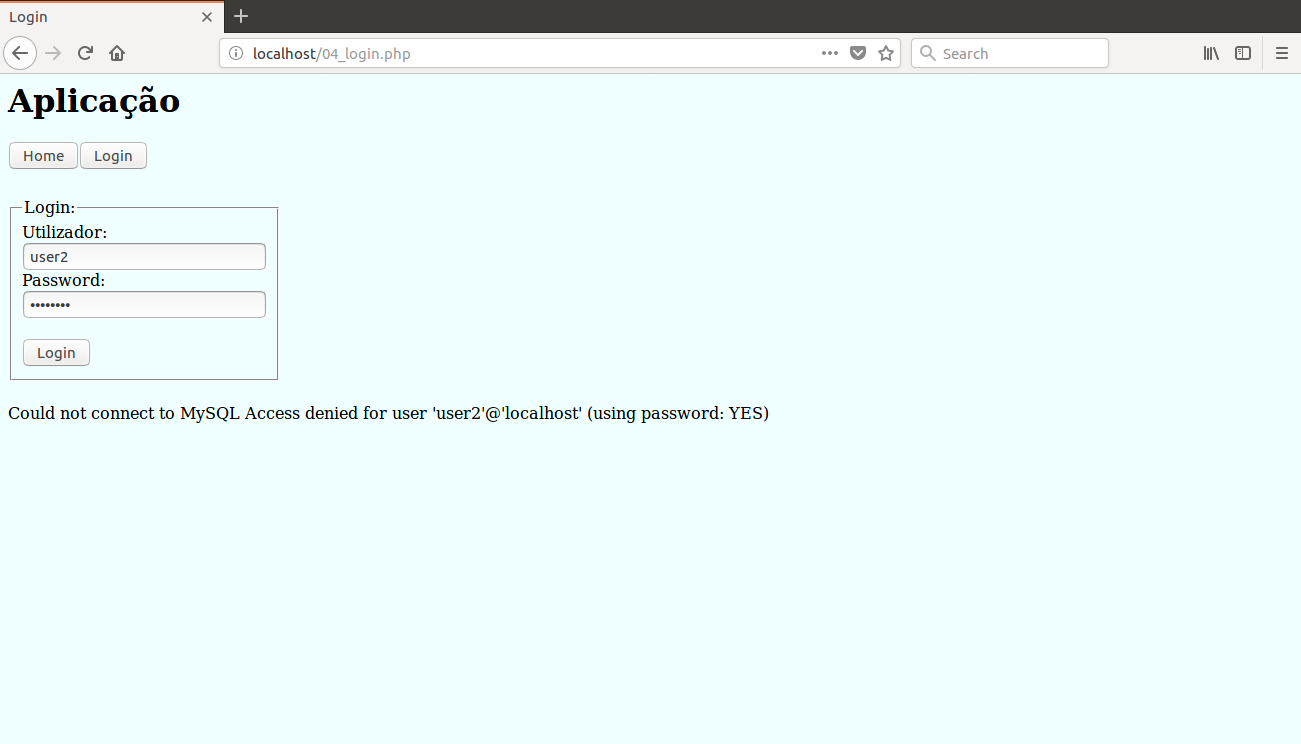
\includegraphics[trim={0 10cm 0 0},clip,width=1\textwidth]{login03} % Include the image placeholder.png
		\caption[Exemplo de erro \textit{MySQL}]{Exemplo de erro \textit{MySQL} retornado quando introduzidas credenciais não válidas na página \textit{Login}}
		\label{fig:login3}
	\end{center}
\end{figure}
%	\caption{Exemplos de erros retornados quando introduzidas credenciais não válidas na página \textit{Login}}
%	\label{fig:login1}

\subsection{Consultas}
\begin{figure}[H]
	\begin{center}
		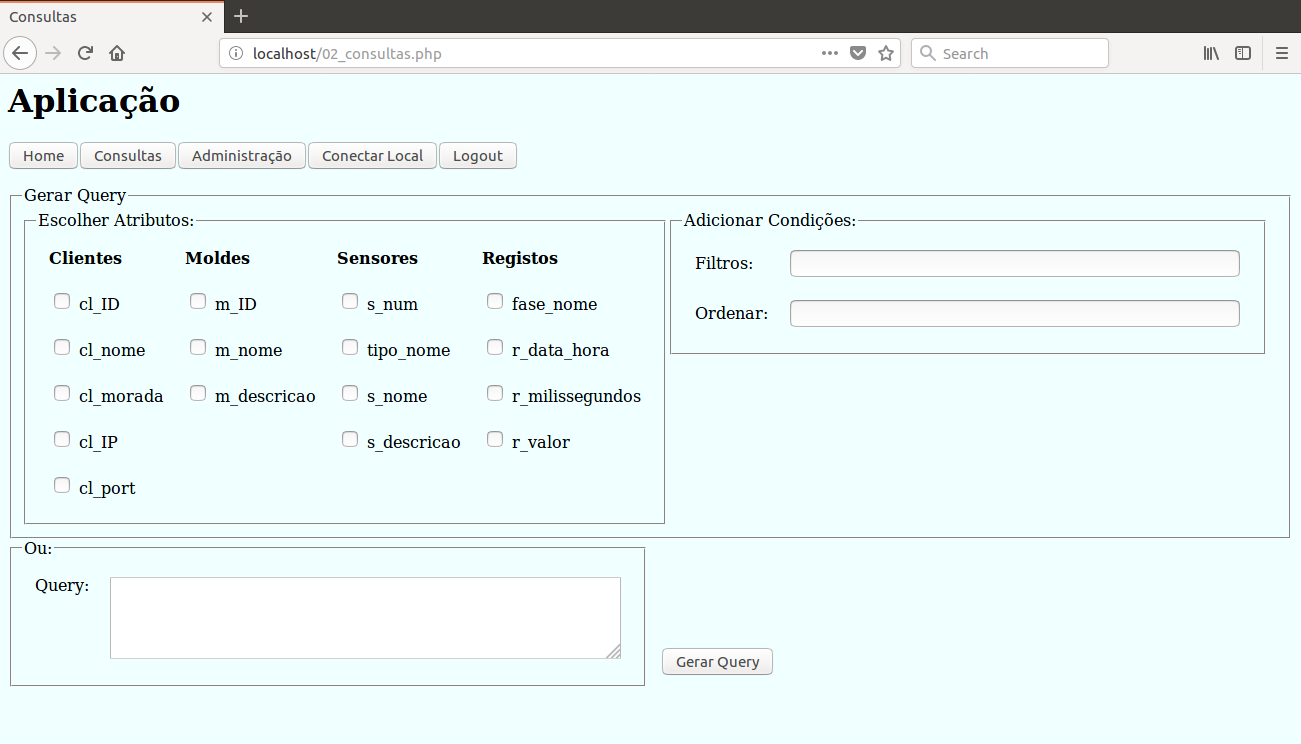
\includegraphics[width=.9\textwidth]{consultas01} % Include the image placeholder.png
		\caption{Página de Consultas que assiste os utilizadores a gerar \textit{queries}}
		\label{fig:consultas1}
	\end{center}
\end{figure}
A página de Consultas assiste os utilizadores sem conhecimentos de \textit{SQL} a gerarem \textit{queries} para consultar a BD central. Na \autoref{fig:consultas1} observa-se várias \textit{checkboxes} e três caixas de texto. As \textit{checkboxes} permitem selecionar os atributos que se desejam consultar na BD; estes atributos são guardados numa variável \texttt{@atributos}.\par 
\newpage
\begin{figure}[H]
	\begin{center}
		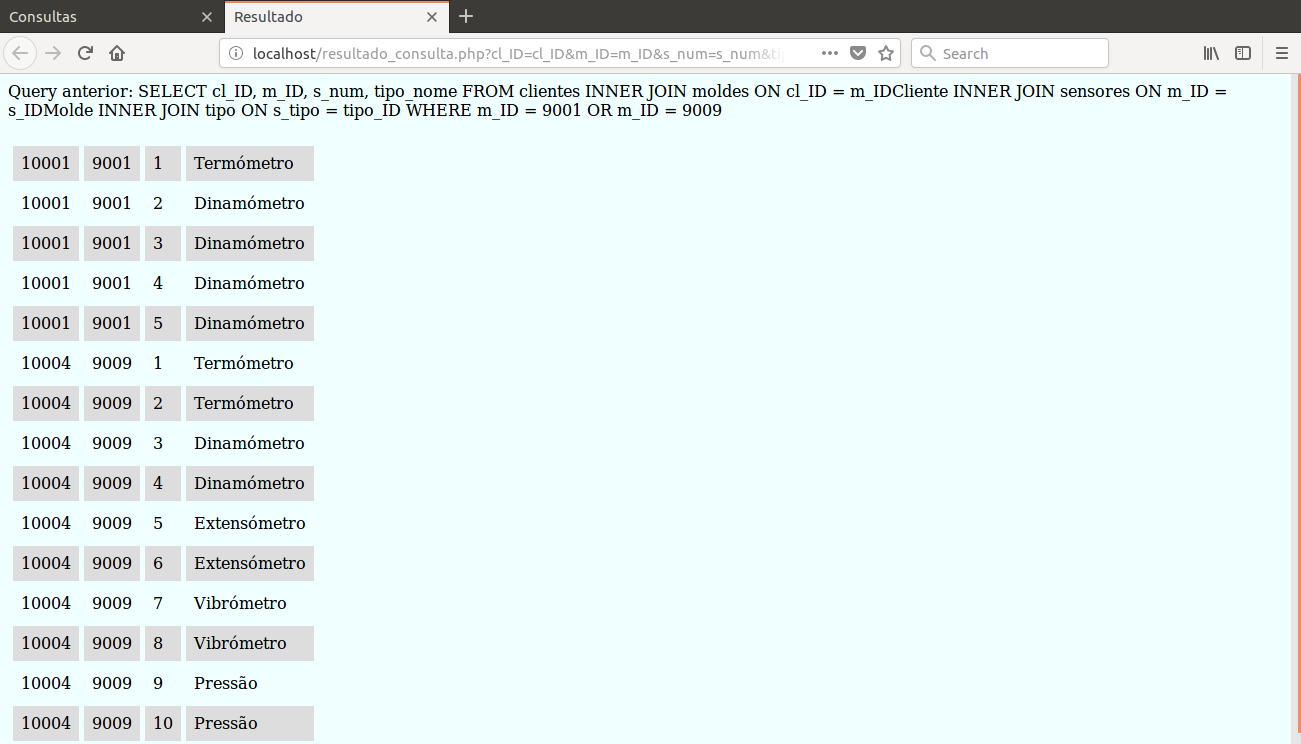
\includegraphics[width=0.9\textwidth]{consultas02} % Include the image placeholder.png
		\caption{Exemplo de resposta a uma consulta}
		\label{fig:consultas2}
	\end{center}
\end{figure}
%	\caption{Página de Consultas e exemplo de resposta a uma consulta}
%	\label{fig:consultas0}
Quando  se prime o botão Gerar Query gera-se uma das seguintes quatro \textit{queries}:
\begin{lstlisting}[language = SQL]
1-	SELECT @atributos
	FROM clientes;
	
2-	SELECT @atributos
	FROM clientes
	INNER JOIN moldes ON cl_ID = m_IDCliente;
	
3-	SELECT @atributos
	FROM clientes
	INNER JOIN moldes ON cl_ID = m_IDCliente
	INNER JOIN sensores ON m_ID = s_IDMolde
	INNER JOIN tipo ON s_tipo = tipo_ID;
	
4-	SELECT @atributos FROM clientes
	INNER JOIN moldes ON cl_ID = m_IDCliente
	INNER JOIN sensores ON m_ID = s_IDMolde 
	INNER JOIN tipo ON s_tipo = tipo_ID
	INNER JOIN registos ON s_IDMolde = r_IDMolde
	AND s_num = r_numSensor
	INNER JOIN fase ON r_fase = fase_ID;
\end{lstlisting}
A seleção é feita com base na coluna mais à esquerda a que os atributos pertencem. Explicando melhor com um exemplo: se o utilizador desejar consultar o \texttt{cl\char`_ID} e o \texttt{cl\char`_nome} da coluna clientes gera-se a primeira \textit{query} no entanto, se o utilizador desejar consultar os atributos \texttt{cl\char`_ID}, \texttt{m\char`_ID} e \texttt{s\char`_num} gera-se a terceira \textit{query}, dado que \texttt{s\char`_num} pertence à terceira coluna.\par
Além destas, foram adicionadas três \textit{queries} especificas quando os atributos \texttt{tipo\char`_}nome, \texttt{fase\char`_nome} e \texttt{r\char`_data}\texttt{\char`_hora} são selecionados sozinhos. As primeiras duas permitem consultar as opções disponíveis nos dicionários e a terceira devolve as datas e horas entre o primeiro e último registos.\par
As caixas de texto Filtros e Ordem na \autoref{fig:consultas1} permitem adicionar às \textit{queries} geradas as cláusulas WHERE e ORDER BY, respetivamente. Assim o utilizador pode obter apenas a informação desejada e ordená-la como quiser. Passando com o cursor por cima destas caixa de texto, visualiza-se um exemplo de como se pode filtrar e ordenar a resposta.\par 
Para os utilizadores com conhecimentos em \textit{SQL} está disponibilizada a caixa de texto \textit{Query} que permite a criação direta de uma \textit{query}. Este campo está limitado apenas para \textit{queries} do tipo SELECT.\par
Depois da \textit{query} ser gerada retorna-se uma resposta num novo separador como demonstrado na \autoref{fig:consultas2}. O \textit{link} desta resposta contém toda a informação da \textit{query} gerada. Este pode ser arquivado ou enviado para outro utilizador sem ser necessário gerar a \textit{query} novamente, isto é útil para \textit{queries} com muitas cláusulas.\par
Se a \textit{query} não for válida retorna-se um erro de forma a informar o utilizador, como demonstrado nas Figuras \ref{fig:consultas4}, \ref{fig:consultas5} e \ref{fig:consultas6}.
\vspace{2cm}
\begin{figure}[H]
	\centering
	\begin{minipage}{1\textwidth}
		\begin{center}
			\includegraphics[trim={0 20cm 0 0},clip,width=1\textwidth]{consultas03} % Include the image placeholder.png
			\subcaption{Erro de informação não introduzida}
			\label{fig:consultas4}
		\end{center}
	\end{minipage}
	\begin{minipage}{1\textwidth}
		\begin{center}
			\includegraphics[trim={0 20cm 0 0},clip,width=1\textwidth]{consultas04} % Include the image placeholder.png
			\subcaption{Erro de \textit{query} que não é do tipo SELECT}
			\label{fig:consultas5}
		\end{center}
	\end{minipage}
	\begin{minipage}{1\textwidth}
		\begin{center}
			\includegraphics[trim={0 20cm 0 0},clip,width=1\textwidth]{consultas05} % Include the image placeholder.png
			\subcaption{Exemplo de erro \textit{MySQL}}
			\label{fig:consultas6}
		\end{center}
	\end{minipage}
	\caption{Exemplos de erros retornados na página de Resposta da Consulta}
	\label{fig:consultas3}
\end{figure}

\newpage
\subsection{Administração Local}
\begin{figure}[H]
	\centering
	\begin{minipage}{1\textwidth}
		\begin{center}
			\includegraphics[trim={0 13cm 0 0},clip,width=1\textwidth]{administracao01} % Include the image placeholder.png
			\subcaption{Sem conexão local}
			\label{fig:admin1}
		\end{center}
	\end{minipage}
	\begin{minipage}{1\textwidth}
		\begin{center}
			\includegraphics[trim={0 13cm 0 0},clip,width=1\textwidth]{administracao02} % Include the image placeholder.png
			\subcaption{Com conexão local}
			\label{fig:admin2}
		\end{center}
	\end{minipage}
	\caption{Funcionalidades da página Administração Local com e sem conexão local}
	\label{fig:admin0}
\end{figure}
Esta área está dividida em duas componentes distintas. A componente de Administração permite ao utilizador alterar informações sobre os clientes, moldes e sensores. A componente de Conectar Local permite realizar uma conexão ao sistema local do cliente. Algumas funcionalidades da componente de Administração só podem ser acedidas quando for efetuada uma conexão à BD local. Após a conexão ser bem sucedida observa-se informação do cliente, como demonstrado nas Figuras \ref{fig:admin1} e \ref{fig:admin2}:
\begin{lstlisting}[language = SQL]
	SELECT cl_ID, cl_nome, COUNT(DISTINCT m_ID),
	COUNT(DISTINCT s_IDMolde, s_num)
	FROM clientes LEFT OUTER JOIN moldes ON cl_ID = m_IDCliente
	LEFT OUTER JOIN sensores ON m_ID = s_IDMolde
	GROUP BY cl_ID;
\end{lstlisting}

\subsubsection{Administração}
Esta componente está dividida em três áreas: Gestão de Clientes, Gestão de Moldes e Gestão de Sensores. No entanto, as áreas de Gestão de Moldes e Gestão de Sensores e as opções de Alterar Cliente, Atualizar, Ver Moldes e Ver Sensores só podem ser utilizadas quando for realizada uma conexão local, como demonstrado na \autoref{fig:admin3}.\par
\begin{figure}[H]
	\begin{center}
		\includegraphics[width=1\textwidth]{administracao03} % Include the image placeholder.png
		\caption{Área de Gestão de Clientes sem conexão local}
		\label{fig:admin3}
	\end{center}
\end{figure}
Quando se acede a esta componente, redireciona-se o utilizador diretamente para a área de Gestão de Clientes. Sem a conexão local realizada, o utilizador só pode adicionar clientes. O botão Adicionar Cliente executa uma \textit{query} do tipo INSERT com a informação introduzida no formulário. Se as informações introduzidas não forem suficientes ou válidas são retornados erros de forma a informar o utilizador, como na \autoref{subchap:login}. Pela AGS não se pode eliminar um cliente depois deste ter sido adicionado à infraestrutura de dados.\par
Após ser estabelecida uma conexão local, a opção de Adicionar Cliente não pode ser utilizada mas, podem-se utilizar as funcionalidades que estavam bloqueadas, como demonstrado na \autoref{fig:admin4}.\par 
O botão Alterar Cliente executa uma \textit{query} do tipo UPDATE, dando ao utilizador a capacidade de alterar a informação dos clientes. Esta ação está limitada ao cliente presente no sistema local conectado. O botão Atualizar reinicia o programa de transferência de registos. Este realiza uma conexão à BD regulação de procedimentos e altera o parâmetro transferência da tabela atualizar de 0 para 1:
\begin{lstlisting}[language = SQL]
	UPDATE reg_proc.atualizar
	SET a_transferencia = 1
	WHERE a_indice = 1;
\end{lstlisting}

\newpage
\begin{figure}[H]
	\begin{center}
		\includegraphics[trim={0 1.5cm 0 0},clip,width=0.9\textwidth]{administracao04} % Include the image placeholder.png
		\caption{Área de Gestão de Clientes com conexão local}
		\label{fig:admin4}
	\end{center}
\end{figure}
\vspace{-1cm}
As áreas de Gestão de Moldes e Gestão de Sensores demonstradas nas Figuras \ref{fig:admin9} e \ref{fig:admin10}, permitem ao utilizador criar e apagar moldes e sensores, respetivamente. Estes dados são inseridos na BD temporária local, onde o utilizador pode adicionar e eliminar moldes e sensores sem afetar a infraestrutura de dados. Desta forma confirma-se a informação introduzida antes de a inserir permanentemente na infraestrutura. Os botões de Adicionar e Eliminar nestes formulários realizam \textit{queries} do tipo INSERT e DELETE, respetivamente. Se as informações introduzidas não forem suficientes ou válidas são retornados erros de forma a informar o utilizador, como na \autoref{subchap:login}.
\begin{figure}[H]
	\centering
		\includegraphics[width=0.9\textwidth]{administracao05} % Include the image placeholder.png
		\caption{Área de Gestão de Moldes}
		\label{fig:admin9}
\end{figure}
\begin{figure}[H]
	\centering
		\includegraphics[width=0.9\textwidth]{administracao06} % Include the image placeholder.png
		\caption{Área de Gestão de Sensores}
		\label{fig:admin10}
\end{figure}
O botão Arquivar Molde permite ao utilizador iniciar, para o molde selecionado, a componente de concatenar \textit{backups} do programa de gestão de \textit{backups} remotamente:
\begin{lstlisting}[language = SQL]
	INSERT INTO reg_proc.backups VALUES
	(@molde_selecionado);
	UPDATE reg_proc.atualizar
	SET a_backups = 1
	WHERE a_indice = 1;
\end{lstlisting} 
Quando a informação dos moldes e sensores estiver completa, o botão Validar tenta registar os valores presentes na BD temporária local nas BDs central e local. Se a ação não executar com sucesso retorna-se um erro \textit{MySQL} de forma a informar o utilizador. Se a ação executar com sucesso, limpa-se a BD temporária local e os valores são registados permanentemente nas BDs central e local, como representado nas Figuras \ref{fig:admin12} e \ref{fig:admin13}.\par
Depois de inseridos, moldes e sensores não podem ser eliminados via AGS. Esta opção foi removida da AGS para evitar erros, dado que apagar um molde em funcionamento pode fazer com que se percam novos registos.\par 
\begin{figure}
	\centering
	\begin{minipage}{1\textwidth}
		\begin{center}
			\includegraphics[width=0.9\textwidth]{administracao07} % Include the image placeholder.png
			\subcaption{Dados antes de serem validados}
			\label{fig:admin12}
		\end{center}
	\end{minipage}
	\begin{minipage}{1\textwidth}
		\begin{center}
			\includegraphics[width=0.9\textwidth]{administracao08} % Include the image placeholder.png
			\subcaption{Dados após serem validados}
			\label{fig:admin13}
		\end{center}
	\end{minipage}
	\caption[Função do botão Validar]{Função do botão Validar, onde os valores da BD temporária local são transferidos de forma permanente para as BDs central e local}
	\label{fig:admin11}
\end{figure}
Nas várias áreas de gestão existem os botões Ver Clientes, Ver Moldes e Ver Sensores que executam respetivamente as \textit{queries}:
\begin{lstlisting}[language = SQL]
1-	SELECT cl_ID, cl_nome, cl_morada, cl_IP, cl_port,
	COUNT(DISTINCT m_ID), COUNT(DISTINCT s_IDMolde, s_num)
	FROM clientes
	LEFT OUTER JOIN moldes ON cl_ID = m_IDCliente
	LEFT OUTER JOIN sensores ON m_ID = s_IDMolde
	GROUP BY cl_ID
	ORDER BY cl_ID
\end{lstlisting}
\newpage
\begin{lstlisting}[language = SQL]
2-	SELECT m_IDCliente, m_ID, m_nome, m_descricao,
	COUNT(DISTINCT s_IDMolde, s_num)
	FROM clientes
	INNER JOIN moldes ON cl_ID = m_IDCliente
	LEFT OUTER JOIN sensores ON m_ID = s_IDMolde
	GROUP BY m_ID
	ORDER BY m_IDCliente, m_ID
	
3-	SELECT m_IDCliente, s_IDMolde, s_num, tipo_nome,
	s_nome, s_descricao
	FROM moldes
	INNER JOIN sensores ON m_ID = s_IDMolde
	INNER JOIN tipo ON s_tipo = tipo_id
	ORDER BY m_IDCliente, s_IDMolde, s_num
\end{lstlisting}
Estas \textit{queries} fornecem algumas informações contextuais para facilitar a navegação do utilizador. Sem conexão local, o botão Ver Clientes retorna a informação de todos os clientes existentes na BD central. Com conexão local, o botão retorna apenas a informação do cliente a que a AGS está conectada.

\subsubsection{Conectar Local}
\label{subchap:local}
A área de Conectar Local na \autoref{fig:local1} permite realizar uma conexão à BD local no servidor do cliente.
	\begin{figure}[H]
		\centering
			\includegraphics[trim={0 11cm 0 0},clip,width=1\textwidth]{local04} % Include the image placeholder.png
			\caption[Área Conectar Local sem BDs locais]{Área Conectar Local sem BDs locais instaladas no sistema}
			\label{fig:local1}
	\end{figure}
Inicialmente o sistema local do cliente não está preparado para fazer parte da infraestrutura de dados. Assim sendo, a área Instalar \textit{MySQL} na \autoref{fig:local2} descreve os passos para instalar o \textit{MySQL} num sistema \textit{Linux}. O botão Copiar Query contém as \textit{queries} necessárias para a criação da BD temporária local e as respetivas permissões.
\newpage
\begin{figure}[H]
	\centering
	\includegraphics[width=0.8\textwidth]{local01} % Include the image placeholder.png
	\caption{Área Instalar \textit{MySQL} para instalar o \textit{software} com os comandos em \textit{Linux}}
	\label{fig:local2}
\end{figure}
A área Criar Local na \autoref{fig:local3} gera \textit{queries} para criar uma BD para um novo cliente. São considerados novos clientes todos os que não tenham moldes associados a si, esta informação obtém-se com a \textit{query}:
\begin{lstlisting}[language = SQL]
	SELECT cl_ID, cl_nome, cl_morada, cl_IP, cl_port
	FROM
	(SELECT cl_ID, cl_nome, cl_morada, cl_IP, cl_port,
	COUNT(DISTINCT m_ID) AS n_moldes
	FROM clientes
	LEFT OUTER JOIN moldes ON cl_ID = m_IDCliente
	GROUP BY cl_ID) AS contagem
	WHERE n_moldes = 0
\end{lstlisting}
\begin{figure}[H]
	\centering
	\includegraphics[trim={0 11cm 0 0},clip,width=0.8\textwidth]{local02} % Include the image placeholder.png
	\caption[Área Criar Local]{Área Criar Local para selecionar cliente adicionado a fim de se gerar \textit{queries} para criar a BD local}
	\label{fig:local3}
\end{figure}
Escolhendo um cliente válido o botão Criar gera \textit{queries} para efetuar a instalação da BD local e definir as respetivas permissões. Estas \textit{queries} não são visíveis ao utilizador, assim sendo, o botão Copiar Query copia-as para a área de transferência e estas devem ser introduzidas no \textit{MySQL} com o comando colar, como representado na \autoref{fig:local4}.
\begin{figure}[H]
	\begin{center}
		\includegraphics[trim={0 2cm 0 0},clip,width=0.8\textwidth]{local03} % Include the image placeholder.png
		\caption[Área Criar Local com \textit{queries geradas}]{Área Criar Local com \textit{queries} geradas para instalar a BD no sistema local. Contêm também as permissões para os utilizadores, que só podem ser garantidas via \textit{root}, e informação adicional para completar a infraestrutura de dados}
		\label{fig:local4}
	\end{center}
\end{figure}
Voltando a área de Conectar, com recurso à \textit{query}:
\begin{lstlisting}[language = SQL]
	SHOW DATABASES
\end{lstlisting}
Obtém-se todas as BDs instaladas no servidor local, como demonstrado na \autoref{fig:local5}. Do ponto de vista prático, cada cliente só terá uma BD local mas, para efeitos de desenvolvimento do projeto adotou-se esta vertente. O botão Conectar inicia sessão na BD local escolhida e redireciona o utilizador para a página de Administração Local na \autoref{fig:admin2}. O botão Desconectar termina esta sessão e redireciona o utilizador também para a página de Administração Local.
\begin{figure}[H]
	\begin{center}
		\includegraphics[trim={0 3cm 0 0},clip,width=0.8\textwidth]{local05} % Include the image placeholder.png
		\caption[Área Conectar Local com BDs locais]{Área Conectar Local onde se visualiza as BDs instaladas no sistema}
		\label{fig:local5}
	\end{center}
\end{figure}

\cleardoublepage
\chapter{Testes de Usabilidade}
\label{chap:usabilidade}
Para testar as funcionalidades e robustez da AGS, convidaram-se 5 pessoas para realizar testes de usabilidade. Assim, foi possível avaliar o comportamento da AGS, bem como recolher comentários e sugestões para futuros desenvolvimentos.\par 
Foram realizados testes de usabilidade em várias alturas durante o desenvolvimento do projeto. As sugestões recolhidas levaram a AGS até ao seu aspeto atual. Este capítulo descreve a preparação, o plano e os resultados dos testes de usabilidade na versão atual da AGS.

\section{Preparação dos testes}
Na \autoref{fig:usabilidade1} está representada a montagem dos testes de usabilidade, que simula a infraestrutura real com um sistema central e outro local. Como referido no \autoref{chap:aplicacao}, a AGS está dividida em dois tipos de utilização. Focando na utilização geral, esta tem de garantir um acesso a partir de qualquer lugar e dispositivo. Assim sendo, pede-se aos utilizadores que, quando possível, utilizem também os seus dispositivos pessoais nestes testes.
\begin{figure}[H]
	\vspace{0.5cm}
	\begin{center}
		\includegraphics[width=0.9\textwidth]{montagem_testes} % Include the image placeholder.png
		\caption[Diagrama da montagem dos testes de usabilidade]{Diagrama da montagem dos testes de usabilidade. O sistema central está ligado por cabo ao \textit{router} e os restantes dispositivos estão ligados via \textit{Wi-Fi}. Para sistema central usou-se um \textit{Lenovo ideapad 110}, para sistema local um \textit{Lenovo Y50}, para \textit{router} usou-se um \textit{Conceptronic C300BRS4A} e para dispositivo pessoal do utilizador um \textit{smartphone}, \textit{tablet}, portátil ou computador pessoal}
		\label{fig:usabilidade1}
	\end{center}
\end{figure}
Insere-se no sistema central os dados iniciais presentes no \autoref{apen:usabilidade}. Este gera registos para clientes, de forma ao utilizador ter informação para consultar a partir do seu dispositivo. O sistema local, no início do teste, tem apenas um simulador a gerar registos. O objetivo é simular moldes instalados no cliente, que se encontram a gerar registos e o utilizador deve preparar o sistema local de forma a que estes registos comecem a ser transferidos para o sistema central.

\section{Plano dos testes}
Inicialmente, contextualiza-se o utilizador sobre os objetivos e funcionalidades da AGS. Aproveita-se esta fase para recolher algumas informações sobre utilizador:
\begin{itemize}
	\item Ocupação profissional
	\item Grau de acompanhamento do projeto
	\item Grau de conhecimentos sobre \textit{SQL}
\end{itemize}
Esta informação permite traçar um perfil dos utilizadores que participaram nos testes. Passando aos testes propriamente ditos, estes têm duas partes distintas que seguem sensivelmente os processos de realizar consultas e de configurar e definir os sistemas locais dos clientes, como representado nas Figuras \ref{fig:aplicacao_consultas} e \ref{fig:aplicacao_admin}, respetivamente.
Em cada etapa do teste anota-se se o utilizador terminou a tarefa:
\begin{itemize}
	\item Sem problemas - o utilizador não cometeu erros durante a realização da tarefa
	\item Após erro do utilizador - o utilizador cometeu erros durante a realização da tarefa e as mensagens de erro retornadas permitiram ao utilizador adaptar e terminar a tarefa
	\item Após erro da AGS - o utilizador encontrou um erro da AGS durante a tarefa que teve de ser resolvido pelo programador de forma a concluir a tarefa
	\item Não conseguiu terminar - o utilizador encontrou um erro fatal que não o permitiu terminar a tarefa
\end{itemize}
Terminando com uma avaliação por parte do utilizador se a AGS foi capaz de cumprir os objetivos definidos anteriormente.

\subsection{Primeira parte - Consultas}
Como referido no \autoref{chap:aplicacao}, esta parte foi desenvolvida com vista a uma utilização geral. Assim sendo, pediu-se aos utilizadores que usassem, quando possível, um dispositivo pessoal para interagir com a AGS. Anota-se quantos utilizadores utilizaram dispositivos pessoais e qual o dispositivo usaram:
\begin{itemize}
	\item \textit{Smartphone}
	\item \textit{Tablet}
	\item Portátil
\end{itemize}
Depois do utilizador aceder à AGS pelo dispositivo são pedidas as seguintes tarefas:
\begin{enumerate}
	\item Iniciar sessão com as credênciais: user, password
	\item Gerar uma \textit{query} onde se observe: ID e nome dos clientes, ID dos moldes, número e tipo dos sensores e fase, data/hora, milissegundos e valor dos registos
	\item Filtrar a resposta retornada para o cliente com o ID 10005
	\item Copiar o \textit{link} da reposta, terminar a sessão. O utilizador deve reabrir a resposta gerada pelo \textit{link} sem ter de gerar a \textit{query} novamente. Aqui espera-se que o utilizador seja redirecionado para a página principal e que perceba que tem de iniciar sessão e re-introduzir o \textit{link}
\end{enumerate}
Depois do teste ser realizado pede-se aos utilizadores que repitam o processo de forma livre para se obter mais informação sobre a experiência do utilizador. Quando o utilizador tiver terminado recolhem-se comentários e sugestões para implementar em trabalhos futuros.

\subsection{Segunda parte - Sistema Local}
Passando para o dispositivo que simula o sistema local, inicia-se o simulador do cliente 10003 para começar a gerar registos. O utilizador deve preparar o sistema local de forma a que os registos gerados passem a ser armazenados no sistema central. Quando o utilizador aceder à AGS pelo dispositivo local são pedidas as seguintes tarefas:
\begin{enumerate}
	\item Verificar que o cliente com ID 10003 não se encontra no sistema
	\item Adicionar o cliente com ID 10003 e informação aleatória
	\item Instalar e configurar o \textit{MySQL}
	\item Criar base de dados temporária local
	\item Criar base de dados local do cliente adicionado
	\item Conectar à base de dados do cliente adicionado
	\item Alterar o cliente para adicionar o IP e port corretos
	\item Adicionar os moldes 9007 e 9008
	\item Para cada molde adicionar um sensor com o número 1
	\item Validar a informação, registando-a permanentemente no sistema
	\item Atualizar programa de transferência
	\item Verificar que registos estão a ser gerados e transferidos
\end{enumerate}
Mais uma vez, depois do teste ser realizado, pede-se aos utilizadores que repitam o processo de forma livre para se obter mais informação sobre a experiência do utilizador. Quando o utilizador tiver terminado recolhem-se comentários e sugestões para implementar em trabalhos futuros.

\section{Resultados dos testes}
Para testar funcionalidades e robustez da AGS, foram convidadas 5 pessoas para participarem nos testes. Em relação aos utilizadores, 20\% eram estudantes, 40\% eram professores e 40\% tinham outra ocupação, como representado na \autoref{fig:resultados01}. Quanto ao grau de acompanhamento do projeto, 20\% não conheciam o projeto, 40\% conheciam o projeto mas não o seu funcionamento e 40\% conheciam o funcionamento do projeto, como representado na \autoref{fig:resultados02}. Uma auto-avaliação dos utilizadores do grau de conhecimentos sobre \textit{SQL} mostrou que 80\% não tinham conhecimentos, 20\% tinham algum conhecimento e nenhum tinha bons conhecimentos, como demonstrado na \autoref{fig:resultados03}.
\begin{figure}[H]
	\centering
	\hspace{-.25cm}
	\begin{tikzpicture}
	\pie [rotate = 180]{40/Outro,
	40/Professor,20/Estudante}
	\end{tikzpicture}
	\caption{Gráfico da ocupação profissional dos utilizadores}
	\label{fig:resultados01}
\end{figure}
\begin{figure}[H]
	\centering
	\begin{tikzpicture}
	\pie [/tikz/every pin/.style={align=center},
	text=pin,rotate = 180] {40/Conheciam o Projeto, 40/Conheciam o Projeto\\Mas Não o Funcionamento, 20/Não Conheciam o Projeto}
	\end{tikzpicture}
	\caption{Gráfico do grau de acompanhamento do projeto dos utilizadores}
	\label{fig:resultados02}
\end{figure}
\begin{figure}[H]
	\centering
	\hspace{-.75cm}
	\begin{tikzpicture}
	\pie [/tikz/every pin/.style={align=center},
	text=pin,rotate = 180] {0/Tinham\\Conhecimentos, 20/Tinham Alguns\\Conhecimentos, 80/Não Tinham\\Conhecimentos}
	\end{tikzpicture}
	\caption{Gráfico do grau de conhecimentos sobre \textit{SQL} dos utilizadores}
	\label{fig:resultados03}
\end{figure}

\subsection{Resultados da primeira parte}
Na primeira parte, 100\% dos utilizadores usaram um dispositivo pessoal, dos quais 40\% eram \textit{smartphones}, 20\% \textit{tablets} e 40\% portáteis, como demonstrado na \autoref{fig:resultados04}.
\begin{figure}[H]
	\centering
	\hspace{1cm}
	\begin{tikzpicture}
	\pie [rotate = 180] {40/Portáteis, 20/Tablets,40/Smartphones}
	\end{tikzpicture}
	\caption{Gráfico dos dispositivos pessoais utilizados nos testes}
	\label{fig:resultados04}
\end{figure}
\newpage
Passando às etapas desta parte do teste, os resultados são apresentados da \autoref{fig:resultados05} a \autoref{fig:resultados08}:
\begin{enumerate}
	\item Iniciar sessão, 20\% dos utilizadores introduziram credenciais erradas
	\begin{figure}[H]
		\centering
		\begin{tikzpicture}
		\begin{axis}[ 
		xbar, xmin=0, xmax=100,
		xlabel={Percentagem \%},
		symbolic y coords={%
			{Não Conseguiu Terminar},
			{Após Erro da AGS},
			{Após Erro do Utilizador},
			Sem Problemas},
		ytick=data,
		nodes near coords, 
		nodes near coords align={horizontal},
		ytick=data,
		width=10cm,
		height=4.5cm,
		]
		\addplot coordinates {
			(0,{Não Conseguiu Terminar})
			(0,{Após Erro da AGS})
			(20,{Após Erro do Utilizador})
			(80,Sem Problemas)};
		\end{axis}
		\end{tikzpicture}
		\caption{Gráfico do resultado de iniciar sessão}
		\label{fig:resultados05}
	\end{figure}
	\item Gerar uma \textit{query}, 100\% dos utilizadores concluíram a tarefa sem problemas
	\begin{figure}[H]
		\centering
		\begin{tikzpicture}
		\begin{axis}[ 
		xbar, xmin=0, xmax=100,
		xlabel={Percentagem \%},
		symbolic y coords={%
			{Não Conseguiu Terminar},
			{Após Erro da AGS},
			{Após Erro do Utilizador},
			Sem Problemas},
		ytick=data,
		nodes near coords, 
		nodes near coords align={horizontal},
		ytick=data,
		width=10cm,
		height=4.5cm,
		]
		\addplot coordinates {
			(0,{Não Conseguiu Terminar})
			(0,{Após Erro da AGS})
			(0,{Após Erro do Utilizador})
			(100,Sem Problemas)};
		\end{axis}
		\end{tikzpicture}
		\caption{Gráfico do resultado de gerar uma \textit{query}}
		\label{fig:resultados06}
	\end{figure}
	\item Filtrar a resposta retornada, 20\% dos utilizadores tiveram dificuldades em filtrar a \textit{query}. Estes utilizadores tinham em comum o facto de estarem a utilizar os seus \textit{smartphones} que não permitem visualizar o exemplo da caixa de texto Filtrar
\begin{figure}[H]
	\centering
	\begin{tikzpicture}
	\begin{axis}[ 
	xbar, xmin=0, xmax=100,
	xlabel={Percentagem \%},
	symbolic y coords={%
		{Não Conseguiu Terminar},
		{Após Erro da AGS},
		{Após Erro do Utilizador},
		Sem Problemas},
	ytick=data,
	nodes near coords, 
	nodes near coords align={horizontal},
	ytick=data,
	width=10cm,
	height=4.5cm,
	]
	\addplot coordinates {
		(0,{Não Conseguiu Terminar})
		(0,{Após Erro da AGS})
		(20,{Após Erro do Utilizador})
		(80,Sem Problemas)};
	\end{axis}
	\end{tikzpicture}
	\caption{Gráfico do resultado de filtrar a resposta retornada}
	\label{fig:resultados07}
\end{figure}
\newpage
	\item Reabrir a reposta anterior pelo \textit{link} após terminar sessão, 100\% dos utilizadores concluíram a tarefa sem problemas
\begin{figure}[H]
	\centering
	\begin{tikzpicture}
	\begin{axis}[ 
	xbar, xmin=0, xmax=100,
	xlabel={Percentagem \%},
	symbolic y coords={%
		{Não Conseguiu Terminar},
		{Após Erro da AGS},
		{Após Erro do Utilizador},
		Sem Problemas},
	ytick=data,
	nodes near coords, 
	nodes near coords align={horizontal},
	ytick=data,
	width=10cm,
	height=4.5cm,
	]
	\addplot coordinates {
		(0,{Não Conseguiu Terminar})
		(0,{Após Erro da AGS})
		(0,{Após Erro do Utilizador})
		(100,Sem Problemas)};
	\end{axis}
	\end{tikzpicture}
	\caption{Gráfico do resultado de reabrir a reposta anterior pelo \textit{link} após terminar sessão}
	\label{fig:resultados08}
\end{figure}
\end{enumerate}
No final do teste pediu-se aos utilizadores que repetissem o processo de forma livre. Durante toda esta parte do teste, notou-se que nenhum utilizador usou a componente de introduzir uma \textit{query} diretamente. Isto seria de esperar dado que a maioria dos utilizadores não tem conhecimentos de \textit{SQL} e confirma que aplicação cumpre o objetivo de assistir estes utilizadores na geração de \textit{queries}.
Para a componente das Consultas foram recolhidas as seguintes sugestões:
\begin{itemize}
	\item Tornar o exemplo de ajuda nas caixas de texto Filtrar e Ordenar mais visíveis, especialmente para os utilizadores dos \textit{smartphones}
	\item Criar uma \textit{checkbox} para selecionar e anular a seleção dos atributos de uma coluna
	\item Tornar a interface mais simples sem se utilizar cl\texttt{\char`_}, m\texttt{\char`_}, etc.
	\item Quando se utiliza o \textit{link} para reabrir a resposta gerada após terminar sessão, em vez do utilizador ser redirecionado para a página principal, redirecionar o utilizador para página de \textit{Login} e depois abrir diretamente a resposta
	\item Dividir a resposta por páginas
	\item Complementar a resposta com gráficos
\end{itemize}

\newpage
\subsection{Resultados da segunda parte}
Seguindo as etapas desta parte do teste, os resultados são apresentados da \autoref{fig:resultados09} a \autoref{fig:resultados08}:
\begin{enumerate}
	\item Verificar que o cliente não se encontra no sistema, 100\% dos utilizadores concluíram a tarefa sem problemas
	\begin{figure}[H]
		\centering
		\begin{tikzpicture}
		\begin{axis}[ 
		xbar, xmin=0, xmax=100,
		xlabel={Percentagem \%},
		symbolic y coords={%
			{Não Conseguiu Terminar},
			{Após Erro da AGS},
			{Após Erro do Utilizador},
			Sem Problemas},
		ytick=data,
		nodes near coords, 
		nodes near coords align={horizontal},
		ytick=data,
		width=10cm,
		height=4.5cm,
		]
		\addplot coordinates {
			(0,{Não Conseguiu Terminar})
			(0,{Após Erro da AGS})
			(0,{Após Erro do Utilizador})
			(100,Sem Problemas)};
		\end{axis}
		\end{tikzpicture}
		\caption{Gráfico do resultado de verificar que o cliente não se encontra no sistema}
		\label{fig:resultados09}
	\end{figure}
	\item Adicionar o cliente, 100\% dos utilizadores concluíram a tarefa sem problemas
	\begin{figure}[H]
		\centering
		\begin{tikzpicture}
		\begin{axis}[ 
		xbar, xmin=0, xmax=100,
		xlabel={Percentagem \%},
		symbolic y coords={%
			{Não Conseguiu Terminar},
			{Após Erro da AGS},
			{Após Erro do Utilizador},
			Sem Problemas},
		ytick=data,
		nodes near coords, 
		nodes near coords align={horizontal},
		ytick=data,
		width=10cm,
		height=4.5cm,
		]
		\addplot coordinates {
			(0,{Não Conseguiu Terminar})
			(0,{Após Erro da AGS})
			(0,{Após Erro do Utilizador})
			(100,Sem Problemas)};
		\end{axis}
		\end{tikzpicture}
		\caption{Gráfico do resultado de adicionar o cliente}
		\label{fig:resultados10}
	\end{figure}
	\item Instalar e configurar o \textit{MySQL}, 80\% dos utilizadores não conseguiram realizar a tarefa porque, mesmo desinstalando o programa, os seus ficheiros de configuração não eram removidos do sistema
	\begin{figure}[H]
		\centering
		\begin{tikzpicture}
		\begin{axis}[ 
		xbar, xmin=0, xmax=100,
		xlabel={Percentagem \%},
		symbolic y coords={%
			{Não Conseguiu Terminar},
			{Após Erro da AGS},
			{Após Erro do Utilizador},
			Sem Problemas},
		ytick=data,
		nodes near coords, 
		nodes near coords align={horizontal},
		ytick=data,
		width=10cm,
		height=4.5cm,
		]
		\addplot coordinates {
			(80,{Não Conseguiu Terminar})
			(0,{Após Erro da AGS})
			(0,{Após Erro do Utilizador})
			(20,Sem Problemas)};
		\end{axis}
		\end{tikzpicture}
		\caption{Gráfico do resultado de instalar e configurar o \textit{MySQL}}
		\label{fig:resultados11}
	\end{figure}
	\newpage
	\item Criar base de dados temporária, 100\% dos utilizadores concluíram a tarefa sem problemas
	\begin{figure}[H]
		\centering
		\begin{tikzpicture}
		\begin{axis}[ 
		xbar, xmin=0, xmax=100,
		xlabel={Percentagem \%},
		symbolic y coords={%
			{Não Conseguiu Terminar},
			{Após Erro da AGS},
			{Após Erro do Utilizador},
			Sem Problemas},
		ytick=data,
		nodes near coords, 
		nodes near coords align={horizontal},
		ytick=data,
		width=10cm,
		height=4.5cm,
		]
		\addplot coordinates {
			(0,{Não Conseguiu Terminar})
			(0,{Após Erro da AGS})
			(0,{Após Erro do Utilizador})
			(100,Sem Problemas)};
		\end{axis}
		\end{tikzpicture}
		\caption{Gráfico do resultado de criar base de dados temporária}
		\label{fig:resultados12}
	\end{figure}
	\item Criar base de dados local do cliente, 100\% dos utilizadores concluíram a tarefa sem problemas
	\begin{figure}[H]
		\centering
		\begin{tikzpicture}
		\begin{axis}[ 
		xbar, xmin=0, xmax=100,
		xlabel={Percentagem \%},
		symbolic y coords={%
			{Não Conseguiu Terminar},
			{Após Erro da AGS},
			{Após Erro do Utilizador},
			Sem Problemas},
		ytick=data,
		nodes near coords, 
		nodes near coords align={horizontal},
		ytick=data,
		width=10cm,
		height=4.5cm,
		]
		\addplot coordinates {
			(0,{Não Conseguiu Terminar})
			(0,{Após Erro da AGS})
			(0,{Após Erro do Utilizador})
			(100,Sem Problemas)};
		\end{axis}
		\end{tikzpicture}
		\caption{Gráfico do resultado de criar base de dados local do cliente}
		\label{fig:resultados13}
	\end{figure}
	\item Conectar à base de dados local, 100\% dos utilizadores concluíram a tarefa sem problemas
	\begin{figure}[H]
		\centering
		\begin{tikzpicture}
		\begin{axis}[ 
		xbar, xmin=0, xmax=100,
		xlabel={Percentagem \%},
		symbolic y coords={%
			{Não Conseguiu Terminar},
			{Após Erro da AGS},
			{Após Erro do Utilizador},
			Sem Problemas},
		ytick=data,
		nodes near coords, 
		nodes near coords align={horizontal},
		ytick=data,
		width=10cm,
		height=4.5cm,
		]
		\addplot coordinates {
			(0,{Não Conseguiu Terminar})
			(0,{Após Erro da AGS})
			(0,{Após Erro do Utilizador})
			(100,Sem Problemas)};
		\end{axis}
		\end{tikzpicture}
		\caption{Gráfico do resultado de conectar à base de dados local}
		\label{fig:resultados14}
	\end{figure}
	\newpage
	\item Alterar cliente, 20\% dos utilizadores não inseriram toda a informação necessária para alterar um cliente e 20\% dos utilizadores detetaram erros na AGS que tiveram de ser corrigidos a fim de terminar a tarefa
	\begin{figure}[H]
		\centering
		\begin{tikzpicture}
		\begin{axis}[ 
		xbar, xmin=0, xmax=100,
		xlabel={Percentagem \%},
		symbolic y coords={%
			{Não Conseguiu Terminar},
			{Após Erro da AGS},
			{Após Erro do Utilizador},
			Sem Problemas},
		ytick=data,
		nodes near coords, 
		nodes near coords align={horizontal},
		ytick=data,
		width=10cm,
		height=4.5cm,
		]
		\addplot coordinates {
			(0,{Não Conseguiu Terminar})
			(20,{Após Erro da AGS})
			(20,{Após Erro do Utilizador})
			(60,Sem Problemas)};
		\end{axis}
		\end{tikzpicture}
		\caption{Gráfico do resultado de alterar cliente}
		\label{fig:resultados15}
	\end{figure}
	\item Adicionar moldes, 100\% dos utilizadores concluíram a tarefa sem problemas
	\begin{figure}[H]
		\centering
		\begin{tikzpicture}
		\begin{axis}[ 
		xbar, xmin=0, xmax=100,
		xlabel={Percentagem \%},
		symbolic y coords={%
			{Não Conseguiu Terminar},
			{Após Erro da AGS},
			{Após Erro do Utilizador},
			Sem Problemas},
		ytick=data,
		nodes near coords, 
		nodes near coords align={horizontal},
		ytick=data,
		width=10cm,
		height=4.5cm,
		]
		\addplot coordinates {
			(0,{Não Conseguiu Terminar})
			(0,{Após Erro da AGS})
			(0,{Após Erro do Utilizador})
			(100,Sem Problemas)};
		\end{axis}
		\end{tikzpicture}
		\caption{Gráfico do resultado de adicionar moldes}
		\label{fig:resultados16}
	\end{figure}
	\item Adicionar sensores, 100\% dos utilizadores concluíram a tarefa sem problemas
	\begin{figure}[H]
		\centering
		\begin{tikzpicture}
		\begin{axis}[ 
		xbar, xmin=0, xmax=100,
		xlabel={Percentagem \%},
		symbolic y coords={%
			{Não Conseguiu Terminar},
			{Após Erro da AGS},
			{Após Erro do Utilizador},
			Sem Problemas},
		ytick=data,
		nodes near coords, 
		nodes near coords align={horizontal},
		ytick=data,
		width=10cm,
		height=4.5cm,
		]
		\addplot coordinates {
			(0,{Não Conseguiu Terminar})
			(0,{Após Erro da AGS})
			(0,{Após Erro do Utilizador})
			(100,Sem Problemas)};
		\end{axis}
		\end{tikzpicture}
		\caption{Gráfico do resultado de adicionar sensores}
		\label{fig:resultados17}
	\end{figure}
	\newpage
	\item Validar a informação, 40\% dos utilizadores detetaram erros na AGS que tiveram de ser corrigidos a fim de terminar a tarefa. Um dos utilizadores teve um pico de latência do servidor que causou o fecho da aplicação no \textit{browser}, deduziu-se que este pico foi falha do \textit{hardware} utilizado
	\begin{figure}[H]
		\centering
		\begin{tikzpicture}
		\begin{axis}[ 
		xbar, xmin=0, xmax=100,
		xlabel={Percentagem \%},
		symbolic y coords={%
			{Não Conseguiu Terminar},
			{Após Erro da AGS},
			{Após Erro do Utilizador},
			Sem Problemas},
		ytick=data,
		nodes near coords, 
		nodes near coords align={horizontal},
		ytick=data,
		width=10cm,
		height=4.5cm,
		]
		\addplot coordinates {
			(0,{Não Conseguiu Terminar})
			(40,{Após Erro da AGS})
			(0,{Após Erro do Utilizador})
			(60,Sem Problemas)};
		\end{axis}
		\end{tikzpicture}
		\caption{Gráfico do resultado de validar a informação}
		\label{fig:resultados18}
	\end{figure}
	\item Atualizar o programa de transferência, 40\% dos utilizadores não conseguiram terminar a tarefa porque foi detetado um conflito entre programas que não se pode resolver durante o teste e 20\% dos utilizadores encontraram erros na aplicação que tiveram de ser corrigidos a fim de terminar a tarefa
	\begin{figure}[H]
		\centering
		\begin{tikzpicture}
		\begin{axis}[ 
		xbar, xmin=0, xmax=100,
		xlabel={Percentagem \%},
		symbolic y coords={%
			{Não Conseguiu Terminar},
			{Após Erro da AGS},
			{Após Erro do Utilizador},
			Sem Problemas},
		ytick=data,
		nodes near coords, 
		nodes near coords align={horizontal},
		ytick=data,
		width=10cm,
		height=4.5cm,
		]
		\addplot coordinates {
			(40,{Não Conseguiu Terminar})
			(20,{Após Erro da AGS})
			(0,{Após Erro do Utilizador})
			(40,Sem Problemas)};
		\end{axis}
		\end{tikzpicture}
		\caption{Gráfico do resultado de atualizar o programa de transferência}
		\label{fig:resultados19}
	\end{figure}
	\item Verificar registos a serem gerados e transferidos, 40\% dos utilizadores não conseguiram terminar a tarefa por não terem tido sucesso no passo anterior
	\begin{figure}[H]
		\centering
		\begin{tikzpicture}
		\begin{axis}[ 
		xbar, xmin=0, xmax=100,
		xlabel={Percentagem \%},
		symbolic y coords={%
			{Não Conseguiu Terminar},
			{Após Erro da AGS},
			{Após Erro do Utilizador},
			Sem Problemas},
		ytick=data,
		nodes near coords, 
		nodes near coords align={horizontal},
		ytick=data,
		width=10cm,
		height=4.5cm,
		]
		\addplot coordinates {
			(40,{Não Conseguiu Terminar})
			(0,{Após Erro da AGS})
			(0,{Após Erro do Utilizador})
			(60,Sem Problemas)};
		\end{axis}
		\end{tikzpicture}
		\caption{Gráfico do resultado de verificar registos a serem gerados e transferidos}
		\label{fig:resultados20}
	\end{figure}
\end{enumerate}
\newpage
Durante a segunda parte do teste, verificou-se que os utilizadores estavam mais à vontade para gerar \textit{queries} comparativamente à primeira parte. Isto demonstra que a aplicação requer alguma experiência por parte dos utilizadores para puder ser usada eficazmente.\par 
Para a componente da Administração Local foram recolhidas as seguintes sugestões:
\begin{itemize}
	\item Completar automaticamente a informação para alterar o cliente
	\item Adicionar um tutorial na aplicação de como preparar o sistema local
	\item Criar avisos nos botões Validar e Atualizar para que o utilizador não realize estas ações por engano
\end{itemize}
Terminado com a avaliação por parte dos utilizadores, 100\% dos utilizadores concordam que a aplicação cumpre os objetivos de assistir na geração de \textit{queries} e de configurar e definir o sistema local do cliente.

\cleardoublepage
\chapter{Conclusões}
\label{chap:conclusoes}
O desafio proposto consiste em monitorizar sensores remotamente. Para isto definiram-se como objetivos principais desenvolver uma rede de bases de dados relacionais e uma aplicação de gestão do sistema que permitisse interagir com elas. Estes objetivos foram concluídos com sucesso. Este capítulo contém comentários sobre o desempenho da solução desenvolvida e propostas para trabalhos futuros.

\section{Comentários}
\subsection{Infraestrutura de dados}
Em relação à infraestrutura proposta, esta cumpre todos os requisitos propostos de garantir uma transferência segura, confidencial e permanente de valores, criando um histórico dos moldes monitorizados. Consiste numa rede de BDs relacionais com uma central e uma local para cada cliente, o que minimiza a perda de registos em caso de falha de conexão; num programa de transferência de registos que coordena a transferência dos registos para o sistema central que cria históricos das medições dos moldes; noutro de gestão de \textit{backups} que limpa a BD central dos registos mais antigos e arquiva-os em ficheiros num repositório \textit{online}; terminando com simuladores que substituem a aquisição de dados reais e permitem popular as BDs locais.\par 
Neste projeto, para ajudar a distinguir as informações, manteve-se a opção de definir manualmente os IDs dos clientes, moldes e sensores. No entanto, numa solução final, estes IDs devem ser gerados automaticamente de forma incremental para manter as BDs organizadas.\par 
Como definido nos objetivos, esta solução não impõe restrições na instrumentação dos moldes. Para introduzir dados nas BDs locais pode ser utilizado qualquer sistema operativo e linguagem de programação desde que esta tenha protocolos de comunicação com \textit{MySQL} e gere \textit{queries} do tipo:
\begin{lstlisting}[language = SQL]
	INSERT INTO registos
	VALUES
	(molde, sensor, fase, data_hora, milissegundos, valor);
\end{lstlisting}
Na realidade esta infraestrutura pode ser utilizada em qualquer contexto de monitorização remota de sensores desde que seja desenvolvido um modelo de dados apropriado.\par

\subsection{Programa de transferência}
O programa cumpre os objetivos definidos de garantir a conservação e taxa de transferência dos registos gerados, bem como ser simples para permitir a sua portabilidade para outras linguagens de programação.\par
Este foi desenvolvido como sendo centralizado em vez de descentralizado, como demonstrado na \autoref{fig:conclusoes0}. 
Na versão centralizada, o sistema central tem de garantir a transferência de todos os clientes o que pode levar a um maior tempo de utilização do processador e consequente perda de desempenho. A versão descentralizada divide este tempo de utilização do processador pelos clientes dado que têm de ser os sistemas locais a garantir a transferência dos registos. Além disto, nesta versão, o programa de transferência pode ser mais simples dado que não existe necessidade do programa principal se dividir em subprogramas, podendo-se resumir aos passos representados na \autoref{fig:transferencia_subprograma}.
\begin{figure}[H]
	\begin{center}
		\includegraphics[width=0.9\textwidth]{Esquema_Projeto_Descentralizado} % Include the image placeholder.png
		\caption{Diagrama da infraestrutura com múltiplas BDs locais conectadas a uma BD central, com o programa de transferência de registos descentralizado}
		\label{fig:conclusoes0}
	\end{center}
\end{figure}
No entanto, a versão descentralizada tem desvantagens, o aumento do consumo de processador dos sistemas locais, por causa do programa de transferência, pode comprometer o desempenho da aquisição de dados no caso desta necessitar de uma elevada cadência de registos. Outra desvantagem, se for necessário alterar o programa de transferência para adicionar novas funcionalidades, tem de se aceder aos sistemas locais onde estes estão a ser executados. Se o programador encarregue de fazer estas alterações não poder aceder diretamente ao sistema local, porque, por exemplo, o sistema local do cliente está situado num país diferente, tem de se garantir uma conexão remota para se poderem realizar estas alterações. Através desta conexão remota o operador pode modificar o sistema local e as BDs como administrador, o que permite contornar as restrições e seguranças definidas e, consequentemente, comprometer a infraestrutura de dados. Terminando com a questão das permissões das credenciais do programa de transferência na \autoref{tab:utilizadores3}. Na versão centralizada, o sistema central não tem de garantir permissões aos endereços dos sistemas locais, ao contrário da versão descentralizada, que tem de garantir permissões aos endereços de todos os sistemas locais. Esta versão requer um maior controlo dos acessos que complica o processo de criação e definição das credenciais do programa de transferência. Por causa destas desvantagens escolheu-se seguir pela versão centralizada.\par 
O método para reiniciar o programa remotamente pela AGS pode, no entanto, ser melhorado. Atualmente, o programa verifica com base num temporizador a BD regulação de procedimentos. Dependendo deste temporizador pode existir alguma latência entre o ato de alterar o parâmetro \texttt{a\char`_transferencia} e o reiniciar propriamente dito do programa. Seria interessante desenvolver outro método que garanta que este se reinicie sem latência.\par 
A taxa de transferência de registos é definida pela capacidade de processamento do sistema utilizado. Durante o desenvolvimento do projeto testou-se a taxa de transferência do programa com os dados presentes na \autoref{tab:conclusoes0}.
\begin{table}[H]
	\centering
	\begin{tabular}{|l|l|l|l|l|}
		%\hline
		\multicolumn{5}{l}{\textbf{clientes}}\\ \cline{1-5}
		ID & Nome & Nº de Moldes & Nº de Sensores & Registos/Segundo\\ \cline{1-5}
		10001 & Autocolismos \& Company & 4 & 16 & 48 \\ \cline{1-5}
		10002 & Máscaras de Carnaval LDA & 6 & 30 & 90 \\ \cline{1-5}
		10003 & Aperture Science & 2 & 2 & 12 \\ \cline{1-5}
		10004 & Black Mesa & 1 & 10 & 30 \\ \cline{1-5}
		10005 & Vault-Tec Corporation & 1 & 1 & 3 \\ \cline{1-5}
	\end{tabular}
	\caption[Tabela com os dados utilizados para testar a taxa de transferência de registos]{Tabela com os dados utilizados para testar a taxa de transferência de registos, com uma média dos registos gerados por segundo para cada cliente}
	\label{tab:conclusoes0}
\end{table}
A quantidade de registos gerada em cada cliente varia consoante o número de moldes e sensores, por este motivo não faz sentido que seja usada a mesma taxa de transferência para todos os clientes. Assim sendo, sugere-se para futuros desenvolvimentos, criar um método de ajustar automaticamente a taxa de transferência de registos para a quantidade de registos produzidos, diminuindo o tempo de utilização do processador do sistema central.
%Além disto, durante o desenvolvimento do projeto, os simuladores nunca geraram registos com maior taxa do que o que o programa de transferência podia transferir. Se esta taxa for superada, a base de dados local de onde provêm os registos ficará cada vez mais cheia, o que pode levar a problemas de desempenho, e, o programa, não está preparado para responder a situações destas. Sugere-se para futuros desenvolvimentos adaptar o programa de forma a que este possa aumentar automaticamente a sua taxa de transferência de registos. Duas soluções que podem ajudar a atingir este objetivo:
%\begin{itemize}
%	\item Aumentar a capacidade da \textit{string} que guarda os tuplos retornados
%	\item Aumentar a quantidade de subprogramas para cada cliente
%\end{itemize}

\subsection{Gestão de \textit{Backups}}
O programa de gestão de \textit{backups} cumpre os objetivos definidos de gerar \textit{backups}, organizar e limpar a BD central, bem como ser simples para permitir a sua portabilidade para outras linguagens de programação.\par 
Quanto à componente de gerar \textit{backups}, existem algumas limitações no método utilizado. Atualmente, o programa cria os ficheiros de \textit{backup} executando diretamente no terminal o comando \texttt{mysqldump} que permite definir a pasta de destino para o ficheiro criado:
\begin{lstlisting}[language = bash]
	mysqldump -u backupmanager -pbackup1234 backups_temp >
	~/Backups/backup.sql
\end{lstlisting}
Este comando também pode ser usado via \textit{query} para o \textit{MySQL}. No entanto, este não tem permissões para criar ficheiros fora da sua pasta principal. Esta pasta está protegida com permissões de administrador do sistema operativo, o que torna difícil mover os \textit{backups} para o repositório \textit{online}. Na verdade é possível habilitar o \textit{MySQL} para criar ficheiros fora da sua pasta principal, só que isto pode constituir uma falha de segurança dado que se podem enviar comandos para o terminal via \textit{query}.\par 
Como referido na \autoref{subchap:backups} os ficheiros criados via \texttt{mysqldump} funcionam como ponto de restauro e requerem o uso de uma BD intermédia para proceder à sua concatenação. No entanto, foi a solução que permitiu interagir com o repositório \textit{online}.\par 
Uma solução explorada inicialmente para criar \textit{backups} consistia em ficheiros \texttt{.csv} que continham apenas registos com uma \textit{query} do estilo:
\begin{lstlisting}[language = SQL]
	SELECT *
	FROM backups.registos
	WHERE r_IDMolde = @IDMolde
	INTO OUTFILE
	'backup_@IDCliente_@IDMolde_@dataIni_@dataFim.csv'
	FIELDS TERMINATED BY ','
	ENCLOSED BY '"'
	LINES TERMINATED BY '\n'
\end{lstlisting}
Esta solução simplifica o processo de criação e concatenação dos \textit{backups} dado que esta não necessita de uma BD intermédia mas, tem algumas desvantagens. A desvantagem principal, como foi referido anteriormente, é não se poder definir o diretório de criação do ficheiro fora da pasta principal do \textit{MySQL}. Além disto, para os dados poderem ser carregados devidamente, as informações dos clientes, moldes, sensores e registos têm de ser armazenadas separadamente, o que vai gerar uma maior diversidade de ficheiros de \textit{backup}. Isto pode constituir um problema se o planeamento dos ficheiros não for bem efetuado.\par 
Em futuros desenvolvimentos, se for definido que o diretório de criação dos \textit{backups} não é imperativo, deve-se dar ênfase a esta solução dado que o processo de gerar e concatenar \textit{backups} é mais simples e consequentemente mais rápido do que a solução usada neste projeto.\par 
Quanto à componente de concatenar \textit{backups}, esta solução pode não se ter demonstrado útil. Se um molde tiver muitos registos, concatenar os seus \textit{backups} pode ultrapassar a capacidade máxima da base de dados, referida na \autoref{subchap:mysql}. Além disto, se se desejar consultar o histórico de um molde arquivado, pode ser interessante manter os \textit{backups} segmentados. Carregar os \textit{backups} necessários para a consulta é mais rápido do que ter de carregar um \textit{backup} total.\par 
Após uma análise crítica, chegou-se à conclusão que esta solução para arquivar moldes não era útil, ainda assim escolheu-se manter as ideias do processo neste relatório. Concatenar \textit{backups} pode ser útil noutras circunstâncias, como por exemplo, realizar uma consulta que envolvam registos mais antigos que já tenham sido guardados. Dada a relativa complexidade de realizar a concatenação decidiu-se que as ideias desenvolvidas podem servir de base para trabalhos futuros.

\subsection{Aplicação de gestão do sistema}
A AGS cumpre os objetivos propostos de ser multiplataforma e garantir um acesso remoto à BD central, bem como gerir as informações dos clientes, moldes e sensores.\par
As mensagens de erro retornadas diretamente pelo \textit{MySQL}, apesar de conterem bastante informação, não são simples de se perceber. Deve-se melhorar as mensagens de erro retornadas para que o utilizador as perceba mais facilmente.\par 
%Durante o desenvolvimento do projeto e testes de usabilidade verificou-se alguma falta de desempenho por parte da aplicação. Após alguns testes chegou-se à conclusão que esta falta de desempenho se devia ao \textit{hardware} utilizado e que um melhor computador e \textit{router} resolviam este problema.\par 
De momento a AGS está preparada para ter mais que um cliente no sistema local. Quando se transitar para a situação real em que cada sistema só tem um cliente pode-se concatenar o processo de Adicionar Cliente, Instalar \textit{MySQL}, Criar Local e Conectar Local num processo só, como demonstrado nas Figuras \ref{fig:conclusoes1}, \ref{fig:conclusoes11} e \ref{fig:conclusoes12}.
\begin{figure}[H]
	\begin{center}
		\includegraphics[trim={0 10.5cm 0 0},clip,width=1\textwidth]{futuro03} % Include the image placeholder.png
		\caption[Exemplo de quando se clica em Conectar Local pela primeira vez]{Exemplo de quando se clica em Conectar Local pela primeira vez e o sistema local não tem o \textit{MySQL} instalado}
		\label{fig:conclusoes1}
	\end{center}
\end{figure}
\begin{figure}[H]
	\begin{center}
		\includegraphics[trim={0 7cm 0 0},clip,width=1\textwidth]{futuro04} % Include the image placeholder.png
		\caption[Exemplo de quando se clica em Conectar Local pela segunda vez]{Exemplo de quando se clica em Conectar Local pela segunda vez para criar as BDs no sistema local}
		\label{fig:conclusoes11}
	\end{center}
\end{figure}
\begin{figure}[H]
	\begin{center}
		\includegraphics[trim={0 14cm 0 0},clip,width=1\textwidth]{administracao02} % Include the image placeholder.png
		\caption[Exemplo de quando se clica em Conectar Local pela terceira vez]{Exemplo de quando se clica em Conectar Local pela terceira vez em que a conexão é realizada diretamente, sem ser necessário escolher o cliente}
		\label{fig:conclusoes12}
	\end{center}
\end{figure}
A AGS só está preparada para adicionar informação à infraestrutura e instalar o sistema local. Sugere-se para futuros desenvolvimentos, preparar a aplicação para eliminar informação da infraestrutura. Na \autoref{fig:conclusoes5} está um exemplo de um botão Eliminar Cliente que eliminaria a informação relativa do cliente e desinstalaria automaticamente o sistema local.
\begin{figure}[H]
	\begin{center}
		\includegraphics[trim={0 2.5cm 0 0},clip,width=1\textwidth]{futuro01} % Include the image placeholder.png
		\caption[Exemplo da área Gestão de Clientes com a funcionalidade Eliminar Cliente]{Exemplo da área Gestão de Clientes com a funcionalidade Eliminar Cliente, que irá remover toda a informação relativa do cliente e eliminar as BDs locais}
		\label{fig:conclusoes5}
	\end{center}
\end{figure}
Deve ser realizada uma revisão de segurança à AGS. Um programador com intenções maliciosas pode aceder ao sistema pela AGS e realizar comandos que podem comprometer o sistema.\par 
Apesar de serem necessários alguns ajustes de forma a melhorar o desempenho, a solução proposta da infraestrutura de dados e AGS é completamente funcional e pode ser já implementada numa fase experimental.

\newpage
\section{Trabalhos Futuros}
Quanto à infraestrutura dos dados não foi definido como os sensores dos moldes serão ligados ao servidor local. No desenvolvimento deste projeto assumiu-se que todos os moldes estão ligados diretamente ao sistema local. No entanto, isto pode não ser sempre possível de se realizar por motivos físicos. Na \autoref{fig:conclusoes3} está representado um exemplo de um cliente que adquiriu quatro moldes que estão situados em pavilhões diferentes. Os moldes 1 e 2 podem ser facilmente ligados ao sistema local no entanto, dada a distancia aos moldes 3 e 4 pode ser difícil liga-los ao sistema local.\par 
Se se justificar, em vez de se ter um servidor local no cliente, ter um em cada molde. Esta adaptação irá criar uma maior quantidade de BDs locais mas isto não é problemático, se o modelo de dados e o programa de transferência forem adaptados para o efeito.\par
\begin{figure}[H]
	\centering
	\begin{minipage}{0.5\textwidth}
	\begin{center}
		\includegraphics[width=1\textwidth]{exemplo_pavilhoes} % Include the image placeholder.png
		\caption[Exemplo de um cliente com moldes em pavilhões diferentes]{Exemplo de um cliente com\\moldes em pavilhões diferentes, que pode\\dificultar as ligações ao sistema local}
		\label{fig:conclusoes3}
	\end{center}
	\end{minipage}%
	\begin{minipage}{0.5\textwidth}
		\vspace{0.8cm}
		\begin{center}
			\includegraphics[trim={0 9cm 35cm 0},clip,width=0.55\textwidth]{futuro02} % Include the image placeholder.png
			\vspace{0.55cm}
			\caption{Exemplo de área de Registar para criar utilizadores com base no ID de trabalhador e email}
			\label{fig:conclusoes2}
		\end{center}
	\end{minipage}
\end{figure}
Quanto à AGS, sugere-se que após uma apresentação inicial à empresa promotora, seja iniciado um processo iterativo de desenvolvimento para escolher e desenvolver novas funcionalidades que possam ser úteis e que não tenham sido abrangidas neste projeto, como por exemplo, a criação de utilizadores baseado no ID de trabalhador demonstrado na \autoref{fig:conclusoes2}, que pode depois servir para criar históricos das intervenções dos utilizadores nas BDs. Culminando numa estilização da AGS para que esta tenha um aspeto mais amigável ao utilizador.\par 
\newpage
Sugere-se a criação de um sistema de notificações e monitorização automático dos moldes. Durante o desenvolvimento do projeto chegou-se à conclusão de que é impossível para um utilizador analisar manualmente milhões de registos de um molde e concluir se este está a funcionar corretamente. Na \autoref{fig:conclusoes4} está representado um exemplo de um possível comportamento de um molde. Cada ponto representa a média dos registos recolhidos em cada dinamómetro, durante um mês na fase de compactação. Estão representados 10 pontos simbolizando 10 meses de funcionamento de um molde. Observa-se um desvio do centróide do molde ao longo do tempo, até este sair fora da área de funcionamento.\par 
Com uma representação visual parece fácil identificar o comportamento errático do molde no entanto, o utilizador teria de o identificar através de consultas e análise de respostas do estilo da \autoref{fig:consultas1}, todos os meses.
\begin{figure}[H]
	\begin{center}
		\includegraphics[width=0.8\textwidth]{exemplo_molde} % Include the image placeholder.png
		\caption[Exemplo molde com 4 dinamómetros em pontos críticos]{Exemplo molde com 4 dinamómetros em pontos críticos. Cada ponto representa o centróide do molde, de acordo com a média dos valores dos dinamómetros durante um mês na fase de compactação}
		\label{fig:conclusoes4}
	\end{center}
\end{figure}
Para auxiliar os utilizadores a identificar este comportamento, sugere-se criar um programa capaz de correr algoritmos que analisem constantemente o comportamento dos moldes. Este programa pode ser desenvolvido em \textit{softwares} mais sofisticados, como por exemplo \textit{MATLAB}, desde que estes tenham protocolos de comunicação com \textit{MySQL}. Mantendo em mente o ambiente \textit{Web}, sugere-se que este programa notifique os utilizadores via AGS ou via email quando um molde começa a demonstrar um comportamento errático.

%
% The bibliography
%
\cleardoublepage
\bibliographystyle{unsrt}
\bibliography{bib/own/molde.bib,bib/own/base_dados.bib,bib/own/software.bib}

%%\sloppy
%%\printbibliography[prenote=myprenote,title=References]
%\iffalse
%  % Use this is the final version
%  %  unsrt produces numbered entries, sorted by order of citation
%  %  plain produces numbered entries, sorted alphabetically
%  %  other styles are possible (I recommend the harvard package)
%  \bibliographystyle{unsrt}
%  %\bibliographystyle{plain}
%  \bibliography{molde}% replace by the name of name of your .bib file
%\else
%  % An example (the contents of the .bbl file)
%  \begin{thebibliography}{10}
%
%  \bibitem{Eliahou-1-1993-CLBNCL}
%  Shalom Eliahou.
%  \newblock The $3x+1$ problem: New lower bounds on nontrivial cycle lengths.
%  \newblock {\em Discrete Mathematics}, 118(1--3):45--56, 1993.
%
%  \bibitem{Garner-1981-1-OCA}
%  Lynn~E. Garner.
%  \newblock On the collatz $3n+1$ algorithm.
%  \newblock {\em Proceedings of the American Mathematical Society}, 82(1):19--22,
%    May 1981.
%  \end{thebibliography}
%\fi

\cleardoublepage
\appendix
\chapter{\textit{Queries} para instalar a solução desenvolvida}
\label{apen:queries}
A informação contida no \autoref{chap:solucao} permite a realização das \textit{queries} presentes neste apêndice.\par 
\section{Sistema Central}
Para criar as BDs central, \textit{backups} e \textit{backups} temporária:
\begin{lstlisting}[language = SQL]
CREATE TABLE tipo
(
	tipo_ID INT NOT NULL,
	tipo_nome VARCHAR(50) NOT NULL,
	CONSTRAINT REPETIDO_ID_TIPO
		PRIMARY KEY(tipo_ID),
	CONSTRAINT REPETIDO_NOME_TIPO
		UNIQUE(tipo_nome)
);
CREATE TABLE fase
(
	fase_ID INT NOT NULL,
	fase_nome VARCHAR(50) NOT NULL,
	CONSTRAINT REPETIDO_ID_FASE
		PRIMARY KEY(FASE_ID),
	CONSTRAINT REPETIDO_NOME_FASE
		UNIQUE(fase_nome)
);
CREATE TABLE clientes
(
	cl_ID INT NOT NULL,
	cl_nome VARCHAR(50) NOT NULL,
	cl_morada VARCHAR(100),
	cl_IP VARCHAR(50) NOT NULL,
	cl_port INT NOT NULL,
	CONSTRAINT REPETIDO_ID_CLIENTE
		PRIMARY KEY(cl_ID)
);
CREATE TABLE moldes
(
	m_IDCliente INT NOT NULL,
	m_ID INT NOT NULL,
	m_nome VARCHAR(30),
	m_descricao VARCHAR(200),
	CONSTRAINT REPETIDO_ID_MOLDE
		PRIMARY KEY(m_ID),
	CONSTRAINT MOLDE_MAU_ID_CLIENTE
		FOREIGN KEY(m_IDCliente)
		REFERENCES clientes(cl_ID)
			ON DELETE NO ACTION ON UPDATE NO ACTION
);
CREATE TABLE sensores
(
	s_IDMolde INT NOT NULL,
	s_num INT NOT NULL,
	s_tipo INT NOT NULL,
	s_nome varchar(30),
	s_descricao varchar(200),
	CONSTRAINT REPETIDO_NUM_SENSOR
		PRIMARY KEY(s_IDMolde,s_num),
	CONSTRAINT SENSOR_MAU_ID_MOLDE
		FOREIGN KEY(s_IDMolde)
		REFERENCES moldes(m_ID)
			ON DELETE CASCADE ON UPDATE NO ACTION,
	CONSTRAINT SENSOR_MAU_ID_TIPO
		FOREIGN KEY(s_tipo)
		REFERENCES tipo(tipo_ID)
			ON DELETE NO ACTION ON UPDATE NO ACTION
);
CREATE TABLE registos
(
	r_IDMolde INT NOT NULL,
	r_numSensor INT NOT NULL,
	r_fase INT NOT NULL,
	r_data_hora DATETIME NOT NULL,
	r_milissegundos TINYINT NOT NULL,
	r_valor FLOAT,
	CONSTRAINT REPETIDO_REGISTO
		PRIMARY KEY(r_IDMolde, r_numSensor,
			r_data_hora, r_milissegundos),
	CONSTRAINT REGISTOS_MAU_ID_MOLDE_SENSOR
		FOREIGN KEY(r_IDMolde,r_numSensor)
		REFERENCES sensores(s_IDMolde,s_num)
			ON DELETE CASCADE ON UPDATE NO ACTION,
	CONSTRAINT REGISTOS_MAU_ID_FASE
		FOREIGN KEY(r_fase)
		REFERENCES fase(fase_ID)
			ON DELETE NO ACTION ON UPDATE NO ACTION
);
INSERT INTO tipo
VALUES
	(1, "Termometro"),
	(2, "Dinamometro"),
	(3, "Extensometro"),
	(4, "Vibrometro"),
	(5, "Pressao"),
	(6, "Acelerometro X"),
	(7, "Acelerometro Y"),
	(8, "Acelerometro Z");
INSERT INTO fase
VALUES
	(1, "Fecho"),
	(2, "Enchimento"),
	(3, "Compactacao"),
	(4, "Abertura"),
	(5, "Extracao");
\end{lstlisting}
A BD regulação de procedimentos
\begin{lstlisting}[language = SQL]
CREATE TABLE atualizar
(
	a_indice INT NOT NULL,
	a_transferencia INT NOT NULL,
	a_backups INT NOT NULL,
	CONSTRAINT REPETIDO_INDICE_ATUALIZAR
		PRIMARY KEY(a_indice),
	CONSTRAINT ATUALIZAR_MAU_INDICE
		CHECK a_indice = 1,
	CONSTRAINT ATUALIZAR_MAU_TRANSFERENCIA
		CHECK a_transferencia = 0 OR a_transferencia = 1,
	CONSTRAINT ATUALIZAR_MAU_BACKUPS
		CHECK a_backups = 0 OR a_backups = 1
);
CREATE TABLE backups
(
	b_IDMolde INT NOT NULL,
	CONSTRAINT REPETIDO_ID_MOLDE
		PRIMARY KEY(a_indice)
);
INSERT INTO atualizar
VALUES
	(1, 0, 0);
\end{lstlisting}
E definem-se as credenciais com as respetivas permissões. Como o servidor \textit{Apache} está a correr no sistema central, o endereço do servidor é igual ao endereço do sistema central:
\begin{lstlisting}[language = SQL]
CREATE USER 'user'@'localhost'
	IDENTIFIED BY 'password';
GRANT SELECT, INSERT, DELETE, UPDATE
	ON central.tipo TO 'user'@'localhost';
GRANT SELECT, INSERT, DELETE, UPDATE
	ON central.fase TO 'user'@'localhost';
GRANT SELECT, INSERT, DELETE, UPDATE
	ON central.clientes TO 'user'@'localhost';
GRANT SELECT, INSERT, DELETE, UPDATE
	ON central.moldes TO 'user'@'localhost';
GRANT SELECT, INSERT, DELETE, UPDATE
	ON central.sensores TO 'user'@'localhost';
GRANT SELECT, DELETE
	ON central.registos TO 'user'@'localhost';
GRANT SELECT, UPDATE
	ON reg_proc.atualizar TO 'user'@'localhost';
GRANT SELECT, INSERT, DELETE, UPDATE
	ON reg_proc.backups TO 'user'@'localhost';
CREATE USER 'transferencia'@'localhost'
	IDENTIFIED BY 'transferencia1234';
GRANT INSERT
	ON central.registos TO 'transferencia'@'localhost';
GRANT SELECT, UPDATE
	ON reg_proc.atualizar TO 'transferencia'@'localhost';
CREATE USER 'backupmanager'@'localhost'
	IDENTIFIED BY 'backup1234';
GRANT SELECT
	ON central.clientes TO 'backupmanager'@'localhost';
GRANT SELECT
	ON central.moldes TO 'backupmanager'@'localhost';
GRANT SELECT
	ON central.sensores TO 'backupmanager'@'localhost';
GRANT SELECT, DELETE
	ON central.registos TO 'backupmanager'@'localhost';
GRANT SELECT, INSERT, DELETE
	ON backups.* TO 'backupmanager'@'localhost';
GRANT SELECT, INSERT, DELETE
	ON backups_temp.* TO 'backupmanager'@'localhost';
GRANT SELECT, UPDATE
	ON reg_proc.atualizar TO 'backupmanager'@'localhost';
GRANT SELECT, DELETE
	ON reg_proc.backups TO 'backupmanager'@'localhost';
FLUSH PRIVILEGES;
\end{lstlisting}

\section{Sistema Local}
Para criar a BD local utiliza-se as mesmas \textit{queries} para criar a BD central. A BD temporária local assume a forma:
\begin{lstlisting}[language = SQL]
CREATE TABLE tipo
(
	tipo_ID INT NOT NULL,
	tipo_nome VARCHAR(50) NOT NULL,
	CONSTRAINT REPETIDO_ID_TIPO
		PRIMARY KEY(tipo_ID),
	CONSTRAINT REPETIDO_NOME_TIPO
		UNIQUE(tipo_nome)
);
CREATE TABLE clientes
(
	cl_ID INT NOT NULL,
	cl_nome VARCHAR(50) NOT NULL,
	cl_morada VARCHAR(100),
	cl_IP VARCHAR(50) NOT NULL,
	cl_port INT NOT NULL,
	CONSTRAINT REPETIDO_ID_CLIENTE
		PRIMARY KEY(cl_ID)
);
CREATE TABLE moldes
(
	m_IDCliente INT NOT NULL,
	m_ID INT NOT NULL,
	m_nome VARCHAR(30),
	m_descricao VARCHAR(200),
	CONSTRAINT REPETIDO_ID_MOLDE
	PRIMARY KEY(m_ID),
	CONSTRAINT MOLDE_MAU_ID_CLIENTE
		FOREIGN KEY(m_IDCliente) REFERENCES clientes(cl_ID)
			ON DELETE NO ACTION ON UPDATE CASCADE
);
CREATE TABLE sensores
(
	s_IDMolde INT NOT NULL,
	s_num INT NOT NULL,
	s_tipo INT NOT NULL,
	s_nome varchar(30),
	s_descricao varchar(200),
	CONSTRAINT REPETIDO_NUM_SENSOR
		PRIMARY KEY(s_IDMolde,s_num),
	CONSTRAINT SENSOR_MAU_ID_MOLDE
		FOREIGN KEY(s_IDMolde) REFERENCES moldes(m_ID)
			ON DELETE CASCADE ON UPDATE CASCADE,
	CONSTRAINT SENSOR_MAU_ID_TIPO
		FOREIGN KEY(s_tipo) REFERENCES tipo(tipo_ID)
			ON DELETE NO ACTION ON UPDATE CASCADE
);
INSERT INTO tipo
VALUES
	(1, "Termometro"),
	(2, "Dinamometro"),
	(3, "Extensometro"),
	(4, "Vibrometro"),
	(5, "Pressao"),
	(6, "Acelerometro X"),
	(7, "Acelerometro Y"),
	(8, "Acelerometro Z");
\end{lstlisting}
Definem-se as credenciais com as respetivas permissões. Como o servidor \textit{Apache} está a correr no sistema central, o endereço do servidor é igual ao endereço do sistema central:
\begin{lstlisting}[language = SQL]
CREATE USER 'user'@'localhost'
	IDENTIFIED BY 'password';
GRANT SELECT, INSERT, DELETE, UPDATE
	ON local.tipo TO 'user'@'localhost';
GRANT SELECT, INSERT, DELETE, UPDATE
	ON local.fase TO 'user'@'localhost';
GRANT SELECT, INSERT, DELETE, UPDATE
	ON local.clientes TO 'user'@'localhost';
GRANT SELECT, INSERT, DELETE, UPDATE
	ON local.moldes TO 'user'@'localhost';
GRANT SELECT, INSERT, DELETE, UPDATE
	ON local.sensores TO 'user'@'localhost';
GRANT SELECT, INSERT, DELETE, UPDATE
	ON local.tipo TO 'user'@'centralhost';
GRANT SELECT, INSERT, DELETE, UPDATE
	ON local.fase TO 'user'@'centralhost';
GRANT SELECT, INSERT, DELETE, UPDATE
	ON local.clientes TO 'user'@'centralhost';
GRANT SELECT, INSERT, DELETE, UPDATE
	ON local.moldes TO 'user'@'centralhost';
GRANT SELECT, INSERT, DELETE, UPDATE
	ON local.sensores TO 'user'@'centralhost';
GRANT SELECT, INSERT, DELETE, UPDATE
	ON temp_local.* TO 'user'@'centralhost';
CREATE USER 'transferencia'@'centralhost'
	IDENTIFIED BY 'transferencia1234';
GRANT SELECT, DELETE
	ON local.registos TO 'transferencia'@'centralhost';
CREATE USER 'sensores'@'localhost'
	IDENTIFIED BY 'sensores1234';
GRANT INSERT
	ON local.registos TO 'sensores'@'localhost';
FLUSH PRIVILEGES;
\end{lstlisting}

\cleardoublepage
\begin{landscape}
\chapter{Evolução dos Diagramas Entidade/Relação}
\label{apen:DER}
\begin{figure}[H]
	\begin{center}
		\includegraphics[width=1.4\textwidth]{evolucao_der2} % Include the image placeholder.png
		\caption[Primeira iteração do Diagrama Entidade/Relação]{Primeira iteração do DER, esta versão considerava os registos como um atributo multi-valor e composto da entidade sensores. Apesar das tabelas serem as mesmas que a versão presente na \autoref{fig:evolucao_der2}, não se consegue perceber a relação entre sensores e registos}
		\label{fig:evolucao_der1}
	\end{center}
\end{figure}
\begin{figure}
	\begin{center}
		\includegraphics[width=1.4\textwidth]{evolucao_der1} % Include the image placeholder.png
		\caption[Segunda iteração do Diagrama Entidade/Relação]{Segunda iteração do DER, simplificação do DER representado na \autoref{fig:evolucao_der1} onde se traduz o atributo multi-valor composto registos numa entidade, permitindo especificar a chave primária, relação com sensores, cardinalidade e obrigatoriedade}
		\label{fig:evolucao_der2}
	\end{center}
\end{figure}
\begin{figure}
	\begin{center}
		\includegraphics[width=1.4\textwidth]{diagrama_entidade_relacao} % Include the image placeholder.png
		\caption[Terceira iteração do Diagrama Entidade/Relação]{Terceira iteração do DER, com a adição dos dicionários pelos motivos referidos na \autoref{subchap:analise}}
		\label{fig:evolucao_der3}
	\end{center}
\end{figure}
\end{landscape}

\cleardoublepage
\chapter{Fluxogramas completos do funcionamento dos programas}
\label{apen:fluxogramas}
Este apêndice contém os fluxogramas completos dos programas e processos desenvolvidos neste projeto:
\begin{itemize}
	\item As Figuras \ref{fig:transferencia_programa} e \ref{fig:transferencia_subprograma} representam os fluxogramas do programa principal e subprogramas do programa de transferência, respetivamente
	\item As Figuras \ref{fig:backups_programa}, \ref{fig:backups_gerar} e \ref{fig:backups_concatenar} representam os fluxogramas do programa principal, da componente de gerar \textit{backups} e da componente de concatenar \textit{backups} do programa de gestão de \textit{backups}, respetivamente
	\item As Figuras \ref{fig:aplicacao_consultas} e \ref{fig:aplicacao_admin} representam os processos de realizar consultas e de configurar e definir a informação nos sistemas locais dos clientes da AGS, respetivamente
\end{itemize}

\begin{figure}
	\vspace{0cm}
	\begin{center}
		\includegraphics[width=.7\textwidth]{fluxograma_transferencia_programa4} % Include the image placeholder.png
		%\vspace{9cm}
		\caption[Fluxograma do programa principal de transferência]{Fluxograma do programa principal de transferência, que cria subprogramas}
		\label{fig:transferencia_programa}
	\end{center}
\end{figure}
\begin{figure}
	\begin{center}
		\includegraphics[width=0.85\textwidth]{fluxograma_transferencia_subprograma4} % Include the image placeholder.png
		\caption[Fluxograma dos subprogramas de transferência]{Fluxograma dos subprogramas de transferência, que transferirem os registos de cada cliente para a BD central}
		\label{fig:transferencia_subprograma}
	\end{center}
\end{figure}
\begin{figure}
	\begin{center}
		\includegraphics[width=0.7\textwidth]{fluxograma_backups_programa01} % Include the image placeholder.png
		\caption[Fluxograma do programa principal de \textit{backups}]{Fluxograma do programa principal de \textit{backups}, com os temporizadores para gerar ou concatenar \textit{backups}}
		\label{fig:backups_programa}
	\end{center}
\end{figure}
\begin{figure}
	\begin{center}
		\includegraphics[width=1\textwidth]{fluxograma_backups_gerar02} % Include the image placeholder.png
		\caption[Fluxograma da componente de gerar \textit{backups}]{Fluxograma da componente de gerar \textit{backups}. Quando esta chega ao fim retorna ao ciclo do programa principal representado na \autoref{fig:backups_programa}}
		\label{fig:backups_gerar}
	\end{center}
\end{figure}
\begin{figure}
	\begin{center}
		\includegraphics[width=1\textwidth]{fluxograma_backups_concatenar03} % Include the image placeholder.png
		\caption[Fluxograma da componente de concatenar \textit{backups}]{Fluxograma da componente de concatenar \textit{backups}. Quando esta chega ao fim retorna ao ciclo do programa principal representado na \autoref{fig:backups_programa}}
		\label{fig:backups_concatenar}
	\end{center}
\end{figure}
\begin{figure}
	\vspace{-0.25cm}
	\begin{center}
		\includegraphics[width=0.6\textwidth]{fluxograma_consultas01} % Include the image placeholder.png
		\caption[Fluxograma do processo de realizar consultas à base de dados]{Fluxograma do processo de realizar consultas à base de dados e receber respostas}
		\label{fig:aplicacao_consultas}
	\end{center}
\end{figure}
\begin{figure}
	\vspace{-0.25cm}
	\begin{center}
		\includegraphics[width=0.9\textwidth]{fluxograma_administracao03} % Include the image placeholder.png
		\caption[Fluxograma do processo de configurar e definir informação no sistema local do cliente]{Fluxograma do processo de configurar e definir informação no sistema local do cliente}
		\label{fig:aplicacao_admin}
	\end{center}
\end{figure}

\cleardoublepage
\chapter{Dados iniciais dos testes de usabilidade}
%\addcontentsline{toc}{chapter}{Dados iniciais dos testes de usabilidade}
%\renewcommand{\thesubsection}{\Alph{subsection}}
%\subsection{Appendix Subsection}
%\subsection{Another appendix Subsection}
\label{apen:usabilidade}
Este apêndice contém as tabelas que representam os dados iniciais no sistema central para a realização dos testes de usabilidade.
\begin{table}[H]
	\centering
	\begin{tabular}{|l|l|}
		%\hline
		\multicolumn{2}{l}{\textbf{tipo}}\\ \cline{1-2}
		tipo\texttt{\char`_}ID & tipo\texttt{\char`_}nome\\ \cline{1-2}
		1 & Termómetro\\ \cline{1-2}
		2 & Dinamómetro\\ \cline{1-2}
		3 & Extensómetro\\ \cline{1-2}
		4 & Vibrómetro\\ \cline{1-2}
		5 & Pressão\\ \cline{1-2}
		6 & Acelerómetro X\\ \cline{1-2}
		7 & Acelerómetro Y\\ \cline{1-2}
		8 & Acelerómetro Z\\ \cline{1-2}
	\end{tabular}
	\caption[Tabela com os valores iniciais da tabela tipo]{Tabela com os valores iniciais da tabela tipo}
	\label{tab:dados1}
\end{table}
\begin{table}[H]
	\centering
	\begin{tabular}{|l|l|}
		%\hline
		\multicolumn{2}{l}{\textbf{fase}}\\ \cline{1-2}
		fase\texttt{\char`_}ID & fase\texttt{\char`_}nome\\ \cline{1-2}
		1 & Fecho\\ \cline{1-2}
		2 & Enchimento\\ \cline{1-2}
		3 & Compactação\\ \cline{1-2}
		4 & Abertura\\ \cline{1-2}
		5 & Extração\\ \cline{1-2}
	\end{tabular}
	\caption[Tabela com os valores iniciais da tabela fase]{Tabela com os valores iniciais da tabela fase}
	\label{tab:dados2}
\end{table}
\begin{table}
	\centering
	\begin{tabular}{|l|l|l|l|l|}
		%\hline
		\multicolumn{5}{l}{\textbf{clientes}}\\ \cline{1-5}
		cl\texttt{\char`_}ID & cl\texttt{\char`_}nome & cl\texttt{\char`_}morada & cl\texttt{\char`_}IP & cl\texttt{\char`_}port\\ \cline{1-5}
		10001 & Autocolismos \& Company & Rua das sanita, nº 2 & 127.0.0.1 & 3306\\ \cline{1-5}
		10002 & Máscaras de Carnaval LDA & Rua de Elm street, nº 13 & 127.0.0.1 & 3306\\ \cline{1-5}
		%10003 & Aperture Science & Travessa de bolo, nº 404 & 127.0.0.1 & 3306\\ \cline{1-5}
		10004 & Black Mesa & Área 51 & 127.0.0.1 & 3306\\ \cline{1-5}
		10005 & Vault-Tec Corporation & Rua da caixa-forte, nº 1234 & 127.0.0.1 & 3306\\ \cline{1-5}
	\end{tabular}
	\caption[Tabela com os valores iniciais da tabela clientes]{Tabela com os valores iniciais da tabela clientes}
	\label{tab:dados3}
\end{table}
\begin{table}
	\centering
	\begin{tabular}{|l|l|l|l|}
		%\hline
		\multicolumn{4}{l}{\textbf{moldes}}\\ \cline{1-4}
		m\texttt{\char`_}IDCliente & m\texttt{\char`_}ID & 
		m\texttt{\char`_}nome & 
		m\texttt{\char`_}descricao\\ \cline{1-4}
		10001 & 9000 & NULL & NULL\\ \cline{1-4}
		10001 & 9001 & NULL & NULL\\ \cline{1-4}
		10001 & 9002 & NULL & NULL\\ \cline{1-4}
		10001 & 9003 & NULL & NULL\\ \cline{1-4}
		10002 & 9004 & NULL & NULL\\ \cline{1-4}
		10002 & 9005 & NULL & NULL\\ \cline{1-4}
		10002 & 9006 & NULL & NULL\\ \cline{1-4}
		%10003 & 9007 & NULL & NULL\\ \cline{1-4}
		%10003 & 9008 & NULL & NULL\\ \cline{1-4}
		10004 & 9009 & NULL & NULL\\ \cline{1-4}
		10002 & 9010 & NULL & NULL\\ \cline{1-4}
		10002 & 9011 & NULL & NULL\\ \cline{1-4}
		10002 & 9012 & NULL & NULL\\ \cline{1-4}
		10005 & 9013 & NULL & NULL\\ \cline{1-4}
	\end{tabular}
	\caption[Tabela com os valores iniciais da tabela moldes]{Tabela com os valores iniciais da tabela moldes}
	\label{tab:dados4}
\end{table}
\begin{table}
	\centering
	\begin{tabular}{|l|l|l|l|l|}
		%\hline
		\multicolumn{5}{l}{\textbf{sensores}}\\ \cline{1-5}
		s\texttt{\char`_}IDMolde & s\texttt{\char`_}num & s\texttt{\char`_}tipo & s\texttt{\char`_}nome & s\texttt{\char`_}descricao\\ \cline{1-5}
		9000 & 1 & 1 & NULL & NULL\\ \cline{1-5}
		9000 & 2 & 2 & NULL & NULL\\ \cline{1-5}
		9000 & 3 & 2 & NULL & NULL\\ \cline{1-5}
		9000 & 4 & 2 & NULL & NULL\\ \cline{1-5}
		9000 & 5 & 2 & NULL & NULL\\ \cline{1-5}
		9001 & 1 & 1 & NULL & NULL\\ \cline{1-5}
		9001 & 2 & 2 & NULL & NULL\\ \cline{1-5}
		9001 & 3 & 2 & NULL & NULL\\ \cline{1-5}
		9001 & 4 & 2 & NULL & NULL\\ \cline{1-5}
		9001 & 5 & 2 & NULL & NULL\\ \cline{1-5}
		9002 & 1 & 5 & NULL & NULL\\ \cline{1-5}
		9002 & 2 & 3 & NULL & NULL\\ \cline{1-5}
		9002 & 3 & 3 & NULL & NULL\\ \cline{1-5}
		9003 & 1 & 5 & NULL & NULL\\ \cline{1-5}
		9003 & 2 & 3 & NULL & NULL\\ \cline{1-5}
		9003 & 3 & 3 & NULL & NULL\\ \cline{1-5}
		9004 & 1 & 1 & NULL & NULL\\ \cline{1-5}
		9004 & 2 & 2 & NULL & NULL\\ \cline{1-5}
		9004 & 3 & 3 & NULL & NULL\\ \cline{1-5}
		9004 & 4 & 4 & NULL & NULL\\ \cline{1-5}
		9004 & 5 & 5 & NULL & NULL\\ \cline{1-5}
	\end{tabular}
	\caption[Parte 1 de 2 da tabela com os valores iniciais da tabela sensores]{Parte 1 de 2 da tabela com os valores iniciais da tabela sensores}
	\label{tab:dados5}
\end{table}
\begin{table}
	\centering
	\begin{tabular}{|l|l|l|l|l|}
		%\hline
		\multicolumn{5}{l}{\textbf{sensores}}\\ \cline{1-5}
		s\texttt{\char`_}IDMolde & s\texttt{\char`_}num & s\texttt{\char`_}tipo & s\texttt{\char`_}nome & s\texttt{\char`_}descricao\\ \cline{1-5}
		9005 & 1 & 1 & NULL & NULL\\ \cline{1-5}
		9005 & 2 & 2 & NULL & NULL\\ \cline{1-5}
		9005 & 3 & 3 & NULL & NULL\\ \cline{1-5}
		9005 & 4 & 4 & NULL & NULL\\ \cline{1-5}
		9005 & 5 & 5 & NULL & NULL\\ \cline{1-5}
		9006 & 1 & 1 & NULL & NULL\\ \cline{1-5}
		9006 & 2 & 2 & NULL & NULL\\ \cline{1-5}
		9006 & 3 & 3 & NULL & NULL\\ \cline{1-5}
		9006 & 4 & 4 & NULL & NULL\\ \cline{1-5}
		9006 & 5 & 5 & NULL & NULL\\ \cline{1-5}
		%9007 & 1 & 5 & NULL & NULL\\ \cline{1-5}
		%9008 & 1 & 5 & NULL & NULL\\ \cline{1-5}
		9009 & 1 & 1 & NULL & NULL\\ \cline{1-5}
		9009 & 2 & 1 & NULL & NULL\\ \cline{1-5}
		9009 & 3 & 2 & NULL & NULL\\ \cline{1-5}
		9009 & 4 & 2 & NULL & NULL\\ \cline{1-5}
		9009 & 5 & 3 & NULL & NULL\\ \cline{1-5}
		9009 & 6 & 3 & NULL & NULL\\ \cline{1-5}
		9009 & 7 & 4 & NULL & NULL\\ \cline{1-5}
		9009 & 8 & 4 & NULL & NULL\\ \cline{1-5}
		9009 & 9 & 5 & NULL & NULL\\ \cline{1-5}
		9009 & 10 & 5 & NULL & \\ \cline{1-5}
		9010 & 1 & 1 & NULL & NULL\\ \cline{1-5}
		9010 & 2 & 2 & NULL & NULL\\ \cline{1-5}
		9010 & 3 & 3 & NULL & NULL\\ \cline{1-5}
		9010 & 4 & 4 & NULL & NULL\\ \cline{1-5}
		9010 & 5 & 5 & NULL & NULL\\ \cline{1-5}
		9011 & 1 & 1 & NULL & NULL\\ \cline{1-5}
		9011 & 2 & 2 & NULL & NULL\\ \cline{1-5}
		9011 & 3 & 3 & NULL & NULL\\ \cline{1-5}
		9011 & 4 & 4 & NULL & NULL\\ \cline{1-5}
		9011 & 5 & 5 & NULL & NULL\\ \cline{1-5}
		9012 & 1 & 1 & NULL & NULL\\ \cline{1-5}
		9012 & 2 & 2 & NULL & NULL\\ \cline{1-5}
		9012 & 3 & 3 & NULL & NULL\\ \cline{1-5}
		9012 & 4 & 4 & NULL & NULL\\ \cline{1-5}
		9012 & 5 & 5 & NULL & NULL\\ \cline{1-5}
		9013 & 1 & 3 & NULL & NULL\\ \cline{1-5}
	\end{tabular}
	\caption[Parte 2 de 2 da tabela com os valores iniciais da tabela sensores]{Parte 2 de 2 da tabela com os valores iniciais da tabela sensores}
	\label{tab:dados6}
\end{table}

\cleardoublepage

\end{document}
